\documentclass[a4paper,12pt,openright]{book}
\usepackage[a4paper,twoside,inner=2.5cm,outer=2.5cm,bindingoffset=1cm,bottom=3cm]{geometry}

% \usepackage[utf8x]{inputenc}
\usepackage{graphicx}
\usepackage{float}

\usepackage{textcomp}
% \usepackage{amsart}
% \usepackage[english]{babel}
\usepackage[hang,small,bf]{caption}
\usepackage{hyperref}
\usepackage{url}
\usepackage[charter]{mathdesign}
\usepackage{fullpage}                               % Use the full page
% \usepackage{fancyhdr}
% \pagestyle{fancy}
\usepackage{subfig}
\usepackage{pdfpages}

\usepackage{xcolor}
\usepackage{listings}

\usepackage{siunitx}
\usepackage{todonotes}                              % To do notes and figures
% \usepackage[numbers,square,sort&compress]{natbib}   % Bibliography
% Bibliography
\usepackage[
  backend=biber,
  giveninits=true,
  style=numeric-comp
]{biblatex}
\usepackage{nicefrac}                               % Nice fractions
\usepackage[super]{nth}                             % 1st, 2nd, 3rd, ...

% Turbulence block diagrams
\usepackage{tikz}
\usetikzlibrary{shapes,arrows,positioning,calc}

% Nomenclature
% \usepackage{nomencl}
\usepackage{longtable}

% Mathematics
\usepackage{amsmath}
\newcommand{\superscript}[1]{\ensuremath{^{\textrm{#1}}}}
\newcommand{\subscript}[1]{\ensuremath{_{\textrm{#1}}}}
\newcommand{\degree}{\ensuremath{^\circ}}
% \usepackage{nicefrac}
\usepackage{mathtools}
\DeclarePairedDelimiter\ceil{\lceil}{\rceil}
\DeclarePairedDelimiter\floor{\lfloor}{\rfloor}

\setcounter{tocdepth}{2}

% Common things used both in the thesis and in the defence announcement

\newcommand\thesistype{PhD} % PhD or Lic

\newcommand\thesistitle{Auralisation of airplanes considering sound propagation in a turbulent atmosphere}
\newcommand\thesissubtitle{} % if empty leave only {}
\newcommand\thesisauthor{Frederik Rietdijk}

\newcommand{\thesiscoverimage}{../figures/generated/turbulence-parameters/turbulence-1.0-1e-06} % Cover image. Comment away (not leave empty) if not needed
\newcommand{\thesiscoverdescription}{}%Cover: Supervisor for interactive product configuration, see Figure~\ref{fig:kappa-sup} on page~\pageref{fig:kappa-sup}.}  % Leave {} if no description of the cover image needed

\newcommand\thesisdepartment{Architecture and Civil Engineering}
\newcommand\thesiscity{Göteborg}
\newcommand\thesismonth{September} % e.g. January, February...
\newcommand\thesisyear{2017}
\newcommand\thesisisbn{}  % call library to get this number for PhD, leave empty for Lic
\newcommand{\thesisissn}{%
  \ifthenelse{\equal{\thesistype}{PhD}}%
    {ISSN XXXX-XXXX}% For PhD it is Chalmers PhD ISSN (call library to double-check)
    {}% For Lic it is Departmental reports ISSN (ask secretary)
}
\newcommand\thesisnumber{} % for PhD this is "Ny serie nr" and looks like 3452 (call library to get your number), for Lic it is departmental report number and looks like R001 (ask department secretary)

% Defence information
\newcommand\defenceday{XX} % e.g. 14th
\newcommand\defencemonth{\thesismonth} % e.g. January, February...
\newcommand\defenceyear{\thesisyear} % e.g. 2009, 2010...
\newcommand\defencetime{XX:XX} % e.g. 10:00, 13:00...
\newcommand\defenceroom{EA} % e.g. "EA", "HC4"...
\newcommand\defenceaddress{-} % from where the \thesislocation can be accessed
\newcommand\defenceopponent{-}
\newcommand\defenceopponentdepartment{-}
\newcommand\defenceopponentuniversity{-}


\title{\thesistitle}
\author{\thesisauthor}

% \makenomenclature

\bibliography{library.bib}

\begin{document}
\maketitle
\thispagestyle{empty}	% Hide page number.

% Abstract
\newpage\section*{Abstract}Aircraft noise is a major issue in urban areas. Due to a rising level of
urbanisation and the continuing growth of air traffic more people are exposed to
aircraft noise than ever. Methods currently used for assessing the
impact of aircraft noise on humans consider mostly energetic quantities, and not the
dynamic character of the sound. Therefore, in order to obtain a more accurate
picture of the impact of aircraft sound it may be helpful to assess how the audible
sound is perceived.

Auralisation is a method for rendering audible sound fields and may be used to
create audible aircraft sound. A tool was developed to auralise the sound of jet
airplanes and consists of an outdoor sound propagation model and an emission synthesiser.
The emission synthesiser computes an emission signal consisting of tonal
components and broadband noise. The spectral components vary over time and take
into account directivity.

An inverse propagation model was developed to compute back from a receiver to
source in time-domain. An automated procedure was developed to extract features
from the resulting signal. These features were then used to directly synthesise
the emission as function of time, and this signal was propagated to the original
receiver resulting in an auralisation that should reproduce the recording
it is based on.

To validate the auralisation tool, a listening test was conducted where participants
were presented with recordings and auralisations and had to rate their similarity.
Results indicate that differences exist between the auralisations and recordings.
Improving the synthesis of the blade passing frequency is expected to improve the similarity
between auralisations and recordings.

Finally, fluctuations can typically be noticed when listening to sound from a
distant aircraft, and one cause of these fluctuations is atmospheric turbulence.
A computationally fast algorithm was developed to take into account the
amplitude and phase modulations that arise as the sound propagates through the
turbulent atmosphere. According to the author the method results in improved
plausibility of the auralisations.



\vspace{0.1cm}

\textbf{Keywords}: Aircraft noise, Auralisation, Outdoor sound propagation, Atmospheric turbulence

% List of publications
\newpage\input{publications}
% Acknowledgements
\newpage\newpage\section*{Acknowledgements}




The research leading to these results has received funding from
the People Programme (Marie Curie Actions) of the European Union's Seventh
Framework Programme FP7/2007-2013 under REA grant agreement number 290110,
SONORUS "Urban Sound Planner".
\todo{is that also required here?}

% Table of Contents
\newpage\tableofcontents
% Nomenclature
% \chapter*{Nomenclature}
\begin{longtable}[l]{p{50pt} p{300pt} p{50pt}}
% \textbf{Quantity}   & \textbf{Description} & \textbf{Unit} \\
$\alpha$    &   Pure-tone sound attenuation coefficient for atmospheric absorption  &   dB/m \\


\end{longtable}

% \printnomenclature
% \listoftables
% \listoffigures

\chapter{Introduction}\label{chapter:introduction}


\section{Background}

\subsection{History of aviation} % TODO Include more names of the events?
On December 17th, 1903, the Wright brothers made the first sustained and
controlled flight of a powered, heavier-than-air, airplane, and in the years
after developed the first practical fixed-wing aircraft, the Flyer III. Their
invention of aircraft controls was a fundamental breakthrough and marked the
beginning of the Pioneer Era of aviation.

The Pioneer Era, lasting until the First World War in August 1914, saw flight
becoming an established technology. Aircraft exhibitions were held,
demonstrations given, and prizes with the intention of encouraging aviation were
offered. Plenty of developments took place in construction, configuration,
controls, propellers and engines. Centres were established for aeronautical
research and flying schools were opened. In 1911 the first aircraft was used for
military purposes by Italy in the Italian-Turkish war and soon after they were
also deployed during the First World War.

In the period between the World Wars airplanes evolved from biplanes made from
mostly wood and fabric to monoplanes made of aluminum. Power of the engines
increased as well. Many aviation firsts occured during this period, like the
first transatlantic flight in 1919, and commercial airlines followed soon on
routes like these.

Development and production continued at an even higher pace during the
the Second World War and saw the development and deployment of jet aircraft
as well as the first turboprop engine that went into mass-production.

After the Second World War commercial aviation grew rapidly, with the first
purpose-built commercial jet airliner scheduled into service in 1952, and the
first sustained and regular service airline operating only 4 years after.
In 1947 a rocket-powered aircraft went through the sound-barrier and
this quickly led to the development of supersonic interceptor aircraft as a
countermeasure against long-range bombers. The development of intercontinental
ballistic missiles and the succesful launch of the Sputnik 1 began the Space
Race increasing again the pace of aeronautical developments.

The year 1969 is well known for being the year when the first humans set foot on
the moon. But 1969 was also the year that saw the unveiling of the iconic "Jumbo
Jet" Boeing 747, and the maiden flight of the Concorde supersonic passenger
airliner. Commercial airliners started using higher bypass-ratios, resulting in
better fuel economy and less noise. % TODO rewrite part

In the last quarter of the \nth{20} century, the Digital Age, emphasis changed.
Digital computers were used for design and modelling, and digital systems also
started to appear inside the aircraft. Digital fly-by-wire systems improved
manoeuvrability, stability and drag. In-flight management of the flight plan was
being handled by the newly introduced flight management system, reducing the
workload of the crew.

The beginning of the \nth{21} century saw the application of autonomous unmanned
aerial vehicles (UAVs), and the first entirely autonomous flight across the
Atlantic became reality. Furthermore, the solar-powered airplane Solar Impulse 2
completed a circumnavigation of the Earth demonstrating the possibilities of
using renewable energy in an aircraft.

\subsection{Urbanisation, transportation and the impact of aviation}
In 2014 54\% of the world population was living in urban areas. % and this proportion is expected to increase to 66\% by 2050 \cite{UnitedNations2014}.
The world population is growing rapidly and it is expected that the given
percentage increases to 66\% by 2050 \cite{UnitedNations2014}, resulting
in higher urban densities.

People not only live closer to eachother than ever before, but also transport
more than before. Transport allows the spreading of people as well as trade and
is therefore an important aspect for economic growth. People typically commute
to where they work or study, and transport themselves as well for leisure.
Traveling for holidays requires passenger transport, and so does commerce, where
people may need to meet to conduct business. Production and consumption of goods
and products can occur at different locations, thus requiring transport.

While there is a demand for transport, transport also has a negative impact on
our environment. Aviation contributes to climate change and air and noise
pollution. Transport uses most of the world's petroleum creating air pollution
and contributing to global warming and thereby climate change. Despite more
fuel-efficient and less polluting turbofan and turboprop engines, the rapid
growth of air travel contributes to an increase in total pollution attributable
to aviation. In the European Union, greenhouse gas emissions from aviation
increased by 87\% between 1990 and 2006. By 2020, aviation emissions are likely
to more than double from present levels \cite{European2006}.

Furthermore, these environmental issues have the potential to limit the
operation and growth of airports. Indeed, aircraft noise is already a limiting
factor for the capacity of regional and international airports throughout the
world \cite{Zaporozhets2011}.

\subsection{Aircraft noise and human response}
Aircraft noise is noise associated with the operation of airports and in
particular the noise that is caused by aircraft during take-off, flight, or
landing \cite{Zaporozhets2011}. Aircraft noise is a major environmental
constraint for aviation, and is likely to become even more important in the
future considering the densification of cities worldwide.

% how many exposed
In Europe, several millions of people are effected by aircraft noise
\cite{MPDGroupLimited2007}. In for example Switzerland, a country with just over
8 million inhabitants, 3\% (225,000 persons) and 1.3\% (95,000 persons) of the
population are exposed to A-weighted noise levels of above 55 dB by day and above
50 dB by night, respectively \cite{Kirk2009,Schaffer2014}.

% overview of negative effects due to noise
Aircraft noise produced during operations in the vicinity of airports represents
a serious social, ecological, and economic problem. The noise has a negative
impact on people's health, lowers their quality of life, and reduces their
productivity at work \cite{Zaporozhets2011}. Aircraft noise can impact land use
planning \cite{Freestone2010}, cause building restrictions, or result
in additional measures taken like improved insulation of windows. Noise can
affect real estate prices \cite{Theebe2004}, which in turn can cause different
forms of segregation \cite{Bjornskau2005}.

Sound can have a large impact on people's well being. One aspect that has been
extensively investigated is how noise affects noise annoyance. Annoyance is an
unpleasant mental state, and is a term that is used in general for all negative
feelings, such as nuisance, disturbance, unpleasantness and irritation
\cite{Guski1999}. Aircraft noise can have a major impact on noise annoyance,
and there are findings suggesting that people's attitude towards aircraft noise
has changed over the years, rating aircraft noise noiser than before \cite{Babisch2009}.

Another consequence of aircraft noise that is being studied is sleep disturbance
\cite{Michaud2007}. Adequate sleep is essential to one's well being, and
aircraft noise-induced sleep disturbance is therefore often seen as a potential
public health hazard.
How noise affects sleep depends on many factors, the sound pressure level,
duration of the noise, how many sources there are and where the sources are situated,
character of the sound, and thereby also the intermittency of aircraft noise.
Furthermore, there's individual differences such age, sex and noise sensitivity.

\subsection{Aircraft noise mitigation and modeling}
Aircraft noise became a public issue in the 1950s and 1960s. As a consequence
governments enacted legislative controls. Noise regulations typically put a
constraint on the amount of noise that can be produced as measured at certain
locations. Such a constraint can limit the amount of flight operations that are
permitted within a certain time window. As a result, airports may optimise their
flight routes and schedules to reduce noise exposure. Furthermore, aircraft
types may be banned if they're too noisy, providing an incentive for
aircraft manufacturers to develop more quiet aircraft.

% The purpose of aircraft noise mitigation is to reduce noise pollution due to
% aircraft and to the reduce its negative impacts.

The Convention on International Civil Aviation established the International
Civil Aviation Organization (ICAO) \cite{ICAO2017}. This organisation is a
specialised agency of the United Nations and is charged with coordinating and
regulating international air travel. The ICAO adopts standards and guidelines on
matters like navigation, infrastructure and inspection. They also provide
guidelines related to aircraft noise. For example, Doc 9501 describes procedures
for noise emission certification of aircraft \cite{ICAO_9501}.
% Airports may then restrict aircraft based on their emission certification.

% The Effective Perceived Noise Level (EPNL) with unit EPNdB

The European Civil Aviation Conference (ECAC), founded by ICAO and the Council
of Europe, is an intergovernmental organization and is tasked with \say{the
promotion of the continued development of a safe, efficient and sustainable
European air transport system} \cite{ECAC2017}. The ECAC provides Doc 29, which
contains a standardised method for computing noise contours around civil
airports \cite{Doc29_fourth_2016} and is the recommended method for European
Union member states \cite{directive_2002_49_ec}.

As a counter-proposal to a people's initiative to limit the amount of flights
from Zurich Airport, the Zurich cantonal government proposed to instead limit
the amount of people that were allowed to be highly affected by the aircraft
noise. This counter-proposal, the \say{Zürcher Fluglärm-Index} (ZFI) or Zurich
Aircraft Noise Index was accepted \cite{Schaffer2012}. The ZFI is a single
number, representing the amount of persons that are affected by annoyance and/or
sleep disturbance due to aircraft noise related to a single airport.
Exposure-response relations are used for both annoyance during daytime and sleep
disturbance during nighttime.

For the computation of indices like the ZFI it is necessary to obtain
exposure-response relations as well as sound pressure levels that serve as
input. Typically noise levels are predicted on the facades of houses, and a
correction is made to obtain indoor levels. The ZFI considers as input for
determining the amount of sleep disturbed people the A-weighted maximum sound
pressure level $L_{A,max}$ per event and the A-weighted equivalent level
$L_{A,eq}$ over the night period. For annoyance the $L_{A,eq}$ over the daytime
period is used with an additional penalty of 5 dB for the first and last hour.

While exposure-response relations have been determined, the computation of the
ZFI assumes that an event and environment can be entirely described by their
noise levels. However, an assumption or simplication like this disregards the
fact that other aspects than the average or maximum sound pressure level impact
the human response as was mentioned before. Tonal components, for example, are
known to significantly contribute to noise annoyance and therefore improved
metrics may be needed \cite{Sahai2016,Sahai2016b}. Especially with developments
like NASA's X-57 Maxwell Electric Propulsion Airplane
\cite{Moore2012,Beutel2016} which features 14 propellers, each driven by its own
electric engine, and quadcopters \cite{Rizzi2015} that are now commonly used as
drones. Some parameters that affect the sound field and what is perceived by a
listener are the phase relation between propellers, unsteadiness of the sources,
interferences, and fluctuations due to atmospheric turbulence. These parameters
all affect the sound field and what is perceived by a listener. Simple models do
not take into account these parameters, and are therefore insufficient for
determining the impact of the sound on humans.

% \subsection{Aircraft noise prediction models}

% Rizzi2015 - Advances in Distributed Propulsor Acoustic Modeling
% Simple models neglecting unsteadiness of the sources are
% not suitable for use in human annoyance studies that are
% intended to lead to low noise design strategies.


\subsection{Auralisation}\label{sec:introduction:background:auralisation}% of soundscapes}
% \begin{quote}
% Auralisation is the technique of creating audible sound files from numerical data
% \end{quote} \cite{Vorlander2008}.

% Auralisation is a technique to simulate the audible sound of an object or environment.
Auralisation is a method to render audible virtual sound fields \cite{Kleiner1993}.
The method is commonly used in room acoustics to simulate the audible sound inside spaces.
In recent years the method is also used for simulating exterior sound of
cars \cite{Forssen2009,Maillard2012,Pieren2015,Hoffmann2016,Hoffmann2016a},
trains \cite{Pieren2016},
windturbines \cite{Pieren2014,Heutschi2014},
fans \cite{Merino2016} and
aircraft \cite{Arntzen2014a, Rizzi2016a, Rizzi2016}.
The Virtual Acoustic Simulation Technology for Community Noise Technical Working
Group, or in short VASTCON TWG, is a technical working group dedicated to the
auralisation of outdoor sources and environments \cite{Vastcon}.

Sounds are typically created based on some underlying physical model. This
allows the possibility of generating sounds that correspond to specific
situations or conditions and is an important benefit over recordings where it is
not possible to control every parameter. Auralisation is therefore an
interesting tool for studying the impact of a soundscape on humans and the
development of improved descriptors.

The method, essentially a form of virtual reality, can also be used as a
communication tool, for example, when discussing urban development. Noise
contours are typically computed and plotted to show the spatial distribution of
% noise. These figures are often hard to interpret for non-specialists, and
they also give no insight in what the noise may sound like.

In 2015 Lelystad airport in The Netherlands was expanding. Residents living
nearby were initially presented with noise contours but struggled with with
interpreting them. The Netherlands Aerospace Centre (NLR) was asked to help
residents understanding the implications of the airport changes and
for this they were using auralisations at townhall meetings \cite{Arntzen2015}.

Generating audible sounds can be done in several ways. Often the entire sound is
synthesised, but this isn't necessarily the case. One could work with existing
sounds and modify these instead. An example would be to take a recording made
outside in front of a building and then simulate the sound indoors by applying a
filter to account for the attenuation of walls and windows.
As with noise prediction, emission synthesis and sound propagation are often
separated. This isn't always possible, for example, when using a wave-based
method \cite{Hornikx2016,Georgiou2016,Georgiou2016a}.

% Paragraph may still be quite similar to overview paper
Methods that are commonly used for emission synthesis are spectral modelling
synthesis (SMS) and granular synthesis. With granular synthesis small parts of
existing signals are considered, and a new signal is synthesised by combining
these small parts called grains. Grains are often based on measurements, but
that is not necessarily the case. A grain typically corresponds to specific
conditions, for example the speed of and distance to the source. Granular
synthesis is a computationally fast method. With spectral modelling synthesis a
signal is created from a superposition of tone and noise components. An
advantage of spectral modelling synthesis is that the synthesis strategy can be
considered separate from the underlying model. Therefore, an emission synthesis
model can be established that relates tonal and spectral components to the
operational state of the source.

% TODO: rewrite from overview paper
% TODO: split partly into aircraft noise modeling
\subsection{Aircraft noise auralisation}
Auralisation is an interesting method and has been used to study future aircraft
types \cite{Rizzi2013,Rizzi2016,Rizzi2016a} and flight procedures
\cite{Sahai2016}. Furthermore, the method was used to investigate the perceived
unpleasantness of aircraft flyover noise as function of certain temporal
parameters \cite{Pate2017}.

Aspects to consider when simulating the sound of aircraft are the different
noise sources on the aircraft, the state of the aircraft and thereby the state
of these sources, as well as the condition of the environment. Main noise
sources on an airplane with turbofan engines are the jet, fan, turbine,
combustor and airframe. The significance of these sources depends on aircraft
type, flight procedure, as well as the position of the source with respect to
the receiver due to directivity of the sources \cite{Bertsch2015}.

% Noise emission prediction models often typically output a spectrum in
% (fractional-)octaves and where no distinction is made between whether the
% emission corresponds to tonal components or noise.

The aircraft emission prediction tools found in the ANOPP-Source Functional
Module of ANOPP2 \cite{Lopes2016, Tuttle2017} and INSTANT \cite{Sahai2016b}, which is based
on ANOPP, use established models for the noise prediction of the individual
noise sources. The Heidmann model is for example used for fan noise and the
Stone model for jet noise. The Heidmann model in ANOPP models
five sources explicitly, of which three correspond to emission of tones and two
to emission of broadband noise \cite{Arntzen2014a}. The model outputs for each
of these five sources a spectrum in fractional-octaves.
For broadband synthesis in the NAF\cite{Aumann2015}, power of the tonal
components in each band is divided by the amount of tones in that band.
Nowadays the Heidmann model in ANOPP can output the frequencies and amplitudes
of forward and aft radiated fan tones. Only Buzz-Saw noise is still output in
\nicefrac{1}{3}-octaves.

% Both ANOPP2 and INSTANT use spectral modelling
% synthesis to generate an emission signal.

Other models don't describe the contributions from the individual noise
sources or spectral components but merge them together into a total spectrum.
The ECAC Doc29 method \cite{Doc29_fourth_2016} uses the ICAO ANP database and
provides 24 \nicefrac{1}{3}-octave bands, and so does CNOSSOS-EU which has
adopted the \nth{3} edition of Doc29 \cite{Doc29_third_2005}. The Swiss sonAIR
model \cite{Zellmann2016} computes an emission spectrum that is composed of two
source spectra: an engine spectrum and an airframe spectrum. The current Swiss
model, FLULA2, doesn't consider an emission spectrum but instead uses a database
of immission spectra where propagation effects are already included
\cite{EMPA2010,Schaffer2014}.

Aside from ANOPP2 and INSTANT none of the mentioned models make a distinction
between tonal and noise contributions, thereby making them unfit for the use of
aircraft auralisation which requires explicit knowledge about tonal and noise
contributions.

\subsection{Plausibility of aircraft auralisations and the influence of the atmosphere}
In the last couple of years relatively many papers have been written about
auralisation and aircraft auralisation. Initially basic propagation models were
developed, and then emphasis shifted to the development of emission models. A
common problem with current auralisations is that they can often still sound
artificial because they sound \say{too perfect}.

One cause is that one typically models only the source of interest, neglecting
any background sounds. Aside from impacting how plausible an auralisation
sounds, the lack of such background sounds may also help listeners discriminate
between recordings and auralisations. E.g., in a listening test where recordings
and auralisations of windturbines were compared, cow bells were audible in the
recordings but missing in the auralisations \cite{Pieren2014}.

Another issue is the (un)steadiness of the source and/or
the medium through which the waves propagate. Let's consider for example a
rotating fan. The fan radiates aside from broadband noise also strong tonal
components. Turbulent flow around the fan can cause additional motion of the
fan. This motion will effect the sound that is radiated, causing
modulations of the tonal components. Effects like these are typically not
included in prediction models, and a similar effect was shown to be
important for the assessment of noise annoyance caused by quadcopters
\cite{Rizzi2015}.

In past work it was mentioned that auralisations of (distant) airplanes also
lack a certain randomness or fluctuations in the sound \cite{Arntzen2014a}.
Atmospheric turbulence can cause not only fluctuations of the emitted sound but
can also scatter waves that propagate through the turbulent atmosphere. Temporal
and spatial variations of temperature and wind velocity fields result in
fluctuations of the refractive-index field. Multiple scattering in combination
with these temporal and spatial variations results in log-amplitude and phase
modulations. The log-amplitude fluctuations can often be noticed when listening
to distant aircraft. The phase fluctuations are not perceived by humans
directly, but will result in decorrelation or loss of self-coherence, reducing
the sound pressure level of the signal and that may be noticeable. Furthermore,
the phase fluctuations can impact the interference between direct and (ground)
reflected sound.

A coherence factor was introduced in earlier work \cite{Shin2006, Arntzen2014b,
Arntzen2014a}. The factor was used to influence the self-coherence of the sound
along a path by introducing phase fluctuations. These fluctuations then resulted
in less pronounced interference dips when multiple propagation paths were
considered. When modelling the different sound sources on a aircraft as separate
sources, their contributions may be Doppler shifted differently, resulting in
audible beating \cite{Rizzi2013}. Decorrelation can reduce the beating.

%
% % TODO: clean up the following
% To enhance future aircraft operations, the Dutch National Aerospace Laboratory (NLR) wants to have a more comprehensive picture on aircraft noise annoyance.
% A cooperation of the NRL with NASA focuses on expanding the annoyance research capabilities \cite{Arntzen2011}. The NLR and NASA use a common setup, the Virtual Community Noise Simulator (VCNS).
% A helmet with visor is used to present a visual simulation and headphones are used to present binaural flyover noise.
%
% At NASA, Rizzi et al. auralised the flyover noise of a hybrid wing body (HWB) aircraft as well as a reference aircraft, similar to a Boeing 777-200ER.
%
% % To predict an aircraft trajectory the flight mechanics are modelled, instead
%
% At RWTH Aachen University a virtual reality room was developed with... \cite{Schroder2010}
%
%
% Figure \ref{fig:background_aircraft_noise_spectrogram_original} shows a spectrogram of a recorded aircraft passage.
%
% \begin{figure}[H]
%         \centering
%         \includegraphics[width=0.9\textwidth]{../figures/spectrogram_of_measurement}
%         \caption{Spectrogram of a measured aircraft passage. Doppler shifted tones can clearly be seen.}
%         \label{fig:background_aircraft_noise_spectrogram_original}
% \end{figure}
%

\newpage
\section{Thesis}


\subsection{Aim}

% \subsection{Aim}

The aim of the thesis is to develop a tool to simulate the audible sound of
airplanes in an urban environment, so that in the future new methodologies can be
developed to assess annoyance and sleep disturbance due to aircraft noise.

There's a large variety of different aircraft in use nowadays, that could each
be perceived differently. In order to investigate the human response impact of
each of these aircraft, an additional requirement is that the tool should be
able to simulate the audible sound of of the current fleet of aircraft. Instead
of simulating the emission of the aircraft based on emission models for the
different radiating components, the goal of this work is to investigate whether
plausible sounding auralisations can be made with its emission properties
derived from recordings.

To improve the plausibility of auralisations of aircraft at larger distances, a
method is developed to include both amplitude and phase fluctuations due to
atmospheric turbulence. The method should improve the plausibility of the
auralisations while at the same time have a physical basis and preferably
perform well enough for use in real-time simulators.



%
% The aim of my research is to develop a tool for the auralisation of aircraft noise in
% an urban environment. This tool can then be used to determine better annoyance
% and sleep disturbance indicators and can then be used in conjunction with a noise prediction
% model like sonAIR to give better a better estimate on how many people are affected by aircraft noise and how severe.
%
% The auralisation tool has to support a typical urban situation where shielding
% and reflections may play an important role and should include correct over-head
% directional information. The work is therefore divided in three parts:
%
% \begin{itemize}
%  \item Development of an aircraft source synthesiser
%  \item Development of propagation model
%  \item Installation of reproduction system for auralisation.
%  \end{itemize}

% \section{Thesis structure}
\subsection{Outline}
The thesis is structured as follows.
\newline
\newline
Chapter \ref{chapter:theory} provides an overview of theory required to understand the concepts that are used throughout the thesis.
Discussed the basics of sound, signal processing, auralisation, previous work on aircraft auralisation and emission synthesis, and finally atmospheric turbulence.
\newline
\newline
Chapter \ref{chapter:tool} describes the auralisation tool that was developed. The propagation model is explained as well as the algorithm that is used to extract features from recordings and synthesise aircraft sounds based on that.
\newline
\newline
Chapter \ref{chapter:test} aims to answer the question whether the auralisation
tool provides sufficiently plausible auralisations.
\newline
\newline
Chapter \ref{chapter:turbulence} gives an extensive overview on a novel
algorithm for simulating fluctuations due to atmospheric turbulence and how to
apply this algorithm in auralisations to improve their plausibility.
\newline
\newline
Finally, the work is summarised in Chapter \ref{chapter:conclusions} and future work is suggested.


\subsection{Limitations}
The goal is to develop a tool that can deliver auralisations of airplanes that
sound plausible. Unless mentioned otherwise, the type of aircraft considered are
commercial airliners that have jet engines.


% \begin{itemize}
%
% \end{itemize}



\chapter{Theory}\label{chapter:theory}

\section{Sound}

A repetitive variation about a central value of some quantity is called an
oscillation. Oscillations of mechanical nature are vibrations. An
oscillation travelling through a medium and transferring energy is a wave. Sound
is then a mechanical wave travelling through a fluid medium. Furthermore, only
those oscillations that can be perceived by the human brain are typically
considered sound.
Being a small repetitive perturbation about the barometric
mean pressure of the medium, the fluctuating or dynamic part of the pressure,
denoted sound pressure, is typically many orders smaller than the mean
pressure.

In the \nth{17} century Newton proposed a model for sound waves in elastic media
in his Principia. Already aware that the humidity of the air influences the
speed of sound, Newton assumed an isothermal process for the wave motion and
thereby computed incorrect values for the speed of sound. Laplace gave the
correct derivation of the classical wave equation, describing the wave motion as
a adiabatic process. In the \nth{19} century Kirchoff described the motion of a
rigid body in an ideal fluid and Helmholtz gave a time-independent form of the
wave equation. These were some of the important foundations for the classical
theory of sound.
% A limitation of the developed theory was the lack of sound generation models. In
% the classical theory sound was only generated through a vibrating solid
% boundary. In the 1950s
In this section a brief overview is given of sound. Discussed are sound
generation, propagation, and the effect of flow.

\subsection{Wave equation}\label{sec:theory:sound:wave}
% In his Principia, Newton gave an description of sound and a value of the speed of sound.
The wave equation is a differential equation for describing waves and is used
throughout physics. In the \nth{18} century d'Alembert discovered the
one-dimensional wave equation, and a couple of years later Euler presented the
three-dimensional wave equation. The acoustic wave equation describes the motion
of sound waves and can be derived from the fundamental laws of fluid dynamics \cite{Arntzen2014a, Rienstra2017}.

\subsubsection*{Mass and momentum conservation}
The mass conservation or continuity equation is given by
% Mass conservation equation
\begin{equation}\label{eq:theory:sound:wave:mass}
 \frac{\partial \rho}{\partial t} + \nabla \cdot \left( \rho \vect{u} \right) = m
\end{equation}
with $\rho$ the density of the medium, $t$ the time, $\vect{u}$ the flow velocity
vector, $m$ the mass and $\nabla = \left( \frac{\partial}{\partial
x_1},\frac{\partial}{\partial x_2},\frac{\partial}{\partial x_3} \right)$.
The momentum conservation equation is
% Momentum conservation equation
\begin{equation}\label{eq:theory:sound:wave:momentum}
 \frac{\partial}{\partial t} \rho \vect{u} + \nabla \cdot \left(\matr{P} + \rho \vect{u} \vect{u}  \right) = \vect{f} + m \vect{u}
\end{equation}
where $\vect{u} \vect{u}$ is a dyadic product\footnote{The dyadic product of the vectors $\vect{a}$ and $\vect{b}$ is the tensor $\vect{a}\vect{b}=a_i b_j$}, $\vect{f}$ the external force
density and $\matr{P}$ the fluid stress tensor. The fluid stress tensor relates the pressure $p$ and the viscous stress tensor $\matr{\tau}$ by
% Viscous stress tensor
\begin{equation}
  \matr{P} = p \matr{I} - \matr{\tau}
\end{equation}
where $\matr{I}$ is a unit tensor. Viscous stresses are small compared to inertial
forces. Assuming an ideal fluid by ignoring the viscous stresses, and rewriting equation
\ref{eq:theory:sound:wave:momentum} using equation
\ref{eq:theory:sound:wave:mass}, we obtain the following form for the momentum conservation equation
\begin{equation}
 \rho \left( \frac{\partial \vect{u}}{\partial t} + \left( \vect{u} \cdot \nabla \right) \vect{u} \right) + \nabla p = \vect{f}
\end{equation}

\subsubsection*{Linearisation}
Sound is a small perturbation of a steady state, and so we can apply linearisation to obtain a wave equation.
Ignoring the source term at the right-hand side (thus considering the homogeneous solution), the linearised versions of the mass and momentum equations are given by
% Linearised versions of the homogeneous (= without source terms) mass and momentum equations
\begin{align}
 \frac{\partial \rho'}{\partial t} + \vect{u_0} \cdot \nabla \rho' + \rho_0 \nabla \cdot \vect{u'} = 0  \label{eq:theory:sound:linearisation:mass} \\
% \end{equation}
% \begin{equation}
 \rho_0 \left( \frac{\partial \vect{u'}}{\partial t} + \left(\vect{u_0} \cdot \nabla \right) \vect{u'}\right) + \nabla p' = 0 \label{eq:theory:sound:linearisation:momentum}
\end{align}
with the fluctuating components of the variables denoted with a prime and the steady components subscripted with a zero.

\subsubsection*{Speed of sound}
Viscosity is neglected and thereby also heat transfer. The fluid is considered to behave
adiabatic and thus the following relation between pressure and density
fluctuations can be used
% Adiabatic relation between pressure and density fluctuations
\begin{equation}
  p' = c^2 \rho'
\end{equation}
where $c$ is the speed of sound
% Speed of sound for adiabatic process
\begin{equation}
  c = \sqrt{ \left( \frac{\partial p}{\partial \rho} \right)_{s} }
\end{equation}
The subscript $s$ indicates an isentropic (constant entropy $s$) or adiabatic process.
In general, the speed of sound is given by $c = \sqrt{\frac{K}{\rho}}$ where $K$
is the bulk modulus of the medium. For ideal gases the bulk modulus is $K=\gamma
p$ where $\gamma=C_p/C_v$ is the ratio of specific heat capacities at constant
pressure $C_p$ and constant volume $C_V$.

\subsubsection*{Convective wave equation}
A mean flow has an effect on sound generation and propagation.
The material derivative $D/Dt$ is defined as
\begin{equation}
  \frac{D}{Dt} = \frac{\partial}{\partial t} + \vect{u} \nabla
\end{equation}
and is a time derivative of some physical quantity for a portion of a material moving with a velocity $\vect{u}$.

Taking the material derivative of the linearised mass conservation equation and subtracting the divergence of the
linearised momentum conservation equation results in the convective wave equation.
% \begin{equation}
%   \frac{\partial^2 \rho'}{\partial t^2} + \frac{\partial}{\partial t} \left( 2 \left( \vect{u}_0 \cdot \nabla \right) \rho' \right) + \left( \vect{u}_0 \cdot \nabla \right) \left( \vect{u}_0 \nabla \rho' \right) - \nabla^2 p' = 0
% \end{equation}
Assuming an adiabatic process, the convective wave equation then becomes
\begin{equation}
  \frac{\partial^2 \rho'}{\partial t^2} + \frac{\partial}{\partial t} \left( 2 \left( \vect{u}_0 \cdot \nabla \right) p' \right) + \left( \vect{u}_0 \cdot \nabla \right)^2 p' - c^2 \nabla^2 p' = 0
\end{equation}

\subsubsection*{Classical wave equation}
The convective wave equation considers a flow with a velocity $\vect{u}$. If the velocity is zero, the equation reduces to the classical wave equation
\begin{equation}\label{eq:theory:sound:wave:classic}
 \frac{1}{c^2} \frac{\partial^2 p'}{\partial t^2} - \nabla^2 p' = 0
\end{equation}

\subsubsection*{Harmonic wave}
In acoustics harmonic waves in the following complex form are typically considered
\begin{equation}
  p' (\vect{x}, t) = \hat{p} \left(\vect{x}\right) \exp{\left(j \omega t \right)}
\end{equation}
where $\hat{p} \left(\vect{x}\right)$ is the amplitude of the wave and $\omega=2 \pi f$ the angular frequency.

\subsubsection*{Helmholtz equation}
Inserting (the derivatives of) a harmonic wave in the wave equation results in
the Helmholtz equation
\begin{equation}\label{eq:theory:sound:wave:helmholtz}
 \left( \nabla^2 + k^2 \right) \hat{p} = 0
\end{equation}
where $k=w/c$ is the wavenumber.

\subsubsection*{Plane wave solution}
The solution to the wave equation in one dimension is
\begin{equation}
  p'(x,t) = p'_{+} (t-x/c) + p'_{-} (t+x/c)
\end{equation}
where $p'_{+}$ and $p'_{-}$ are respectively a right and left travelling function.

\subsubsection*{Spherical wave solution}
A solution in three dimensions assuming spherical symmetry is the spherical wave solution
\begin{equation}
  p'(r,t) = \frac{1}{r} p'_{+} (t-r/c) + \frac{1}{r} p'_{-} (t+r/c)
\end{equation}
and looks similar to the plane wave solution. In this expression $r$ is the
distance travelled by the wave. The spherical wave solution represents the sum
of a wave propagating out from the origin and that of a wave propagating towards
the origin. In acoustics only the outgoing wave is typically kept. Contrary to
a plane wave the pressure of a spherical wave decreases with $1/r$.

\subsubsection*{Wave equation with source terms}
The above solutions considered a homogeneous wave equation and therefore do not
take into account any source terms. Linearisation of the mass and momentum equations
would have resulted in a unsteady mass injection $m'$ and unsteady external
force $\vect{f'}$ that correspond to a vibrating solid boundary. The wave equation with these terms is
\begin{equation}
   \frac{1}{c^2} \frac{\partial^2 p'}{\partial t^2} - \nabla^2 p' = \frac{\partial m'}{\partial t} - \nabla \cdot \vect{f}'
\end{equation}
In general a source term can be written as a source $s(\vect{x}, t)$.

\subsubsection*{Green's function}\label{sec:theory:sound:green}
The simplest possible source is a point source that is represented by a Dirac
delta function $\delta(\vect{x}-\vect{x}_0)$ where $\vect{x}_0$ is the position
of the point source. A Green's function is a solution or impulse response of an
inhomogeneous linear differential equation.
Therefore, the solution of the wave equation with such a point source excitation
is a Green's function. For a harmonic point source the Green's function
$\hat{G}$ should satisfy
\begin{equation}
  \left( \nabla^2 + k^2 \right) \hat{G} = - \delta \left( \vect{x} - \vect{x}_0 \right)
\end{equation}
Note that because a harmonic point source is considered the Helmholtz equation
is used.

The solution of this inhomogeneous Helmholtz equation is again an
ingoing and outgoing spherical wave. Because of causality we consider only the
outgoing wave. In free field the Green's function of this outgoing wave is
\begin{equation}
  \hat{G} = \frac{\exp{\left(jkr\right)}}{4 \pi r}
\end{equation}
with $r = \left| \vect{x} - \vect{x}_0 \right|$ the distance from point source to receiver.
% The point source represented by a Dirac delta pulse is a monopole point source of unit amplitude
% and the resulting field is a monopole field.

% Free-field solution
% \begin{equation}
%  G = \frac{1}{4 \pi r} \delta \left( t - \tau - \frac{r}{c} \right)
% \end{equation}

\subsection{Aerodynamic sound sources}\label{sec:theory:sound:aerodynamic}
Classical acoustics provides a method for modeling sound generation due to
vibrating solid boundaries. Aerodynamic sources such as combustion or other
unsteady fluid processes cannot be handled, however. With the development of
jet-powered aircraft a description was needed to model such sources. Lighthill
provided the theory to take into account aerodynamic sources. The idea is that
an unsteady flow will produce sound. A simple example is the sound that is
generated when flow passes a string or antenna.
The aero-acoustic analogy of Lighthill is the idea of representing a fluid
mechanical process that acts as an acoustic source by an acoustically equivalent
source term.

% He drew an analogy between the non-homogeneous versions of the fluid equations and the classical
% wave equation including the single acoustic source term.

Taking the time derivative of the homogeneous version of the mass conservation
equation and the divergence of the homogeneous version of the momentum
conservation equation, then subtracting one from another, and finally
subtracting from both sides of the equation $c^2 \nabla^2 \rho$, results in the
Lighthill equation
\begin{equation}
  \frac{\partial^2 \rho}{\partial t^2} - c^2 \nabla^2 \rho = \nabla \cdot \nabla \cdot \matr{T}
\end{equation}
where $\matr{T}$ is the Lighthill stress tensor
\begin{equation}
  \matr{T} = \rho \vect{u}\vect{u} + \left( p - c^2 \rho \right) \matr{I} - \matr{\tau}
\end{equation}
The right-hand side of the Lighthill equation describes the non-homogeneous
fluid in a finite volume $V$. This area is called the source region or source
field. The left-hand side of the equation is called the sound field, it
describes the homogeneous fluid and this is where the classical wave equation
governs sound propagation.

The Lighthill stress tensor consists of three aero-acoustic processes that are sources of sound \cite{Rienstra2017}:
\begin{enumerate}
  \item non-linear convective forces as described by the stress tensor $\rho \vect{u}\vect{u}$,
  \item viscous forces $\tau$,
  \item deviations from a uniform soundspeed $c_0$ or isentropic behaviour $p' - c_0^2 \rho'$. \todo{requires linearisation}
\end{enumerate}

% Lighthill's acoustic analogy has the limitation that the source field is not
% coupled to the acoustic field. That means situations where feedback occurs,
% i.e., the acoustic field modifies the flow field and vice versa, cannot be
% treated.


% The Mach number $M = v / c$ represents the ratio of the flow velocity to the
% local speed of sound.



\subsection{Elementary sources}

The elementary sources 

\missingfigure{Figure of monopole, dipole and quadrupole}

\subsubsection*{Monopole}

Volume source
%
% \begin{equation}
%  \frac{d^2 \rho'}{dt^2}
% \end{equation}

\begin{equation}
 p' \left(\vect{x},t\right) = \frac{\dot{m} \left(\vect{y}, t-r/c\right)}{ 4 \pi r}
\end{equation}
where $\dot{m} = \partial m / \partial t$ is the time derivative of the unsteady mass flow $\dot{m}$.

\subsubsection*{Dipole}

\begin{equation}
 p' \left(\vect{x}, t\right) =
\end{equation}


\subsubsection*{Quadrupole}

Moment

% \subsubsection*{Multipoles and spherical harmonics} % TODO Unless I would write a piece about Ambisonics I have no need for this so could skip it
%
%
% \missingfigure{Multipoles and spherical harmonics}
%
% Ambisonics


\subsection{Moving source}
The sound field produced by a moving source is different from that of a fixed source.

\subsubsection{Doppler shift}
A commonly known effect related to movement is the Doppler shift.
Movements of source, receiver and medium can cause
Doppler shifts. If we consider a moving harmonic point source, $S(t) = \hat{S}_0
\exp{\left(j\omega_0 t\right)} $, in a homogeneous fluid at rest, then the sound
field is given by
\begin{equation}
  p'(\vect{x},t) = \sum_{t_e} \frac{\hat{S}_0 \exp{\left(j \omega_0 t_e\right)}}{4\pi r \left(t_e\right) \abs{1-M_r (t_e)}}
\end{equation}
and represents a summation of the sound pressure contributions at all emision
times $t_e$. The Mach number $M_r = \vect{M} \cdot \vect{e}_r = M \cos{\theta}$ is
the projection of the Mach number of the source in the direction towards the
receiver. The Mach number of the source is $\vect{M}=\vect{v}/c$ and
$\vect{e}_r=\vect{r}/r$ is the unit vector pointing towards the receiver.
If we consider a moving source and fixed receiver, then the instantaneous
frequency is given by
\begin{equation}
  \omega = \frac{\omega_0}{1 - M_r(t_e)}
\end{equation}
% with $M_r(t_e) = M(t_e) \cos{\theta(t_e)}$.

\subsubsection{Convective amplification}
Another effect that occurs and is especially relevant for fast-moving sources is
convective amplification.

\cite{Dowling1976}

\missingfigure{Convective amplification illustration}





% \chapter{Sound propagation}


\subsection{Atmospheric attenuation}\label{sec:theory_sound_atmospheric_attenuation}
As sound waves travel through an atmosphere the waves are attenuated through
atmospheric attenuation. There are two effects causing attenuation. The first
effect causing attenuation is classical heat conduction and shear viscosity.
These effects were considered insignificant when deriving the wave equation. The
second effect is on a molecular scale and is due to an energy exchange between
translation and rotational or vibrational modes. Molecules collide and are
excited when a wave passes resulting in energy transfer. The energy transfer is
a function of the relaxation time of the molecules. Because the molecules need a
certain time to reach equilibrium the heat capacity of the medium is
time-dependent thus resulting in an irreversible process causing losses.

A model for atmospheric attenuation is given in Part 1 of ISO 9613-1:1993 \cite{ISO9613-1}.
The attenuation coefficient $\alpha$, in dB/m, is given by
\begin{align}\label{eq:theory:sound:atmospheric-attenuation}
 \alpha &= 8.686 f^2 \Biggl( \left[ 1.84 \times 10^{-11} \left(\frac{p_r}{p_a}\right)^{-1} \left(\frac{T}{T_0}\right)^{1/2} \right] + \left(\frac{T}{T_0}\right)^{-5/2} \nonumber \\ 
 &\times \Biggl\{ 0.01275 \left[ \exp{\frac{-2239.1}{T}} \right]  \left[f_{r,O} + \frac{f^2}{f_{r,O}} \right]^{-1} \nonumber \\
 &+ 0.1068 \left[ \exp{\frac{-3352.0}{T}} \right] \left[ f_{r,N} + \frac{f^2}{f_{r,N}} \right]^{-1} \Biggr\} \Biggr) 
\end{align}
and is a function of the ambient temperature in kelvin $T$, the reference
temperature $T_0=293.15$ K, the ambient pressure $p_a$ in kilopascal, the
reference pressure $p_r=101.325$ kPa and the relaxation frequencies for oxygen 
$f_{r,O}$ and nitrogen $f_{r,N}$.
The relaxation frequency of oxygen is given by
\begin{equation}
 f_{r,O} = \frac{p_a}{p_r} \left( 24 + 4.04 \cdot 10^4 h \frac{0.02 + h}{0.391 + h}  \right)
\end{equation}
and the relaxation frequency of nitrogen by
\begin{equation}
 f_{r,N} = \frac{p_a}{p_r} \left( \frac{T}{T_0} \right)^{-1/2} \cdot \left( 9 + 280 h \exp{\left\{ -4.170 \left[ \left(\frac{T}{T_0} \right)^{-1/3} -1 \right] \right\} } \right)
\end{equation}
Both depend on the molar concentration of water vapour $h$, given by
\begin{equation}
 h = h_r  \frac{p_{sat}}{p_a}
\end{equation}
The molar concentration of water vapour is a function of the saturation pressure
\begin{equation}
 p_{sat} = 10^C \cdot p_r
\end{equation}
where 
\begin{equation}
 C = -6.8346 \cdot \left( \frac{T_{01}}{T} \right)^{1.261}  + 4.6151
\end{equation}
In this equation $T_{01}$ is the triple-point isotherm temperature of 273.16 K.

The standard furthermore mentions the following expression for the speed of sound
\begin{equation}
c = 343.2 \left( \frac{T}{T_0} \right)
\end{equation}

\begin{figure}[H]
        \centering
        \includegraphics[]{../figures/generated/sound/attenuation}
        \caption{Atmospheric attenuation as function of frequency for a standard atmosphere.}
        \label{fig:theory:sound:attenuation}
\end{figure}

\newpage
\subsection{Reflections}
Sound hitting a boundary between materials of different impedance may be
transmitted, reflected or absorbed. When sound is transmitted the incident wave
is partially refracted. Sound reflected by a smooth surface results in a
specular reflection, and sound reflected on a rough surface results in a diffuse
reflection. In outdoor situations sound is typically reflected by the ground
surface and other obstacles like buildings. The sound pressure at a receiver is
then the sum of the direct contribution as well as indirect contributions from
reflections. Due to this superposition strong interference effects may occur.

\subsubsection*{Impedance}
An impedance is a complex ratio between two interdependent dynamic quantities
and describes the resistance to a direct flow (resistance) and alternating flow
(reactance). The specific acoustical impedance of a material is the ratio of the
sound pressure to the particle velocity normal to the surface $Z_{s} =
p/\vect{u}$. The specific acoustical impedance of a material or surface
normalised by the impedance of air $Z_{s, air} = \rho c$ is called the
normalised specific acoustic impedance. This impedance is typically used to
characterise surfaces, and is what impedance in the following text refers to.

Multiple models are available for the prediction of the impedance of a surface.
Attenborough et. al. made a comparison of impedance models and recommends the
Delany and Bazley one-parameter model for predicting outdoor ground impedance
\cite{Attenborough2011a}. The empirical one-parameter model by Delaney and
Bazley is widely used and depends on the flow resistivity of the material
$\sigma$ and the frequency $f$
\begin{equation}\label{eq:theory:sound:impedance:db}
 Z = 1 + 9.08 \left( \frac{1000f}{\sigma}\right)^{-0.75} - 11.9 j \left( \frac{1000f}{\sigma}\right)^{-0.73}
\end{equation}
Flow resistivity describes how difficult it is for air to flow through a
surface. Values for surfaces can vary significantly, with average values ranging
from \SI{29}{\kilo\pascal\second\per\square\meter} for snow to
\SI{200000}{\kilo\pascal\second\per\square\meter} for painted concrete. Grass
has an average flow resistivity of
\SI{200}{\kilo\pascal\second\per\square\meter} \cite{Crocker1997}.
Furthermore, a surface is called locally reacting if at a certain point the
particle velocity $\vect{u}$ depends only on the sound pressure $p$ at that
point. In case it doesn't the surface has an extended reaction.
Figure \ref{fig:theory:sound:impedance} shows the impedance of grass according to the Delaney and Bazley model.
% TODO drop or expand?

\begin{figure}
        \centering
        \includegraphics[]{../figures/generated/sound/impedance}
        \caption{Impedance for grass with a flow resistivity of \SI{200}{\kilo\pascal\second\per\square\meter} according to Delany and Bazley one-parameter model.}
        \label{fig:theory:sound:impedance}
\end{figure}


%
% Another example of a model is the 2-parameter model by Attenborough. In this model, the impedance is given by
% \begin{equation}\label{eq:theory:sound:impedance:att}
%  Z = \frac{\left( 1-j\right) \sqrt{\sigma/f}}{\sqrt{\pi \gamma_0 \rho_0}} - \frac{jc\alpha}{8 \pi \gamma_0 f}
% \end{equation}
% and depends on the speed of sound in air $c_0$, the density of air $\rho_0$, $\alpha$, $\gamma_0$ and again the flow resistivity $\sigma$ and frequency $f$.

%
% Table \ref{tab:theory:sound:impedance:flow-resistivity} lists co
%
%
% \begin{tabular}{l c}
% Team              & P & W & D & L & F  & A & Pts \\
% \hline
% Manchester United & 6 & 4 & 0 & 2 & 10 & 5 & 12  \\
% Celtic            & 6 & 3 & 0 & 3 &  8 & 9 &  9  \\
% Benfica           & 6 & 2 & 1 & 3 &  7 & 8 &  7  \\
% FC Copenhagen     & 6 & 2 & 1 & 3 &  5 & 8 &  7  \\
% \end{tabular}


% \newpage
\subsubsection{Reflection coefficient}
The pressure reflection coefficient describes the ratio between the sound
pressure of an incident wave $p_i$ and the pressure of the reflected wave $p_r$
and considers a wave incident on an infinite plane that is locally
reacting and has impedance $Z$
\begin{equation}
  R = \frac{p_r}{p_i}
\end{equation}
The plane wave reflection coefficient gives the ratio of incident and reflected pressure assuming the incident wave is plane
\begin{equation}\label{eq:theory:sound:reflection:plane}
  R = \frac{Z\cos{\theta}-1}{Z\cos{\theta}+1}
\end{equation}
and is a function of the angle of incidence $\theta$ of the incident wave.
If the source is relatively close to the reflecting surface,
then typically the wave front is not plane. In such case a spherical wave
reflection factor is used that considers an incident spherical wave.

The impedance and reflection coefficient models together with their parameters
determine in computations how much sound is reflected and how much is
transmitted or absorbed. Because the reflection coefficient is complex-valued
the reflected contribution may have not only a different magnitude than the
direct contribution, but also an additional frequency-dependent phase shift or
propagation delay. Surfaces that attenuate and phase shift the reflected wave
are called acoustically soft surfaces. In case the normalised impedance
approaches infinity, neither attenuation nor phase shift occur, and the surface
is considered acoustically hard. Figure \ref{fig:theory:sound:reflection} shows
both the absolute value and the phase angle of the plane wave reflection angle
as function of frequency and angle of incidence.

% Another commonly used reflection coefficient is the spherical wave reflection coefficient.

% The spherical reflection coefficient is given by
% \begin{equation}\label{eq:theory:sound:reflection:spherical}
%  Q = R \left(1 - R \right) F
% \end{equation}
% with
% \begin{equation}
%  F = 1 - j \sqrt{ \pi} w e^{-w^2} \mathrm{erfc} \left( j w \right)
% \end{equation}
% and
% \begin{equation}
%  w = \sqrt{-j k r  \left( 1 + \frac{1}{Z} \cos{\theta} - \sqrt{1 - \left( \frac{1}{Z} \right)^2} \sin{\theta} \right) }
% \end{equation}

\begin{figure}
%     \centering
    \begin{subfigure}{\textwidth}
        \includegraphics{../figures/generated/sound/reflection-abs}
        \caption{Absolute value of the reflection coefficient.}
    \end{subfigure}
    ~
    \begin{subfigure}{\textwidth}
        \includegraphics{../figures/generated/sound/reflection-angle}
        \caption{Phase angle of the reflection coefficient.}
    \end{subfigure}
    \caption{Absolute value and phase angle of the plane wave reflection angle as function of both frequency and angle of incidence. The impedance was calculated using equation \ref{eq:theory:sound:impedance:db} and for the flow resistivity the average value for grass was chosen.}
    \label{fig:theory:sound:reflection}
\end{figure}

\subsubsection{Ground effect}
In outdoor situations the ground is typically providing the second-largest
contribution and is important when considering an elevated source. As mentioned
before, impedances of surfaces can vary significantly, and this is especially
the case for the ground surface. Spectrograms of recordings of aircraft often
show a distinct interference pattern called the Lloyd's mirror effect. Figure
\ref{fig:theory:sound:reflection:ground} shows a (synthesised) example of the
Lloyd's mirror effect as caused by an elevated moving source.

\begin{figure}
%     \centering
    \begin{subfigure}{\textwidth}
        \includegraphics{../figures/generated/sound-mirror-effect/hard}
        \caption{Hard surface.}
    \end{subfigure}
    ~
    \begin{subfigure}{\textwidth}
        \includegraphics{../figures/generated/sound-mirror-effect/soft}
        \caption{Soft surface.}
    \end{subfigure}
    \caption{Superposition of the direct contribution and ground-reflected contribution results in an interference pattern known as the Lloyd's mirror effect.}
    \label{fig:theory:sound:reflection:ground}
\end{figure}
% TODO interference pattern is shifted}

% A prominent reflection is the reflection with the ground. When the
% reflecting surface is sufficiently hard the Lloyd's
% mirror effect can be heard.


% \begin{figure}[H]
%         \centering
%         \includegraphics[width=0.9\textwidth]{../figures/ipynb/theory_reflections_mirror_effect/figure1}
%         \caption{Spectrogram of a white noise source flying at a height of 100 meters over an acoustically hard surface. The spectrogram clearly shows the Lloyd's mirorr effect.}
%         \label{fig:theory_reflections_mirror_effect}
% \end{figure}

% \missingfigure{SPL relative to free field comparison}


\subsubsection{Multiple reflections and shielding} % TODO don't talk about shielding?
In urban environments there are more reflecting surfaces besides the ground.
Buildings can reflect sound and shield as well. In courtyards or street canyons
multiple reflections and strong rerverberance may occur.

Sound can be considered as a ray if the wavelength of the sound is much smaller
than the characteristic lengths of the objects or geometries. % TODO: move sentence

Assuming sound can be described as a ray, a raytracer could be used to determine
the immission at a receiver position, taking into account refractions and
reflections. Raytracers are commonly used in room acoustics but also in
environmental acoustics for noise prediction.

The image source method is a computationally fast algorithm for taking into
account reflections and uses the concept of mirror sources
\cite{Allen1979,Mechel2013}. Mirror sources are found by mirroring the original
source with respect to the reflective surface that is considered. Higher-order
mirror sources can be found by repeating the process, mirroring the previous
order mirror source with respect to another surface. Care should be taken to
determine whether there is in fact line-of-sight between a mirror-source and the
receiver.

When neither source nor receiver move, the image sources have to be determined
only once, and their validity, that is, line-of-sight between image source and
receiver, needs to be checked only once as well. If instead the receiver moves,
line-of-sight will have to be checked as function of time. When both move, both
the mirror source search as well as the line-of-sight validation has to be
performed as function of time. An interesting question is how to connect image
sources at one instance in time to the image sources the next instance,
considering sources can appear and disappear over time. If only the source
moves, it may be more interesting to consider mirror receivers instead of miror
sources.

% In urban environments multiple reflections generally occur.


% \subsection{Descriptors}








\section{Signal processing}
In the previous chapters we looked at how sound is generated and propagated, and
we discussed also several aircraft emission models.
We now would like to synthesise the sound of aircraft. This requires generating
signals and modifying them. Therefore, we will first discuss certain signal
processing techniques that are useful or required to develop auralisations.

In this chapter we consider all operations to be in time or frequency
domain. Generally, these operations also apply on other domain pairs, like for
example the space-wavenumber domain pair.


\newpage
\subsection{Fourier transform}
The Fourier transform decomposes a signal into complex exponentials with
different frequencies that the signal is made up of.

The (forward) Fourier transform can be defined as
\begin{equation}
 X(f) = \int_{-\infty}^{\infty} x(t) e^{-j 2 \pi f t} \mathrm{d} t
\end{equation}
where $x(t)$ is a signal in the time-domain, $f$ the frequency of the complex exponential and $j^2=-1$.
Often the complex exponent $e^{-j 2 \pi f t}$ is written as $e^{-j \omega t}$ where $\omega$ is the angular frequency.
Typically, $\mathcal{F} \left\{ x(t) \right\}$ is used to denote the Fourier transform of the function $x(t)$.

To go from frequency to time-domain we can use the inverse Fourier transform which is defined as
\begin{equation}
 x(t) = \int_{-\infty}^{\infty} X(f) e^{+j 2 \pi f t} \mathrm{d} f
\end{equation}
It should be noted that there are in fact multiple conventions for defining the Fourier transform.
% Note the change of sign in the exponent.
When working with digital signals we need to have a discretized version of the
Fourier transform. The Discrete Fourier Transform (DFT) both operates on, and
returns, finite discrete signals.

The forward DFT can be defined as
\begin{equation}
 X_k = \sum_{n=0}^{N-1} x_n \cdot e^{-j 2\pi k n / N}
\end{equation}
where $x_n$ is a discrete signal in time-domain, $X_k$ the resulting signal in
frequency domain, $N$ the amount of complex numbers the input and output signal
consists of, and $k$ integer frequencies.

and the inverse DFT as
\begin{equation}
 x_n = \frac{1}{N} \sum_{k=0}^{N-1} X_k e^{+j 2 \pi k n/N}
\end{equation}
The factor $\frac{1}{N}$ is a normalization factor. Similarly as with the
continuous Fourier transform there are multiple conventions for the DFT, with
the most notable difference between the chosen normalization factors.

The DFT can be expressed as a matrix and applied through matrix multiplication
with the signal. The Fast Fourier Transform (FFT) is an algorithm that
calculates the DFT by decomposing the DFT matrix into a product of sparse
factors, thereby reducing the amount of computations necessary and obtaining a
higher performance.


\subsubsection{Hermitian symmetry}
The Fourier transform and DFT operate both on a complex function and return a
complex function as well where the negative frequencies can be different from
the positive frequencies. If however the input function is real-valued, then the
negative frequencies are identical to the positive frequencies, and we say the
Fourier transform of the function is Hermitian. A Hermitian function is a
complex function with the property that its complex conjugate is equal to the
original function with the variable changed in sign
\begin{equation}
 f(-x) = \overline{f(x)}
\end{equation}
Similarly, when the input function is Hermitian, then its Fourier transform is
real-valued. This property turns out to be useful, since when computing the DFT
of a real-valued signal this property will half the amount of computations and
storage required.
% that is required to respectively compute and store the result of the
% DFT.

\subsubsection{Sine and cosine transform}
The Fourier transform takes a complex-valued function and returns complex
exponentials. The sine and cosine transforms operate on real-valued data with
respectively odd and even symmetry. A function $f$ is even when $f(x)=f(-x)$
holds in which case the graph of the function is symmetric with respect to the
y-axis or ordinate. When $-f(x)=f(-x)$ holds the function is odd and the graph
remains unchanged after rotation of 180 degrees about the origin. Just as with
Hermitian symmetry, the sine and cosine transform are computationally more
efficient reducing again by a factor two the required computations and storage.

% TODO I mention the DCT in turbulence paper


\subsection{Transfer functions and filters}
Consider a system that has an input $x(t)$ and an output $y(t)$. Function often
exist that can describe the relation between the input $x(t)$ and the output
$y(t)$. A relation is typically described in frequency-domain between the
Fourier transforms of the signals, $X(\exp{j\omega})$ and $Y(\exp{j\omega})$.
The system is linear when it satisfies the properties of superposition,
additivity and homogeneity. When the output does not depend on the particular
time the input is applied the system is called time-invariant.

The transfer function of a linear time-invariant system is then given by
\begin{equation}
  H(\exp{j\omega}) = \frac{Y(\exp{j\omega})}{X(\exp{j\omega})}
\end{equation}
and describes in frequency-domain the relation between the input and output.
% Multiplication in frequency-domain of the input with the transfer function gives the output.

%
% In time-domain the convolution operator describes the relation between the input and output
% \begin{equation}
%  y(t) = (h \star x)(t) = \int_{-\infty}^{\infty} h(\tau)x(t-\tau) \mathrm{d}\tau
% \end{equation}
%
%

% TODO FINISH


% \section{Filters}

\subsubsection{Delay and gain}

% TODO write


\subsubsection{Finite and Infinite Impulse Response filters}
We will now consider two types of filters. In the following expressions $x[n]$ is an input signal to a filter, and $y[n]$ the signal after filtering.

% \subsubsubsection{Infinite Impulse Response filter}
An Infinite Impulse Response (IIR) filter is a type of filter whose impulse response never exactly reaches zero. Analog electronic filters like fractional-octave bandpass filters in sound level meters are generally IIR filters.
The output of a digital IIR filter can be obtained through the difference equation
\begin{equation}
 y[n] = \frac{1}{a_0} \left( b_0 x[n] + b_1 x[n-1] + \dots b_P x[n-P] - a_1 y[n-1] - a_2 y[n-2] - \dots - a_Q y[n-Q]\right)
\end{equation}
where $P$ and $Q$ are respectively the feedforward and feedback filter orders, and $b_i$ and $a_i$ respectively the feedforward and feedback filter coefficients.
The expression can be written as
\begin{equation}
 y[n] = \frac{1}{a_0} \left( \sum_{i=0}^{P} b_i x[n-i] - \sum_{j=1}^Q a_j y[n-j] \right)
\end{equation}
The transfer function in $z$-domain is
\begin{equation}
 H(z) = \frac{\sum_{i=0}^P b_i z^{-i}}{\sum_{j=0}^Q a_j z^{-j}}
\end{equation}
Because an IIR filter has feedback terms, it will have poles which can have a negative effect on the stability of the filter.

% \subsubsubsection{Finite Impulse Response filter}
A Finite Impulse Response (FIR) filter is a filter whose impulse response is of finite duration before it settles to zero in finite time.

In the case of a causal digital FIR filter the output $y[n]$ is given by
\begin{equation}
 y[n] = b_0 x[n] + b_1 x[n-1] + \dots + b_N x[n-N]
\end{equation}
which can be written as
\begin{equation}
 y[n] = \sum_{n=0}^{N} b_i \cdot x[n-i]
\end{equation}
where $N$ the filter order and $b_i$ the value of the $i$th impulse.
The transfer function in $z$-domain is
\begin{equation}
H(z) = \sum_{n=-\infty}^{infty} h[n] z^{-n}
\end{equation}
This type of filter does not have any feedback terms, therefore there cannot be any poles and thus this type of filter is inherently stable.
Furthermore, they can be easily designed to have linear phase, which is an important requirement for auralisations.

\subsubsection{Linear phase and zero phase}\label{sec:theory:signal-processing:linear-phase}
A filter is said to have linear phase when the phase response of the filter is a 
linear function of frequency. In case of linear phase, all frequency components 
are delayed in time by the same amount and consequently there is no phase 
distortion. This phase distortion, which is basically dispersion, is highly 
undesired in auralisations. Therefore, linear phase is a must for filters used 
in auralisations.
% TODO citation


However, while a filter with linear phase causes no phase distortion, it still 
does cause a group delay of the signal. The delay in samples is $(L-1)/2$ with 
$L$ the length of the filter. If the filter length remains constant over time, 
then the signal will experience a constant delay. This is a known problem with 
real-time systems; the filters cause a latency in the system and this can effect 
the experience, especially when it is possible to interact with the simulated 
environment.
% TODO citation

A possible method to correct for the group delay is by filtering the signal 
twice, once forward and once backward. This method, known as zero-phase 
filtering, is however only possible for offline auralisations because the 
operation is non-causal.
% TODO citation

\missingfigure{Show tone, forward only filtered, and zero-phase filtered.}





\newpage
\subsection{Convolution}

\subsubsection{Convolution definition}
The convolution of the functions $h$ and $x$ is written $h \star x$ and is defined as the integral of the product of the two functions after one of the functions is reversed and shifted.
\begin{equation}
 y(t) = (h \star x)(t) = \int_{-\infty}^{\infty} h(\tau)x(t-\tau) \mathrm{d}\tau
\end{equation}
% Often $f$ would be an input signal and $g$ an impulse response of a system.
In practice we work with discrete signals. The discrete convolution of $h$ and $x$ is defined as
\begin{equation}
 y [n] = (h \star x )[n] = \sum_{m=-\infty}^{\infty} h[m] x[n-m]
\end{equation}
Generally we have also finite sequences in which case the discrete convolution is written as
\begin{equation}\label{eq:theory_signal_processing_convolution_fir}
 y [n] = (h \star x )[n] = \sum_{m=0}^{M-1} h[m] x[n-m]
\end{equation}
An example of the discrete convolution can be seen in figure \ref{fig:theory_signal_processing_convolution}.
The discrete convolution operation can also be written as a matrix-vector multiplication
\begin{equation}\label{eq:theory_signal_processing_convolution_toeplitz}
 y [n] = T \star x =
 \begin{bmatrix}
 h_1 & 0 & \hdots & 0 & 0 \\
 h_2 & h_1 & \hdots & \vdots & \vdots \\
 h_3 & h_2 & \hdots & 0 & 0 \\
 \vdots & h_3 & \hdots & h_1 & 0 \\
 h_{m-1} & \vdots & \hdots & h_2 & h_1 \\
 h_m & h_{m-1} & \vdots & \vdots & h_2 \\
 0 & h_m & \hdots & h_{m-2} & \vdots \\
 0 & 0 & \hdots & h_{m-1} & h_{m-2} \\
 \vdots & \vdots & \vdots & h_{m} & h_{m-1} \\
 0 & 0 & 0 & \hdots & h_{m} \\
 \end{bmatrix}
 \begin{bmatrix}
  x_1 \\
  x_2 \\
  x_3 \\
  \vdots \\
  x_n \\
 \end{bmatrix}
\end{equation}
The matrix $T$ is a Toeplitz matrix with each column a shifted copy of $h$.
For relatively long signals the matrix will be sparse.

\begin{figure}[H]
        \centering
        \includegraphics[]{../figures/generated/signal-processing/convolution}
        \caption{An example of a convolution. The signal $x$ is convolved with impulse response $h$ producing the output $y$.
        Both $x$ and $h$ are constant over time. Signal $x$ has length $N$, $h$ length $M$ and the output $y$ has length $N+M-1$. It takes $M-1$ samples before the signal and filter impulse response fully overlap.
        The length of the fully overlapped part is $N-M+1$ samples.
%         It can be seen that it takes $M-1$ samples before the filter has fully kicked in.
        }
        \label{fig:theory_signal_processing_convolution}
\end{figure}

% \subsection{Convolution with Fourier transforms}
The presented algorithms to calculate the convolution are straightforward to implement.
However, there are better performing algorithms. According to the convolution theorem the Fourier transform of a convolution is the pointwise product of the Fourier transforms of the inputs
\begin{equation}\label{eq:theory_signal_processing_convolution_fourier}
 y = h \star x = \mathcal{F}^{-1} \Big\{ \mathcal{F}\left\{ h \right\} \cdot \mathcal{F}\left\{ x \right\} \Big\}
\end{equation}
This algorithm generally performs better for larger lengths of $h$ and $x$.

\subsubsection{Overlap-add method}
If one of the sequences is much longer than the other, then it might be worth
splitting up the long sequence into blocks and apply the convolution on each
block. The overlap-add method is an example of such algorithm. In the
overlap-add method the signal $x[n]$ is divided into blocks of size $L$. We now
define
\begin{equation}
 x_k[n] =
 \begin{cases}
  x[n+kL], & n = 0,1,\dots L \\
  0, & \text{otherwise,}
 \end{cases}
\end{equation}
and rewrite $x[n]$ as
\begin{equation}
 x[n] = \sum_k x_k[n-kL]
\end{equation}
Equation \ref{eq:theory_signal_processing_convolution_fir} can then be written as a sum of short convolutions
\begin{equation}
y[n] = h[n] \star \left( \sum_k x_k[n-kL] \right) = \sum_k \left( h[n] \star x_k[n-kL] \right)
\end{equation}
As shown in figure \ref{fig:theory_signal_processing_convolution} it takes $M-1$
samples before the signal and filter fully overlap. We can divide the response
into three parts; the left part we call the head, the fully overlapped part the
body and the rightern part the tail. The fully overlapped part is $L-M+1$
samples long which is shorter than the blocksize $L$. Therefore, we need to keep
the tail of each convolution and add it to the head of the next convolution.

For longer sequences the overlap-add method is much faster than the naive
(direct-form) method, and especially when using the overlap-add method in
combination with Fourier transformations (equation
\ref{eq:theory_signal_processing_convolution_fourier}) for the short
convolutions. A disadvantage of overlap-add in a real-time simulation is that,
it overlap-add operates on blocks, the simulation will incur a latency.

\subsubsection{Overlap-discard method}
A method similar to overlap-add is overlap-discard, known also as overlap-save.
% TODO

\subsubsection{Linear time-variant system}
So far we considered linear time-invariant systems. In a linear time-variant
system the impulse response can change over time. Consider again the Toeplitz
matrix as shown in \ref{eq:theory_signal_processing_convolution_toeplitz}. In
the time-invariant case each column is a time-shifted copy of the same impulse
response. In the time-variant case, however, each column can be a entirely
different impulse response.
\missingfigure{Show how the matrix-vector product for an LTV is done.}

Using the matrix-vector multiplication is a straightforward method to apply a
time-variant filter. However, performance is generally bad because of the huge
amounts of multiplications and additions that have to be performed. Furthermore,
the method cannot be used in the case of real-time simulations.

If we assume time-invariance during a short amount of time, then we can reuse
the overlap-add method and perform each of the small convolutions with a
possibly different impulse response. A requirement is that the filter changes
sufficiently slow compared to the blocksize and thus the highest possible update
rate of the impulse response.


% For $n$ amount of unique distances an impulse response is calculated. The
% absorption is then applied using a convolution that can handle a time-variant
% system.
% The convolution of two sequences is given by
% \begin{equation}
%  y = t \ast u
% \end{equation}
% This can be written as a matrix-vector multiplication
% \begin{equation}
%  y = T \cdot u
% \end{equation}
% where $T$ is a Toeplitz-matrix in which each column represents an impulse
% response.
% In the case of a linear time-invariant (LTI) system, each column represents a
% time-shifted copy of the first column.
% In the time-variant case (LTV), every column can contain a unique impulse
% response, both in values as in length.





\newpage
\subsection{Amplitude envelope and instantaneous frequency}
% An analytic signal $s_a$ is a complex-valued function that has no negative frequency components. The real and imaginary parts of an analytic signal are real-valued functions related to each other by the Hilbert transform.
In some cases it is possible to directly extract the amplitude envelope $A(t)$
and instantaneous frequency $\phi(t)$ of a signal. An example of such a case
would be a signal $s(t)$ consisting of a single sinusoidal. A sinusoidal is an
analytic signal, and an analytic signal $s_a(t)$ is a complex-valued function
that has no negative frequency components. Both real and imaginary parts of the
analytic signal are real-valued functions, and they're related to each other by
the Hilbert transform.

The amplitude envelope of an analytic signal is given by
\begin{equation}
 A(t) = |s_a(t)|
\end{equation}
and the wrapped instantaneous phase by
\begin{equation}
 \phi(t) = \arg{\left[s_a(t) \right]}
\end{equation}
The instantaneous angular frequency can be obtained by differentiating the unwrapped phase with respect to time
\begin{equation}
 \omega (t) = \frac{\mathrm{d}\phi}{\mathrm{d}t}
\end{equation}
and thus the instantaneous frequency is
\begin{equation}
 f (t) = \frac{1}{2\pi} \frac{\mathrm{d}\phi}{\mathrm{d}t}
\end{equation}

Figure \ref{} shows a spectrogram of a frequency-swept sinusoidal.

\missingfigure{Spectrogram with a sweep + Figure with instantaneous frequency and amplitude envelope. See the scipy.signal.hilbert transform example that I made}


\newpage
\subsection{Resampling and interpolation}
Generally a single, fixed, sample frequency is used in a chain of signal
processing operations. However, sometimes it is necessary to resample a signal.

\subsubsection{Resampling}
Upsampling a signal with an integer factor can be done by inserting zeros
between the actual samples and low-pass filtering the result to smooth out
discontinuities, thereby replacing the zeros. Downsampling, also known as
decimation, is done by first low-pass filtering the signal and then keeping
every $F$th sample where $F$ is the integer downsampling factor.

If the resampling factor is not an integer, it is necessary to combine
upsampling and downsampling. When upsampling with a rational fraction it is
necessary to upsample first, and then downsample. Both operations require
low-pass filtering, but because of the order of operations it is sufficient to
low-pass filter only once and with the lower of the two cut-off frequencies.

Similarly, when downsampling with an rational fraction the downsampling with an
integer factor is done first, followed by upsampling. Again, because of the
order of operations it is sufficient to low-pass filter only one with the lower
of the two cut-off frequencies.

\subsubsection{Interpolation} % TODO Rewrite section, more general, less specific to Doppler shift.
The low-pass filters used when resampling are basically interpolation filters.
Interpolation filters can also be used when applying a delay to a system in case
the delay is not exactly an integer of the sample time, or when the delay
changes as function of time. The latter is called a Variable Delay Line (VDL). A
typical example of how a VDL is used in auralisations is to apply the
propagation delay of sound and in effect the Doppler shift.


% Since the signal is discrete and the delay is generally not an integer multiple of the sample time, an interpolation scheme is required.

% \subsubsection{Linear interpolation}
Initially, linear interpolation was used.
For a given sound travel time $\Delta t(t)$ from source to receiver, the index
$k_{r}^{'}$ is given as
\begin{equation}
 k_{r}^{'} = k_e + \Delta t (t) \cdot f_s
\end{equation}
where $f_s$ is the sampling frequency.


\begin{equation}
 y = y_i + (y_j-y_i) \cdot \frac{x-x_i}{x_j-x_i}
\end{equation}


The Doppler shifted tonal component is clearly visible, however, strong artefacts are also visible and indeed audible.
In practice, these artifacts are often masked by noise components but this however cannot be guaranteed.

There are methods to reduce these artefacts. For example, upsampling the signal before resampling decreases the prominence of the artifacts.
Another possibility is a different interpolation scheme.

% \subsubsection{Lanczos interpolation}
% TODO Not using Lanczos anymore. Keep it in?
Theoretically, the optimal reconstruction filter is a sinc filter. In practice
only approximations of this filter can be used, and these approximations are
generally achieved by windowing and truncating the sinc function. One of these
approximations is the Lanczos filter or kernel, which is the sinc function
windowed by another sinc function.

The Lanczos kernel is given by
\begin{equation}
 L(z) = \begin{cases}
         \textrm{sinc}(z) \textrm{sinc}(z/a), & \textrm{if} -a < z < a \\
         0, & \text{otherwise}
        \end{cases}
\end{equation}
where $a$ is the size of the kernel. Consider now a signal with samples $s_i$
for integer values of $i$ where sample $s_i$ corresponds to the sample at $t=i/f_s$.
The value at retarded time $t'$ is then given by
\begin{equation}
 S(x) = \sum_{\floor{x} - a + 1}^{\floor{x} + a} s_i L(x-i)
\end{equation}
where $x$ is the sample at retarded time $t'$
\begin{equation}
 x = -t' + i
\end{equation}
The frequency shift depends on the change of propagation delay. Therefore, when source and receiver are relatively close to one another, the method is most sensitive to uncertainties in source position and speed of sound.

Figure \ref{fig:theory:signal-processing:resampling} shows spectrograms with
Doppler-shifted tones for the two explained interpolation algorithms and
different values of the kernelsize $a$. The artifacts are clearly less
pronounced when using a larger kernelsize. However, a larger kernelsize does
come at a cost of performance.
% as shown in \ref{fig:theory_signal_processing_interpolation_benchmarks}.



%
% \newpage
\begin{figure}
%     \centering
    \begin{subfigure}{\textwidth}
        \includegraphics{../figures/generated/signal-processing-resampling/linear}
        \caption{Linear interpolation}
    \end{subfigure}
    ~
    \begin{subfigure}{\textwidth}
        \includegraphics{../figures/generated/signal-processing-resampling/lanczos-2}
        \caption{Lanczos interpolation with $a=2$}
    \end{subfigure}
    ~
    \begin{subfigure}{\textwidth}
        \includegraphics[]{../figures/generated/signal-processing-resampling/lanczos-10}
        \caption{Lanczos interpolation with $a=10$}
    \end{subfigure}
    \caption{A comparison between linear interpolation (top) and Lanczos interpolation with different kernelsizes. The artifacts are weaker for Lanczos interpolation, especially with larger kernelsize $a$.}
    \label{fig:theory:signal-processing:resampling}
\end{figure}

\begin{figure}
%     \centering
    \includegraphics{../figures/generated/signal-processing-resampling/levels}
    \caption{Signal level as function of time.}
    \label{fig:theory:signal-processing:resampling:levels}
\end{figure}
% TODO discuss, also errors at higher-speed



% TODO{Figure with comparison of linear interp and Lanczos was here. Include it?}
% Figure \ref{fig:theory_signal_processing_interpolation} shows spectrograms with Doppler-shifted tones for the two explained interpolation algorithms and different values of the kernelsize $a$.
% The artifacts are clearly less pronounced when using a larger kernelsize. However, a larger kernelsize does come at a cost of performance as shown in \ref{fig:theory_signal_processing_interpolation_benchmarks}.
%
%
% \begin{figure}[H]
%         \centering
%         \includegraphics[width=1.0\textwidth]{../figures//ipynb/theory_signal_processing_interpolation/interpolation_comparison_grid}
%         \caption{A comparison between linear interpolation and Lanczos interpolation with three different kernelsizes. For larger kernelsizes the Lanczos interpolator gives much weaker artifacts.}
%         \label{fig:theory_signal_processing_interpolation}
% \end{figure}
%
% \begin{figure}[H]
%         \centering
%         \includegraphics[width=0.7\textwidth]{../figures//ipynb/theory_signal_processing_interpolation/benchmarks}
%         \caption{Computation time as function of signal duration for linear interpolation and Lanczos interpolation with several kernelsizes. The sample frequency was 44100 Hz.}
%         \label{fig:theory_signal_processing_interpolation_benchmarks}
% \end{figure}

%
% \newpage
% \subsection{Cepstral analysis}
% A cepstrum is the result of taking the Inverse Fourier transform of the logarithm of the estimated spectrum of a signal.
% Different types of cepstra exist; the
%
% The complex cepstrum is given by
% \begin{equation}
%  c[n] = F^{-1} \left\{ \log_{10}{ \left( F {x[n]} \right) } \right\}
% \end{equation}
%
%
% \missingfigure{Complex cepstrum. Quefrency}
%
%
% % \begin{figure}[H]
% %          \begin{minipage}{1.0\textwidth}
% %           \subfloat[]{\includegraphics[width=0.5\textwidth]{../figures//ipynb/theory_signal_processing_interpolation/interpolation_linear.png}}
% %           \subfloat[]{\includegraphics[width=0.5\textwidth]{../figures//ipynb/theory_signal_processing_interpolation/interpolation_lanczos2.png}}
% %         \end{minipage}
% %         \begin{minipage}{1.0\textwidth}
% %           \subfloat[]{\includegraphics[width=0.5\textwidth]{../figures//ipynb/theory_signal_processing_interpolation/interpolation_lanczos5.png}}
% %           \subfloat[]{\includegraphics[width=0.5\textwidth]{../figures//ipynb/theory_signal_processing_interpolation/interpolation_lanczos10.png}}
% %         \end{minipage}
% %         \centering
% %         \caption{A comparison between linear interpolation and Lanczos interpolation with three different kernelsizes.}
% %         \label{fig:theory_signal_processing_interpolation}
% % \end{figure}


\section{Auralisation and sound reproduction}

\subsection{Synthesis techniques}
Synthesis techniques have been categorised in different ways. In \cite{JuliusO.Smith} digital synthesis techniques are arranged into four categories:
\begin{itemize}
 \item processed and sampled records
 \item spectral models
 \item physical models
 \item abstract algorithms
\end{itemize}

Misra and Cook produced an overview of synthesis methods for sound designers and 
composers.
According to them the following methods can be used for synthesis of textures 
and soundscapes:
\begin{itemize}
 \item concatenative / granular synthesis
 \item Linear Predictivite Coding (LPC)
 \item stochastic methods
 \item wavelet-based methods
\end{itemize}


\subsection{Parametric sound representation}
Yercoe et al. present an overview of parametric sound representations \cite{Vercoe1998}.

\subsection{Reproduction}


% \subsection{Ambisonics}
%
%
% Increasing the order of ambisonic reproduction allows 3D sound fields to be reconstructed with improved resolution.
%
%
% \subsection{Correct over-head information}
% For the reproduction of the auralisation a system has to be set up. One issue to
% cope with is correct over-head information. There exists a localisation error
% when using an Ambisonics system instead of real sources.
%
% Power et al. conducted subjective localisation tests to determine the spatial accuracy of Ambisonic systems when simulating elevated sources \cite{Power2013}.
% They report the results of subjective localisation tests for virtual sources placed in the vertical plane at various elevations and azimuths, for first, second and third-order ambisonic reproduction over a 16-loudspeaker system.
% An error in elevation angle of 16 to 33 degrees for first and
% second order Ambisonics systems and 10 to 22 degrees for third order
% systems was found \cite{Power2013}.
%
%
% \cite{Power2013}
%
% \subsection{Perception of distance}
%
% \cite{Kearney2012}


\section{Aircraft noise sources}

% In previous sthe previous section we discussed the theory of sound generation and propagation.
% In this section we will have a closer look at the different noise sources on an
% airplane and how those can be modeled.
%
% \subsection{Noise sources}

There are several noise sources on an airplane and their level of contribution
depends on the operating conditions as well as airplane specifics, like for example what type of engines are
used. The main noise sources on a jet airplane are the jet engine and
aerodynamic noise from different parts of the airframe \cite{Zaporozhets2011}.
Noise contributions from the jet engine can be further divided into subsources.
Relevant subsources are the fan, combustor, turbine and finally the jet of the
exhaust flow that is projected out of the nozzle.
For noise reduction acoustic liners are typically present.
Some aircraft may also have sawtooth patterns on the nozzle known as chevrons.

\subsubsection{Engine types}
The engine is the component generating power and providing thrust. Several kinds
of engines are used in airplanes.

A turbojet engine consists of a combustion turbine with a propelling nozzle. Air
is taken by an inlet and compressed by a compressor that is driven by the
turbine. The compressed air is heated in the combustion chamber, then passes
through the turbine expanding and driving it, and finally expands further in the
nozzle where it is accelerated to provide thrust. Because of low fuel-efficiency
most aircraft use a different engine nowadays.

Smaller aircraft typically use a turboprop engine. A turboprop engine is similar
to a turbojet engine. Thrust is generated not by the outgoing flow, but by a
propeller which is driven by the turbine.

The turbofan engine is mostly used by larger aircraft and is quite similar to
both turbojet and turboprop engines. A fan is placed in front of the inlet.
Whereas with a turbojet all the air taken in by the inlet passes through the
turbine, with a turbofan some of the air taken in by the fan bypasses the
turbine. Thrust is provided not only through the nozzle but also by the fan. The
bypass ratio is defined as the ratio between the mass-flow rate of the bypass stream
to the mass-flow rate entering the turbine. Commercial airliners typically have
\say{high-bypass} turbofan engines that provide more fan-thrust relative to
jet-thrust. Turbofan engines proved for commercial airliners to not only be more
fuel-efficient, but also reduced their noise emission.
% TODO citation?

\subsubsection{Fan}
In a turbofan engine a fan is used for generating thrust. The blades rotate at
high angular frequency, with the tips of the blades moving at sub- or supersonic
Mach numbers. Unsteady flow due to inflow turbulence and flow separation from
the blades causes broadband noise. Steady and unsteady forces acting on the flow
cause tonal components at the blade passing frequency of the fan and harmonics.
% The steady force of the rotating fan acting on the flow as well as unsteady forces cause tonal components.

When the tips of the blades move at supersonic Mach numbers, shocks are created
resulting in multiple pure tones. A shock is created by each blade. Due to
blade-to-blade differences the waves coalesce. Tonal components will therefore
exist at the angular frequency of the engine shaft. These tonal components are
called \say{Buzz-Saw} noise and its time-domain signal resembles a sawtooth.
The \say{Buzz-Saw} noise is common during take-off.

% TODO citations
% A classic theoretical model for noise from propellers is the Gutin model, where sound is
% generated by a time-varying force field created by the rotating propeller.
% Ffowcs Williams and Hawkings later provided a more general theory for rotating
% propellers. The Headmann model is a well known model for predicting fan noise in case
% of jet engines.

\subsubsection{Combustor}
To drive a turbine compressed air is heated in the combustion chamber. Heat is
provided by burning fuel. Noise is created due to the combustion process as well
as due to turbulent airflows. Low-frequent noise can propagate through the
turbine and exhaust. This type of noise is known as core noise \cite{Zaporozhets2011}.


\subsubsection{Airframe}
Airframe noise is noise that is generated by aerodynamic flow around the
airframe and is an important noise source at low engine power settings.
Aerodynamic noise can be generated on the tail, wing, flaps, slats and landing gear.
Furthermore, airframe noise includes the airfoil-tip vortex \cite{Zaporozhets2011}.


\subsubsection{Jet noise }
The exhaust flow is projected in the ambient air. Turbulent mixing of the two
fluids causes what is called jet noise. The sound power of a jet scales with Lighthill's $U^8$-law
\begin{equation}
  \overline{W}_{jet} \propto \frac{\rho_{jet} U^8 D^2}{ \rho_0 c_0^5}
\end{equation}
where $D$ is the jet diameter and $\rho_{jet}$ the density of the jet.

% \subsection{Noise prediction models}


% \subsection{Emission synthesis}


% % \subsection{Aircraft spectra}\label{sec:theory_aircraft_emission_aircraft_spectra}
% %
% % \subsection{Aircraft emission models}\label{sec:theory_aircraft_emission_models}
%
% \subsubsection{Jet noise - Stone}
%
% \subsubsection{Fan noise - Heidmann}
%
% \subsubsection{Combustion noise}
%
% \subsubsection{Airframe noise - Fink}
%
%
%
% \subsection{Operations}
%
% \subsection{Emission synthesis}


\section{Atmospheric turbulence}

The theory of turbulence is a statistical theory.
The wind velocity components and temperature in the turbulent atmosphere are fluctuating functions of both position and time.

Due to these inhomogeneities scattering and decorrelation occur.



\missingfigure{Refractive-index field}

\missingfigure{Time signal showing fluctuations}

\subsection{Correlation function and refractive-index field}


% When listening to aircraft noise, sound level fluctuations caused by atmospheric turbulence are clearly
% audible. Therefore, to create a realistic auralisation
% of aircraft noise, atmospheric turbulence needs to be
% included.
% 
% Due to spatial inhomogeneities of the wind veloc-
% ity and temperature in the atmosphere, acoustic scat-
% tering occurs, affecting the transfer function between
% source and receiver. Both these inhomogeneities and
% the aircraft position are time-dependent, and there-
% fore the transfer function varies with time resulting
% in the audible fluctuations.
% The theory of turbulence is a statistical theory. A
% statistical theory fits well with the physics of turbu-
% lence since turbulence is a consequence of instability
% of fluid flow in relation to very small fluctuations in
% the fluid [5]. For an auralisation instantaneous values
% of the sound pressure at the receiver are required.
% Artnzen[1] included a phase fluctuations filter in
% their aircraft noise simulator to make the ground ef-
% fect less pronounced. The filter was based on a Gaus-
% sian spectrum of turbulence.


% \subsection{Correlation function}
The fields of the wind velocity components and the temperature are random fields.
A characteristic of a random function or field is it's correlation function. \cite{Tatarskii1971}
The correlation function of such a random field $f(\mathbf{r})$, as function of distance $\mathbf{r}$ between observation points only, is defined as
\begin{equation}
 B(\mathbf{r}_1, \mathbf{r}_2) = \langle f(\mathbf{r}_1  f(\mathbf{r}_2) \rangle
\end{equation}
Note that we've assumed a 'frozen turbulence' here. 

In a homogeneous and isotropic random field the correlation function $B(\mathbf{r})$ 
depends only on $|r|=\mathbf{r}$, i.e., only the distance between the observation points.

% \begin{figure}[H]
%         \centering
%         \includegraphics[]{../figures/ipynb/theory_atmospheric_turbulence_gaussian_covariance/figure1}
%         \caption{Correlation for a spherical wave as function of time lag.}
%         \label{fig:theory_atmospheric_turbulence_correlation}
% \end{figure}


\subsection{Gaussian spectrum}
In the region of large eddy sizes the turbulence spectrum can be approximated by a Gaussian distribution.
The spatial correlation function for the fluctuating refractive-index $\mu$ therefore also has a Gaussian form
\begin{equation}
 \langle \mu_1 \mu_2 \rangle = \langle \mu^2 \rangle \exp{\left( -x^2 / L^2 \right)}
\end{equation}
When the outer length scale of the turbulence $L$ is much smaller than the Fresnel zone, 
the mean square log-amplitude and phase fluctuations for spherical waves are given by
\begin{equation}\label{eq:model_daigle}
 \langle \chi^2 \rangle = \langle S^2 \rangle = \frac{\sqrt{\pi}}{2} \langle \mu^2 \rangle k^2 r L 
\end{equation}
where $k$ is the wavenumber and $r$ is the distance of propagation.
The mean square log-amplitude and phase fluctuations are defined respectively as $\langle \chi^2 \rangle = \langle \left( \ln{\frac{A_{n}}{A_{m}}} \right) ^2 \rangle $
and $ \langle S^2 \rangle = \langle \left( \phi_n - \phi_m \right)^2  \rangle$. The index $n$ indicates the sample $n$ at time $t$ and index $m$ the average fluctuation.
For spherical waves the covariances of the fluctuations, $B_{\chi}(\rho)$ and $B_{S}(\rho)$, normalized to their variances, are given by
\begin{equation}
 \frac{B_{\chi} (\rho)}{\langle \chi^2 \rangle} = \frac{B_{S} (\rho)}{\langle S^2 \rangle} = \frac{\Phi\left(\rho/L\right)}{\rho/L}
\end{equation}
where 
\begin{align}
 \phi \left(\rho/L \right) &= \int_0^{\rho/L} \exp{\left(-u^2\right)} \mathrm{d} u 
 &= \frac{1}{2} \sqrt{\pi} \mathrm{erf}\left( \rho/L \right)
\end{align}
with $\mathrm{erf}$ the error function.
The covariance of the fluctuations $B_{\chi}(\rho)$ and $B_{S}(\rho)$ are thus given by
\begin{equation}
 B_{\chi} (\rho) = B_{S}(\rho) = \frac{\sqrt{\pi}}{2}  \langle \mu^2  \rangle k^2 r L 
\frac{\Phi(\rho/L) }{\rho / L}
\end{equation}
according to Daigle's model.

\subsection{Time series of fluctuations}
% The fluctuations of the random fields cause amplitude and phase fluctuations or modulations.
For the auralisation, time series of instantaneous fluctuations of log-amplitude and phase are required, $\chi(t)$ and $S(t)$.
Because the modulations are frequency-dependent, we would like to obtain realisations of $\chi(t, f)$ and $S(t, f)$ which describe the fluctuation of the log-amplitude $\chi$ and phase $S$ at a time $t$ for frequency $f$.
The frequency $f$ is the frequency of the signal component that should be modulated.

By assuming that $\chi(t,f)$ and $S(t,f)$ are Gaussian random variables, we can produce realisations of $\chi(t,f)$ and $S(t,f)$ by filtering white noise with a chosen filter function.
The desired filter response is the impulse response $h(\rho)$ of the covariance $B(\rho)$, which is obtained by taking the inverse Fourier transform of the square root of the autospectrum of $B(\rho)$.
% \begin{equation}
%  h(\rho) = \sqrt{S_{\rho}}
% \end{equation}

By taking these steps, two series of fluctuations are obtained, $\chi(t, f)$ and $S(t, f)$. 
The two time series can be merged into a single complex modulation signal
\begin{equation}
 m(t,f) = \exp{\left( \chi\left(t,f\right) + j S\left(t, f\right) \right)}
\end{equation}
that can then be applied to the input signal.

\subsection{Saturation of the log-amplitude}
For longer path lengths and stronger turbulence, the amplitude fluctuations gradually level off.
Saturation of the amplitude fluctuations can be observed when measuring aircraft noise at distances of over a few kilometers.
The standard deviation of the fluctuating sound pressure levels is in such cases limited to no approximately 6 dB \cite{Daigle1983,Piercy1974}.

Saturation of the log-amplitude can be included based on an analysis by Wenzel \cite{Wenzel1975}.
In Wenzel's approach the soundwave is split up in a coherent and incoherent wave. The amplitude of the coherent wave decreases over distance while the incoherent wave obtains the energy from the coherent wave.
The coherent wave $p$ is written as
\begin{equation}
 \langle p \  p^* \rangle = \left( A_m^2 / 4 \pi r^2 \right) \exp{\left( -2 \langle \mu^2 \rangle k^2 r L \right)}
\end{equation}
Wenzel defines the distance to saturation $r_s$ as the distance at which the coherent wave is reduced to $e^{-1}$ of its original strength
\begin{equation}\label{eq:saturation_distance}
 r_s = \frac{1}{2 \langle \mu^2 \rangle k^2 L}
\end{equation}
Saturation of the log-amplitude fluctuations can now be included by multiplying $\chi(t,f)$ with
\begin{equation}
 \sqrt{ \frac{ 1}{1 + r/r_s}}
\end{equation}


\subsection{Applying the modulations to the original signal}
In case the input signal consists of just one frequency $f$ and the modulation 
signal $m$ is calculated for that specific frequency, then the modulation can simply be 
applied by multiplying the two in the time-domain.
However, for the auralisation we have broadband sounds with more than one frequency line to consider. 
As the fluctuations are frequency-dependent, the modulation 
signal would have to be calculated for every frequency line.

One of the design criteria of the auralisation tool is to produce at or near 
real-time auralisations. Since computing the modulation signal for every 
frequency line is computationally relatively heavy, another solution is sought.
The variances of the log-amplitude and phase fluctuations increase according to 
this simple theory linearly with frequency. Therefore, another option would be to scale both 
$\chi(t,f)$ and $S(t,f)$ accordingly. Care should be taken considering the saturation distance is frequency-dependent.


% \input{theory_reproduction}


\chapter{Auralisation tool}\label{chapter:tool}


\section{Overview}

The aim was to develop a tool for the auralisation of airplanes. In this chapter, which is based on Paper \ref{paper:overview}, such a tool is described.
% As explained in the introduction, the goal is to develop a tool that can produce auralisations that are physically as correct as possible, yet at low computational cost.

As with Lighthill's theory we consider a source and sound region. The source is assumed to be composed of one or multiple compact/point sources.
Prominent sources like the engines are indeed small compared to the wavelengths


Sound in the sound region satisfies the homogeneous wave equation.
The
The assumption is made that source and propagation can be 
described independently of each other. 

% \begin{figure}[H]
%         \centering
%         \includegraphics[height=0.4\textheight]{../figures/implementation_overview}
%         \caption{Overview.}
%         \label{fig:implementation_overview}
% \end{figure}

\begin{figure}[H]
  \centering
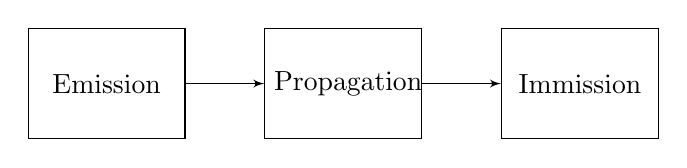
\begin{tikzpicture}[auto, node distance=1cm,>=latex']
\tikzset{
block/.style    = {draw, shape=rectangle, fill=white, minimum height=4em, minimum width=5em, text width=5em, align=center},
}
    % Main nodes
    \node [block]                       (emission)      {Emission};
    \node [block, right=of emission]    (propagation)     {Propagation};
    \node [block, right=of propagation]   (immission)         {Immission};

    % Main edges
    \draw [->]  (emission)      --  (propagation);
    \draw [->]  (propagation)   --  (immission);

\end{tikzpicture}
  \caption{Overview.}
  \label{fig:implementation:overview}
\end{figure}

The tools mentioned in \ref{sec:theory:auralisation:software} as well as other
general-purpose languages were considered for the implemention.
% TODO further motivation

The auralisation tool was implemented mostly in Python 3.5 \cite{Python} and
Cython \cite{Behnel2011,Cython}. Extensive use was made of the
Numpy\cite{VanderWalt2011,Numpy}, Scipy\cite{Scipy} and
Pandas\cite{Mckinney2010} libraries. A full implementation of the tool can be
found at \cite{Rietdijk2017d}.


\section{Propagation model}\label{sec:tool:propagation}

\subsection{Introduction}
% TODO remove turbulence from block diagram?
\begin{wrapfigure}{r}{0.3\textwidth}
  \centering
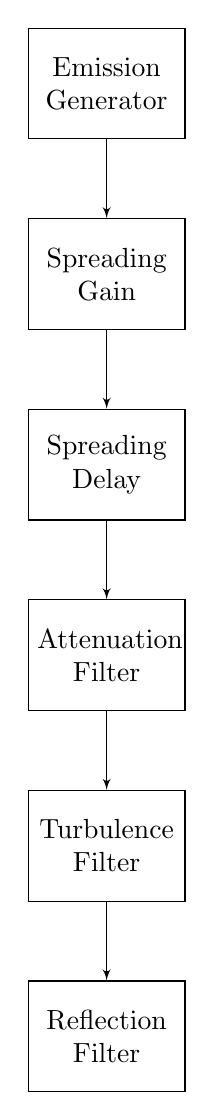
\begin{tikzpicture}[auto, node distance=1cm,>=latex']
\tikzset{
block/.style    = {draw, shape=rectangle, fill=white, minimum height=4em, minimum width=5em, text width=5em, align=center},
}
    % Main nodes
    \node [block]                       (emission)      {Emission\\Generator};
    \node [block, below=of emission]    (spreading)     {Spreading\\Gain};
    \node [block, below=of spreading]   (delay)         {Spreading\\Delay};
    \node [block, below=of delay]       (attenuation)   {Attenuation\\Filter};
    \node [block, below=of attenuation] (turbulence)    {Turbulence\\Filter};
    \node [block, below=of turbulence]  (reflection)    {Reflection\\Filter};

    % Main edges
    \draw [->]  (emission)      --  (spreading);
    \draw [->]  (spreading)     --  (delay);
    \draw [->]  (delay)         --  (attenuation);
    \draw [->]  (attenuation)   --  (turbulence);
    \draw [->]  (turbulence)    --  (reflection);

\end{tikzpicture}
  \caption{Block diagram of the propagation model. These steps are performed for each propagation path and the resulting signals are summed.}
  \label{fig:propagation_block_diagram}
\end{wrapfigure}


% TODO convective amplification is a source motion effect, not propagation.
% Discuss in other section?
% Convective amplification is supported in the
% propagation model but was ignored here.

The propagation model covers sound propagation in the far field through a
homogeneous and isotropic atmosphere and takes into account geometrical
spreading, Doppler shift, atmospheric attenuation and the ground reflection.
Sound is modelled as rays and the propagation effects are implemented as signal
processing operations.

The following sections will describe each of the implemented propagation effects
in detail. To also demonstrate the different propagation effects, a fixed
situation is considered and propagation effects are added sequentially.

Figure \ref{fig:propagation_block_diagram} shows a block diagram of the steps
that are taken. Because of source motion all propagation effects are
time-variant. The order of the operation matters although some could be
exchanged. For operations that are distance-dependent, care should be taken to
consider the distance at the emission or retarded time. Divergence is computed
first. The Doppler-shift, a result of a change in propagation delay as function
of time, occurs between the source and the medium. The shifted frequencies are
then attenuated in the atmosphere. A reflection is modeled as a parallel path
with a filter representing the reflection coefficient. In case there is no
movement this filter may be considered part of the mirror source, however, as
movement is considered it needs to be placed after the Doppler-shift has been
applied.

Paper \ref{paper:turbulence} describes a model that was developed to include
scintillations, that is, fluctuations in the sound due to atmospheric
turbulence. That part is discussed in detail in Chapter \ref{chapter:turbulence}
and therefore not included in this Chapter.

% TODO explain situation - check noise signal!!
\subsection{Emission signal and scenario}
A simple emission signal is considered consisting of pink noise and several harmonic tones with a
fundamental frequency of \SI{2000}{\hertz}, both modelled as a monopole point
source at the same position. The broadband noise is the sum of 1/1-octave
band-pass filtered noise. The band-pass filters are \nth{8} order Butterworth
filters implemented as second-order sections\footnote{
Higher-order IIR filters can easily become unstable. A solution is to implement
the filter as a serial cascade of biquad or second-order sections, i.e., filters
with two poles and two zeros.}. Directivity is not included, and
there are no other signal strength variations either.

The \say{aircraft} moves at a height of \SI{200}{\meter} and with a
speed of \SI{100}{\meter\per\second} straight over the receiver.
The receiver is at a height of 1.7 meters and 8 meters next to the flight path.
Figure \ref{fig:implementation:propagation:emission} shows a spectrogram of the
emission signal. In the next sections propagation effects will be added sequentially
resulting in clear changes to the immission.

% \clearpage

\begin{figure}[H]
  \centering
  \includegraphics[]{../figures/generated/propagation/emission}
  \caption{Spectrogram of the immission. Because in this case we do not consider sound propagation this in facts corresponds to the emission of the aircraft as function of the orientation. The immission is stationary because an omni-directional source is considered and no other emission variations are modelled.}
  \label{fig:implementation:propagation:emission}
\end{figure}


\newpage
\subsection{Geometrical spreading}
Geometrical spreading causes a decrease in amplitude with distance due to
divergence and increase in propagation delay with distance due to the finite
speed of sound. Far field is assumed in which case the sound pressure at the
receiver $p_{\mathrm{rcv}}$ is given by the Green's function given in equation
\eqref{eq:theory:sound:green-free-field}. The emission signal $p_{\mathrm{src}}$
is computed at a fixed distance from the source $r_{\mathrm{src}}$. The sound
pressure at a receiver at distance $r_{\mathrm{rcv}}$ can be obtained by
rescaling the magnitude of the sound pressure of the emission signal with the
ratio of the distances
\begin{equation}
 p_{\mathrm{rcv}} = p_{\mathrm{src}} \frac{r_{\mathrm{src}}}{r_{\mathrm{rcv}}}
\end{equation}
This operation is implemented as a simple gain. Figure
\ref{fig:implementation:propagation:spreading} shows a spectrogram of the
immission when geometrical spreading is taken into account and applied to the
signal showed in Figure \ref{fig:implementation:propagation:emission}. Due to
the applied gain the sound pressure level is lower when the aircraft is farther
away, which is here at the start and the end of the sample.

\begin{figure}[H]
  \centering
  \includegraphics[]{../figures/generated/propagation/spreading}
  \caption{Spectrogram of the immission when the amplitude decrease due to geometrical spreading is included.}
  \label{fig:implementation:propagation:spreading}
\end{figure}

\subsubsection{Doppler shift}
The time-dependent propagation delay, which is relevant for the Doppler shift,
is taken into account by resampling the discretized sound pressure signal with a
Variable Delay Line. Since the signal is discrete and the delay is generally not
an integer multiple of the sample time, an interpolation scheme is required.

% TODO some of it needs to go to theory
As explained in section \ref{sec:theory:signal:resampling}, multiple
interpolation schemes exist, including Lanczos interpolation that was used for
auralisation as well \cite{Rietdijk2015, Pieren2015}. In this case a linear
interpolation scheme was chosen due to its simplicity and computational
performance \cite{Heutschi2014}. While linear interpolation can cause audible
artifacts, these are in the case of a broadband signal less pronounced than if
solely a tonal component is considered as was demonstrated in Figure
\ref{fig:theory:signal-processing:resampling}.

For a given sound travel time $\Delta t(t)$ from source to receiver, the non-integer sample index
$n_{e}$ of the signal $y[n_e]$ at the source time-axis is given as
\begin{equation}
 n_{e} = n_r - \Delta t (t) \cdot f_s
\end{equation}
where $f_s$ is the fixed sampling frequency and $n_r$ the integer sample index
of the signal at the receiver time-axis. Equation
\eqref{eq:theory:signal:resampling:interpolation-linear} can then be used for
applying the Doppler shift when using $n=\floor{n_e}$ and $\eta = n_e - \floor{n_e}$
where $\floor{n_e}$ corresponds to the floor function of $n_e$.
Furthermore, an emission time should exist and therefore there is the
requirement $\floor{n_e} >= 0$.

% The received signal value $y$ at index $n_e$ is then determined by
% \begin{equation}
%  y[n_e] = \left( 1 - n_e +  \floor{n_e} \right) \cdot y \left[ \floor{n_e} \right] + \left( n_e - \floor{n_e} \right) * y \left[ \floor{n_e} + 1 \right]
% \end{equation}
% where $\floor{n_e}$ corresponds to the floor function of $n_e$.
The sound travel time was computed with the speed of sound $c =
343.2 \sqrt{ \frac{T}{T_0} }$ where $T$ is the temperature during the event and
$T_0 = 293.15$ K the reference temperature.
Figure \ref{fig:implementation:propagation:doppler} shows a spectrogram of the
immission when the propagation delay is also considered. The Doppler shift is
clearly visible, especially when considering the tonal components.
The black part in the first couple of seconds represents zero signal and is due to the initial propagation delay.

\begin{figure}[H]
  \centering
  \includegraphics[]{../figures/generated/propagation/doppler}
  \caption{Spectrogram of the immission when the propagation delay, and thus the Doppler shift, is included as well. }
  \label{fig:implementation:propagation:doppler}
\end{figure}

\newpage
\subsection{Atmospheric attenuation} % TODO refer to theory
Atmospheric attenuation is accounted for by creating a time-variant filter of length $N_{aa}$.
A single-sided magnitude spectrum is calculated as
\begin{equation}
 \left| H_{aa} \right| = 10^{- d \alpha(f) / 20}
\end{equation}
where $d$ is the source-receiver distance in \SI{}{meter} and $\alpha(f)$ the
frequency-dependent attenuation coefficient in \SI{}{\decibel\per\meter} computed using
equation \eqref{eq:theory:sound:atmospheric-attenuation}.

% The air pressure, relative humidity, and temperature were recorded during the event.
The impulse response of a magnitude-only or zero-phase filter is non-causal and therefore in
order to create a causal filter a linear-phase filter corresponding to a 90
degrees rotation is added. The spectrum is real and even, and therefore the impulse
response is real and even as well. After convolving the signal with the designed
filter the first $N_{aa}/2$ samples were dropped to account for the delay caused
by the linear-phase factor.

Convolution was performed using a segmented convolution as explained in section
\ref{sec:theory:signal:convolution}. The filter length was 4096 samples and the
hop size 256 samples. Transitioning to the next impulse response was done
without smoothing because the difference in the impulse responses is relatively
small.

Figure \ref{fig:implementation:propagation:attenuation} shows a spectrogram of
the immission when atmospheric attenuation is included. A reference atmosphere
was considered.

\begin{figure}[H]
  \centering
  \includegraphics[]{../figures/generated/propagation/attenuation}
  \caption{Spectrogram of the immission when atmospheric attenuation is included as well.}
  \label{fig:implementation:propagation:attenuation}
\end{figure}

\newpage
\subsection{Ground reflection} % TODO refer to theory. Extend?
While the Image Source Method was implemented with image
receivers instead of image sources, only one additional path,
a ground reflection, was considered. Therefore, the implementation of the ISM
will not be treated any further.

The ground reflection is considered as a second propagation path using a mirror receiver.
% The implementation supports direction-dependent emission signals, but because we had only one emission...
For the ground reflected path the same emission signal was used as for the
direct path, thereby ignoring directivity of the sources. The reason why the directivity of
the source is ignored will become clear in the following sections.

A filter was included to take into account the transfer funtion of the ground.
For the ground reflection the plane wave reflection coefficient was used (eq. \eqref{eq:theory:sound:reflection:plane}) and the impedance $Z$ was
calculated using Delany and Bazley's one-parameter model (eq. \eqref{eq:theory:sound:impedance:db}).

Because aircraft are mostly overhead and at larger distances,
using the plane wave reflection coefficient should typically be sufficient.
However, when simulating noise sources at low elevation angles, the plane-wave
assumption is no longer valid and must be replaced by a model that takes into
account the reflection of spherical waves from a ground surface of finite
impedance \cite{Tuttle2014}. % TODO rewrite. Maybe move to theory

The scenarios considered were landings. Because the area around the airport
consists mostly of grass a flow resistivity of
\SI{2e5}{\pascal\second\per\meter\squared} was chosen. The filter length was
4096 samples and the hop size 256 samples.

Figure \ref{fig:implementation:propagation:reflection} shows a spectrogram of
the immission when a reflection on a hard ground was added. The additional path
clearly causes interference as can be seen from the bands in the Figure.
The effect of a hard and soft ground was demonstrated before in Figure \ref{fig:theory:sound:reflection:ground}.

\begin{figure}[H]
  \centering
  \includegraphics[]{../figures/generated/propagation/reflection}
  \caption{Spectrogram of the immission when a ground reflection is present. The Lloyd's mirror effect is clearly visible.}
  \label{fig:implementation:propagation:reflection}
\end{figure} % TODO text

\newpage
\subsection{Concluding remarks}
This section gave an overview of the propagation model that was implemented in
the auralisation tool. The propagation effects that were considered were
implemented as signal processing operations. The model that was implemented
could now be used to investigate how properties of the atmosphere, boundaries
and the geometry, affect sound propagation.

After taking into account sound propagation an immission signal is obtained that
already starts to sound like an aircraft. However, thus far a simple emission
signal consisting of some noise and several tones was considered. The next
section presents a method to obtain a more accurate airplane emission signal.

%
%
%
%
% TODO: OLD PART
%
%
% Figure \ref{fig:propagation_model_propagation_model} represents a block
% diagram of the steps that are taken. The steps are taken for every
% source-(mirror)receiver combination.
%
%
% \begin{figure}[H]
%         \centering
%         \includegraphics[height=0.4\textheight]{../figures/propagation_model}
%         \caption{Block diagram of propagation model.}
%         \label{fig:propagation_model_propagation_model}
% \end{figure}
%
%
%
% \subsection{Attenuation due to spreading}
%
% Geometrical spreading
% \begin{equation}
%  p_t = p_0 \frac{r_0}{r_t}
% \end{equation}
%
% \newpage
% \subsection{Time delay and Doppler shift}
%
% The limited speed of sound causes a delay between receiving and emitting a signal.
% A common method to include this delay in a real-time implementation is to use a variable-delay line.   % Needs reference
% % This implementation is not real-time, resulting in more available options.
%
% % The time delay can be simulated using a variable delay line.
%
% Since the signal is discrete and the delay is generally not an integer multiple of the sample time, an interpolation scheme is required.
%
% \subsubsection{Linear interpolation}
% Initially, linear interpolation was used.
% For a given sound travel time $\Delta t(t)$ from source to receiver, the index
% $k_{r}^{'}$ is given as
% \begin{equation}
%  k_{r}^{'} = k_e + \Delta t (t) \cdot f_s
% \end{equation}
% where $f_s$ is the sampling frequency.
% ......
%
% Figure \ref{} shows an example where linear interpolation was used to apply a Doppler shift.
%
% \missingfigure{Spectrogram of a Doppler shifted tonal component. The Doppler shift was applied by resampling the signal and using linear interpolation.}
%
% The Doppler shifted tonal component is clearly visible, however, strong artefacts are also visible and indeed audible.
% In practice, these artifacts are often masked by noise components but this however cannot be guaranteed.
%
% There are methods to reduce these artefacts. For example, upsampling the signal before resampling decreases the prominence of the artifacts.
% Another possibility is a different interpolation scheme.
%
% \subsubsection{Lanczos interpolation}
% Theoretically, the optimal reconstruction filter is a sinc filter. In practice
% only approximations of this filter can be used, and these approximations are
% generally achieved by windowing and truncating the sinc function. One of these
% approximations is the Lanczos filter or kernel, which is the sinc function
% windowed by another sinc function.
%
% The Lanczos kernel is given by
% \begin{equation}
%  L(z) = \begin{cases}
%          \textrm{sinc}(z) \textrm{sinc}(z/a), & \textrm{if} -a < z < a \\
%          0, & \text{otherwise}
%         \end{cases}
% \end{equation}
% where $a$ is the size of the kernel. Consider now a signal with samples $s_i$
% for integer values of $i$ where sample $s_i$ corresponds to the sample at $t=i/f_s$.
% The value at retarded time $t'$ is then given by
% \begin{equation}
%  S(x) = \sum_{\floor{x} - a + 1}^{\floor{x} + a} s_i L(x-i)
% \end{equation}
% where $x$ is the sample at retarded time $t'$
% \begin{equation}
%  x = -t' + i
% \end{equation}
% The frequency shift depends on the change of propagation delay. Therefore, when source and receiver are relatively close to one another, the method is most sensitive to uncertainties in source position and speed of sound.
%
% \missingfigure{Spectrogram of a Doppler shifted tonal component. In this case the Doppler shift was applied by resampling the signal and using Lanczos interpolation. The artefacts are clearly less pronounced as those present in figure \ref{}}
%
% \missingfigure{Spectrogram of auralisation}
%
% \newpage
% \subsection{Atmospheric attenuation}
% The atmospheric attenuation coefficient $\alpha$ in dB/km is calculated according to ISO 9613-1 \cite{ISO9613-1} as presented in \ref{sec:theory_sound_atmospheric_attenuation}.
%
% A single-sided spectrum is calculated as
% % Equation \ref{} is sampled to obtain an attenuation spectrum in dB/m and then multiplied with the current distance to obtain the actual attenuation.
% \begin{equation}
%  10.0^{- d \alpha(f) / 20}
% \end{equation}
% The spectrum is real and even, and therefore the impulse response is real and even as well. A non-causal zero-phase filter was designed.
%
%
%
% The attenuation spectrum is converted to an impulse response using the IFFT.
% Because the attenuation is distance-dependent and the distance changes over time, the impulse response needs to be updated.
%
% The attenuation is applied by performing a convolution between the impulse responses and the input signal.
% The convolution is done by multiplying a matrix consisting of impulse responses with a vector representing the input signal.
% The impulse responses are stored in a sparse matrix to reduce memory consumption.
% Nevertheless, because of computational limitations, the impulse response describing atmospheric attenuation are determined for an $N$ amount unique distances.
%
% Since atmospheric absorption is frequency-dependent, care should be taken that
% one corrects for the Doppler shift first. Since a moving medium (due to wind) is not
% included in the propagation model, the time delay between source and receiver
% can be calculated directly, and the atmospheric absorption applied thereafter.
%
% \missingfigure{Spectrogram of auralisation}
%
% %
% % The attenuation coefficient for
% % pure tones $\alpha$ is calculated according to ISO 9613-1 \cite{ISO9613-1} in
% % the frequency domain. This attenuation, corresponding to a (single-sided) power spectrum in decibels, is converted to a double-sided amplitude spectrum
% % using
% % \begin{alignat}{2}
% %  a_{\alpha}[k] &= 10^{+ d \alpha}, && \quad 0 \leq k \leq N/2 \\
% %  a_{\alpha}[-k] &= a_{\alpha}[k], && \quad 1 \leq k \leq N/2-1
% % \end{alignat}
% % where $M$ is the amount of desired filter taps, $k$ the block index of discrete frequency $f_k$ and $d$ the source-receiver distance.
% % Note also the plus sign; in case of an auralization this sign would be negative but now we're interested in an amplification.
% % An impulse response is obtained by taking the IFFT of $M$ blocks. The small imaginary parts are discarded by taking the real part.
% % The filter is then made causal by rotating the impulse response with $M/2$ samples. A rectangular window was used.
% %
% % The attenuation is range-dependent and because of the aircraft movement the range varies with time. Within one recording there is a
% % maximum and minimum range. An $N$ amount of impulse responses are determined for
% % an $N$ amount of equispaced ranges.
% %
% % The attenuation is applied by performing a convolution between the impulse
% % responses and the input signal. The convolution is done in a rather naive way by multiplying a
% % Toeplitz matrix consisting of impulse responses with a vector representing the input
% % signal. The impulse responses are stored as a sparse array to reduce memory
% % consumption. No further operations were done regarding the impulse response transitions.
%
% \newpage
% \subsection{Atmospheric turbulence}
%
% - per octave band
%
% \missingfigure{Spectrogram of auralisation}
%
% \newpage
% \subsection{Reflections and shielding}
%
% In an urban environment reflections and shielding play a role.
%
% Hard surfaces except possibly the ground.
% Surfaces relatively smooth considering wavelength. Specular reflections are assumed.
%
% Considering the large distances compared to the wavelengths the waves can likely
% be assumed to be plane and a plane-wave reflection coefficient can be used. Then
% again, the increased computational effort of using a spherical reflection
% coefficient is negligible.
%
% \missingfigure{Spectrogram of auralisation}
%
% Using the image source method mirror receivers are determined.
% Their strength and effectiveness is determined every $N$ samples and the mirror receivers are sorted on strength.
% The strongest sources are selected.
%
% \newpage
% \subsection{Inverse propagation model}\label{sec:propagation_model_reverse_propagation_model}
% Based on this propagation model an inverse propagation model was developed.
% The inverse propagation model is used to calculate back to the source in order to determine emission characteristics.
%
% Figure \ref{fig:propagation_model_reverse_propagation_model} shows a block
% diagram of the steps taken in the reverse propagation model.
%
% A likely significant error that is being made is that the ground effect is
% still included.
%
%
% \begin{figure}[H]
%         \centering
%         \includegraphics[width=0.4\textwidth]{../figures/reverse_propagation_model}
%         \caption{Block diagram of reverse propagation model. A sound recording
% is used in conjunction with detailed flight path information. Spherical
% spreading, atmospheric absorption, and the Doppler shift are undone, resulting
% in a source signal.}
%         \label{fig:propagation_model_reverse_propagation_model}
% \end{figure}


\section{Backpropagation and emission synthesis}\label{sec:tool:synthesis}

\subsection{Introduction}
The previous section treated the propagation model of the tool. In order to
simulate the audible sound of aircraft an emission signal is needed. Thus far a
simple signal consisting of noise and a tone was considered. This section
describes a method to create an emission signal from features derived from
recordings. An auralisation or pseudo-recording at a receiver position can then
be created by propagating the signal using the propagation model. Figure
\ref{fig:tool:backpropagation:introduction:block-diagram} shows a block diagram
of the steps that are treated in this section.

\begin{figure}[H]
  \centering
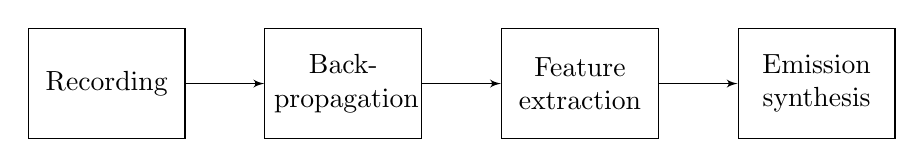
\begin{tikzpicture}[auto, node distance=1cm,>=latex']
\tikzset{
block/.style    = {draw, shape=rectangle, fill=white, minimum height=4em, minimum width=5em, text width=5em, align=center},
}
    % Main nodes
    \node [block]                       (recording)     {Recording};
    \node [block, right=of recording]   (backprop)      {Back-\\propagation};
    \node [block, right=of backprop]    (feature)       {Feature\\extraction};
    \node [block, right=of feature]     (emission)      {Emission\\synthesis};
%     \node [block, right=of emission]    (auralisation)  {Auralisation};

    % Main edges
    \draw [->]  (recording)     --  (backprop);
    \draw [->]  (backprop)      --  (feature);
    \draw [->]  (feature)       --  (emission);
%     \draw [->]  (emission)      --  (immission);

\end{tikzpicture}
  \caption{Block diagram of the backpropagation, synthesis and auralisation method.}
  \label{fig:tool:backpropagation:introduction:block-diagram}
\end{figure}

% An automated procedure was developed to a) backpropagate from source to receiver
% in time-domain and b) analyze the resulting signal to extract features that could be
% used in the development of an emission model or to directly resynthesise the
% emission.

% \subsection{Measurement data}

For the emission synthesis a signal is generated that is based on measurements
that were made for the sonAIR project as described in section
\ref{sec:introduction:sonair}. Figure \ref{fig:figure_trajectory} shows an
overview of the airport, the trajectory and the receiver of the events
considered. Aircraft took off and their height steadily increased from 30 to 260
meters.

% For the data presented measurements from only a single microphone
% were used, situated at a height of 4 meters.


% For the development of the sonAIR model \cite{Zellmann2016} sound recordings
% were made for a large amount of events nearby Z\"{u}rich Airport
% \cite{Zellmann2013}. Along with the sound recordings the position of the
% aircraft was registered and for a subset of the events more detailed information
% was obtained as well, like e.g. thrust settings. Recordings were made at
% multiple positions simultaneously, allowing to determine the directivity of the
% noise components.

\begin{figure}[H]
  \centering
  \includegraphics[width=0.3\textwidth]{../figures/manual/auralisation-paper/figure_trajectory}
  \caption{Overview of the airport, trajectory and the receiver. The receiver
(green dot) is situated slightly north of the trajectory, almost straight underneath the
trajectory.}
  \label{fig:figure_trajectory}
\end{figure}


\subsection{Backpropagation}
An automated procedure was developed to backpropagate from receiver to source in
time-domain. The procedure assumes there is only one propagation path,
the direct path, and that the aircraft can be considered a point source.
As shown in Figure \ref{fig:backpropagation_block_diagram}, the
backpropagation algorithm undoes atmospheric attenuation, the Doppler shift, and
geometrical spreading (magnitude) in that specific order, and using the methods as
described in the previous section.
% A recording is taken, and assuming there were no reflections, the atmospheric attenuation and spherical spreading were undone.
Because only the direct path was considered all parameters that were used in the
backpropagation were based on values corresponding to that path.

\begin{figure}[H]
  \centering
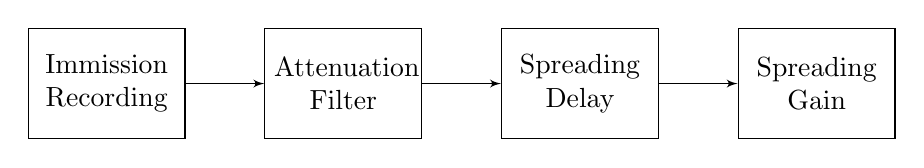
\begin{tikzpicture}[auto, node distance=1cm,>=latex']
\tikzset{
block/.style    = {draw, shape=rectangle, fill=white, minimum height=4em, minimum width=5em, text width=5em, align=center},
}
    % Main nodes
    \node [block]                       (immission)     {Immission\\Recording};
    \node [block, right=of immission]   (attenuation)   {Attenuation\\Filter};
    \node [block, right=of attenuation] (delay)         {Spreading\\Delay};
    \node [block, right=of delay]       (spreading)     {Spreading\\Gain};

    % Main edges
    \draw [->]  (immission)     --  (attenuation);
    \draw [->]  (attenuation)   --  (delay);
    \draw [->]  (delay)         --  (spreading);

\end{tikzpicture}
  \caption{Block diagram of the backpropagation model. These steps are applied sequentially to a recording in order to obtain a signal in time-domain that corresponds to the emission of the aircraft.}
  \label{fig:backpropagation_block_diagram}
\end{figure}

Application of the backpropagation algorithm results in a time-domain signal
that corresponds to the emission of the aircraft. The emission includes the
effect of convective amplification, i.e., the directivity effects due to source
motion.

The influence of the ground reflection is non-negligible. A soft ground is still
relatively hard and therefore a -3 dB correction was applied. Ideally, a
microphone on the ground was used, but the dataset that was available consisted
of recordings at a height of 4 meters.

Figures \ref{fig:recording} and \ref{fig:backpropagated} show spectrograms of
respectively the recording and of the signal that was backpropagated. The signal
after backpropagation is shorter than the recording due to lack of aircraft
position information during the initial propagation delay.
Aside from small variations the tonal components remain constant in frequency
over time in Figure \ref{fig:backpropagated}. The variations are caused
by uncertainties in the measured position of the aircraft and thus the estimated
propagation delay.


\begin{figure}[H]
  \centering
  \includegraphics[]{../figures/generated/recording-to-auralisation/recording}
  \caption{
    Spectrogram of a recording of an A320. Clearly visible are the
    Doppler-shifted tones and the peaks due to atmospheric turbulence.
    Interference between direct and reflected path acts as a Comb filter resulting
    in an acoustical Lloyd's mirror-effect, which can be seen here at lower
    frequencies. The most powerful tone corresponds to the blade passing frequency
    of the fan. The other tones are Buzz-Saw tones.}
  \label{fig:recording}
\end{figure}

\begin{figure}[H]
  \centering
  \includegraphics[]{../figures/generated/recording-to-auralisation/reverted}
  \caption{Spectrogram of the recording shown in Figure \ref{fig:recording} after backpropagation to the source. The Doppler-shift has mostly been removed. Artifacts like the mirror-effect and amplitude modulations due to atmospheric turbulence remain.}
  \label{fig:backpropagated}
\end{figure}

\subsection{Feature extraction}
Spectral modelling synthesis was chosen as emission synthesis strategy. With
spectral modelling synthesis a signal is generated as a superposition of tones
and bandpass-filtered noise.
% In order to synthesise the emission of the aircraft
% We're interested in entirely synthesizing the emission of the aircraft and chose to use
% spectral modelling synthesis, that is, a method where a signal is generated
% through a superposition of sines and noise.
Therefore, a method is needed to extract from the backpropagated recordings the
frequency, phase, and level of the tones, as well as the level of the noise as
function of frequency. This section presents a method that was developed for
extracting these features.

The situations considered are landings, and therefore the tonal components in
the spectra are not only the blade passing frequency of the fan and its
harmonics, but also \say{Buzz-Saw} tones. The common denominator of the
frequencies of these components is the frequency at which the engine shaft
rotates.

\subsubsection*{Motivation for method}
The events considered are short, typically less than 30 seconds, and their
spectra vary considerably over time due to directivity of the source. Thus, in
order to get a sufficiently good directivity resolution, a high temporal
resolution is needed, and that limits the possibility to average over time. The
frequency resolution, however, also matters. The emission may contain Buzz-Saw
harmonics with a fundamental frequency below 100 Hz. While that gives some
freedom for using a lower frequency resolution, first the actual tonal
components need to be detected and thus distinguished from the broadband noise.

While already corrected for in the backpropagation, the Doppler shift may make
it difficult connecting obtained frequency-components at one step to those
obtained the step later. Therefore, frequency-tracking algorithms were
considered \cite{Lampert2010}, notably Hidden Markov Models. Due to their
complexity such solutions were not pursued further.

Tone-detection in the frequency-domain is in its simplest form a matter of peak
detection for which a range of algorithms is known. However, a robust algorithm
is needed that can distinguish between the tonal components and broadband noise
peaks.

Initially, the complex cepstrum\footnote{The complex cepstrum is defined as
$c[n] = F^{-1}\left\{\log_{10}{\left( F \left\{x[n]\right\} \right)}\right\}$.}
was used to determine the fundamental frequency of the Buzz-Saw harmonics
(Paper \ref{paper:euronoise2015}). The method was reliable for determining the
fundamental frequency. Because all the tonal components considered are multiples
of this fundamental frequency, all their frequencies would then be known as
well. Unfortunately, the frequency-resolution, or more precisely the
quefrency-resolution, was not high enough to reliably predict the frequency of
the high-frequent components.

\subsubsection*{Tone-seeking algorithm}
Annex C of ISO 1996-2:2007 \cite{ISO1996-2_2007} describes an objective method
for assessing the audibility of tones in noise and a significant part of the
method describes a tone-seeking algorithm. The tone-seeking algorithm works in
frequency-domain on a narrowband power spectrum. An estimate of the narrowband
spectrum is obtained using Welch's method. The time signal is split in chunks, a
Hanning window is applied to each chunk, and a periodogram is determined for
each chunk. Finally, linear averaging over the chunks results in Welch's
estimate of the power spectral density.

According to the standard an A-weighted signal should be used. Because the
frequencies of the tonal components are of interest, and not their audibilities,
an unweighted signal is considered instead. Furthermore, in order to obtain an
accurate estimation an averaging-time of one minute is required, however, this
could not be done as explained.

The tone-seeking algorithm first determines noise pauses, which are local maxima
with a probability of a tone. The next step is to assess whether tones exist in
these noise pauses. Each frequency bin or line is assigned a label indicating whether
it is part of a tone or whether it is masking noise.
% The tone-seeking algorithm was implemented according to the standard.

The power of the lines that are part of a tone are integrated. A correction is
made for the masking noise contributions to those lines by estimating their
contribution from a regression through the lines marked as noise within a
portion of the critical band\footnote{A critical band is the bandwidth of a
filter created by the cochlea, the auditory part of the inner ear.} around the
centerfrequency of the tone.

\subsubsection*{Extension}
The tone-seeking algorithm is capable of detecting many of the tonal components
but not all of them. Because the tones of interest are all multiples of a
fundamental frequency the goal is to determine this fundamental frequency
sufficiently accurate. The assumption was therefore made that all tones found by the
tone-seeking algorithm from the standard were harmonics and that the fundamental
frequency was within a specified range.
The fundamental frequency is then given
\begin{equation}
 f_{0} = \mathrm{gcd}\left(f_1, f_2, \dots, f_n \right)
\end{equation}
where $\mathrm{gcd}$ is the \emph{greatest common divisor} (Paper \ref{paper:internoise2016}).
Implementations of the $\mathrm{gcd}$ operator attempt to find an exact solution.
Due to errors in the estimation of the frequency of the tones and because some tones are
not harmonics, an exact solution does not exist. Given an initial estimate of
the fundamental frequency, one could define an error as the sum of the squared
deviation between the target order of the harmonics and the actual estimated
order
\begin{equation}
 e = \sum_{i=0}^{n} \left( \frac{f_i}{f_0} - \mathrm{round}\left(\frac{f_i}{f_0}\right) \right)^2
\end{equation}
An estimate of the fundamental frequency is obtained by minimising this error.

The tone-seeking algorithm is first ran to detect tonal components and obtain their centerfrequencies.
% TODO bandwidth!
Then, a fundamental frequency estimation is done. Next, the frequency lines
within ??? hertz are added as noise pauses.
The tone-seeking algorithm determines for these lines again whether they could
be tones and outputs levels for all tonal components.
Finally, the masking noise lines were integrated in \nicefrac{1}{6}-octaves.


% An earlier version of the algorithm did not use the $\mathrm{gcd}$ in
% combination with the optimisation algorithm but instead determined the
% fundamental frequency using the complex cepstrum (Paper ).
% While it was possible to reliably determine the fundamental frequency with the
% complex cepstrum, the value which was obtained was not sufficiently accurate
% for determining higher harmonics.

% In the method as described in Annex C of ISO 1996-2:2007 each spectral line is
% assigned a label, e.g. whether the line is part of a tone or noise. Tones
% typically have a bandwidth and can therefore, depending on the frequency
% resolution, be spread over multiple lines. In order to compute the level of a
% tone, the spectral lines corresponding to that tone need to be integrated.

The bandwidth of the tonal components depends on various aspects, like frequency
or phase modulations at the source or during propagation, e.g. due to
atmospheric turbulence. The direct and reflected contribution are
Doppler-shifted slightly differently and that causes either double peaks or a
single broader peak. But also averaging time and window shape play a role.

% The center frequencies of the tonal components obtained with the enhanced method
% were fed back in the method of the standard to obtain labels for each spectral
% line and to compute the levels of the tones and the noise.

% The lines that were assigned noise were integrated into \nicefrac{1}{6} octaves and for each
% fractional octave its level was kept.

For the feature extraction two seconds windows were used, without overlap.
While a short window decreases frequency resolution and precision of the
features, a short
window was required in order to provide temporal resolution of the features.
A 2 seconds window proved to be a good balance between temporal resolution
and frequency resolution. A value for the phase could not be obtained because
the signal was too noisy.

% For the development of an emission model it is expected that
% the uncertainties could be reduced through ensemble averaging. % TODO include this?

\subsection{Emission and immission synthesis}\label{sec:tool:synthesis:synthesis}
% As mentioned before the emission was synthesised using spectral modelling
% synthesis.
With the extracted features, which were obtained as function of time and at
several receiver positions, it is possible to develop an emission model that
takes into account directivity of the spectral components. Such emission model
would then output input for the SMS synthesiser and the created emission signal
would be propagated to a receiver a location.

An important question to ask is whether the described methodology of extracting
features, synthesising an emission signal and propagating it would result in
plausible auralisations. For example, it could be possible that the chosen
synthesis strategy and features cannot reproduce certain characteristics in the
sound. Therefore, the next chapter describes a comparison between auralisations
and recordings with the auralisations based on recordings.

For a specific event and receiver, the immission was backpropagated and features
were extracted. These features were used to re-synthesise the emission. The
emission signal was propagated to the receiver, and a direct path and a single
reflection were considered. The assumption was made that the emission is
identical for the emission angles corresponding to direct and reflected path.

The feature extraction method provided frequencies and levels of tonal
components as function of time. Variations in the frequencies as function of
time could be observed, but with a two second window that would result in only
few data points. Variations in frequency were therefore ignored and computed was an
average value for the fundamental and each of the harmonics.

As mentioned in the previous section, values for the phase of the tones could
not be obtained, and therefore values had to be chosen. Because the harmonics
are \say{Buzz-Saw} noise, a phase corresponding to a sawtooth signal was
initially assumed. Participants in a preliminary test found the simulations
sound metallic compared to the recordings (Paper \ref{paper:internoise2016}). Therefore, the
assumption was made that the initial phase relation between the Buzz-Saw tones
was entirely lost and could therefore be chosen randomly. In that case the
probability distribution would be uniform.

Figures \ref{fig:synthesis} and \ref{fig:auralisation} show spectrograms of
respectively the emission synthesis and the auralisation at the receiver.

\newpage
\afterpage{
\begin{figure}[H]
  \centering
  \includegraphics[]{../figures/generated/recording-to-auralisation/synthesis}
  \caption{Emission synthesis of the aircraft. Inputs to the emission synthesiser were obtained by applying the feature-extraction algorithm to the signal shown in Figure \ref{fig:backpropagated}. The level of the tonal components vary over time. The blade passing frequency is not clearly visible because the determined level of the tone was underestimated.}
  \label{fig:synthesis}
\end{figure}


\begin{figure}[H]
  \centering
  \includegraphics[]{../figures/generated/recording-to-auralisation/auralisation}
  \caption{Auralisation of the event shown in Figure \ref{fig:recording} .
  The Doppler-shifted tones and the mirror-effect are clearly visible. The Doppler-shifted tones are not very smooth. This is due to fluctuations in the aircraft position due to uncertainties.}
  \label{fig:auralisation}
\end{figure}
}


%
%
%
%
%
%
%
%  TODO: BELOW IS OLD STUFF
%
%
% \section{Emission model}
%
% The emission model describes the emission of aircraft. In this section we discuss the development of the model as well as the eventual implementation.
%
% As described in \ref{sec:theory_aircraft_emission_models} several emission models exist.
%
% What is needed for the auralizations is a model that can describe tonal and noise components.
% The models referred to all predict sound levels in fractional-octaves.
%
% Therefore, we will now try to extract the relevant features using an automated method. The method is roughly as follows:
%
% \begin{enumerate}
%  \item Backpropagate from source to receiver in time-domain, undoing the Doppler shift, atmospheric attenuation and spreading. The ground effect is ignored for now. We now have a signal that roughly corresponds to what is emitted from the airplane.
%  \item Determine fundamental frequency. An aircraft spectrum consists mostly of noise and tones, which are mostly harmonics. Knowing the fundamental frequency, allows you to determine the power of not only the fundamental, but also of each harmonic.
%  \item And that is the final step. Determine power of the tones, and consider the rest of the spectrum as noise.
% \end{enumerate}
%
%
%
% \subsection{Empirical model}
% In the sonAir project aircraft landings and take-offs were recorded.
%
% \subsubsection{sonAir data acquisition}
%
% \newpage
% \section{Backpropagation in time-domain}
% To backpropagate in time-domain an inverse propagation model was developed that is based on the propagation model explained in \ref{}.
% The inverse propagation model undoes the intensity loss due to geometrical spreading, as well as the propagation delay that causes the Doppler shift.
% Furthermore, the inverse propagation model corrects for atmospheric attenuation.
% One effect the inverse propagation model cannot undo is the ground effect.
%
%
% \subsubsection{Limitations of the method}
%
%
% \subsubsection{Ground effect}
%
%
%
%
% Now that some of the propagation effects have been undone we have a signal that roughly corresponds to as if you would fly along with the aircraft, and rotate around it.
%
%
% \missingfigure{Spectrum of the recorded signal after backpropagating in time-domain.}
%
% \missingfigure{Power spectrum of the reverted signal.}
%
% \newpage
% \subsection{Determine fundamental frequency}
% To determine the fundamental frequency in an automated and reliable way, several methods were tried.
%
% \subsubsection{Using complex cepstrum}
%
% Using the complex cepstrum it was possible to obtain an accurate estimate for the fundamental frequency. However, the estimate proved not accurate enough to determine the higher-frequency harmonics.
% Since the frequency of an harmonic is the fundamental multiplied by the order, any inaccuracy in the estimate is multiplied as well. For harmonics around the blade passing frequency and up the error was generally too big.
% Therefore, another method was sought.
%
% \missingfigure{In the complex cepstrum a peak can be found that corresponds to the fundamental frequency.}
%
% \subsubsection{Estimate fundamental from determined tones}
% Estimating the fundamental frequency directly from a spectrum result in an inaccurate estimate. However, when using multiple harmonics, and especially higher order harmonics, the estimate in the error can drop significantly.
%
% \begin{enumerate}
%  \item Determine frequency of harmonics using a tone-seeking algorithm.
%  \item Estimate fundamental frequency given the frequencies of the harmonics.
% \end{enumerate}
%
% An example of a simple tone-seeking algorithm is one that checks when, in the estimate of the power spectrum, the steepness gets above or below a certain threshold. When the threshold is passed twiced - the second sweep in opposite direction - a tone might be present.
% ISO 1996-2:2007 Annex C provides an objective method for assessing the audibility of tones in noise, and part of the method is a tone-seeking algorithm that does exactly this. Aside from the tone-seeking algorithm, the objective method also provides a method for assessing the tones, including estimating their power.
%
% \fbox{\begin{minipage}{0.5\textwidth}
% A method to verify whether audible tones are present in a signal is provided in ISO 1996-2:2007 Annex C. Based on the prominence of tones, the method also provides recommended level adjustments.
% \begin{enumerate}
% \item Find preliminary noise pauses.
% \item Search for tones in noise pauses.
% \item Put a critical band on the centerfrequency of the tone, and determine the tone strength, masking noise level and finally the tonal audibility.
% \item The final tonality adjustment is determined by the tone with the highest tonal audibility.
% \end{enumerate}
% \end{minipage}}
%
% \missingfigure{Tones and critical bands assessed using an implementation of ISO 1996-2:2007 Annex C}
%
% Using a tone-seeking algorithm like the one provided by the standard, one can obtain estimates of the frequencies of tonal components. However, it is not yet known which harmonic order the tone has, or in fact whether it is a harmonic at all.
% Even so, assuming the tones are all harmonic and exact, then the fundamental frequency $f_{0}$ would be the greatest common divisor of the harmonics $f_i$
% \begin{equation}
%  f_{0} = \mathrm{gcd}\left(f_1, f_2, \dots, f_n \right)
% \end{equation}
% Implementations of the $\mathrm{gcd}$ attempt to find an exact solution. However, due to errors in the estimate of the tones (because of a limited frequency resolution) and because some tones are not harmonics, an exact solution would not exist.
% Given an initial estimate of the fundamental frequency, one could define an error as the sum of the squared deviation between the target order of the harmonics and the actual (inaccurate) order
% \begin{equation}
%  e = \sum_{i=0}^{n} \left( \frac{f_i}{f_0} - \mathrm{round}\left(\frac{f_i}{f_0}\right) \right)^2
% \end{equation}
% The fundamental frequency is obtained by minimizing this error. Without constraining the fundamental frequency, incorrect estimates are likely to be obtained. For example, an estimate of the fundamental that is half the actual frequency would fit. And a lower frequency, would also result in a smaller error, causing a preference for a very low-frequency fundamental.
% In our case, we know that the fundamental frequency is generally between 60 and 80 Hz, eliminating both problems.
%
% However, it might still happen that several tones are estimated to be the same harmonic - which is obviously incorrect - and thereby increasing the error in the estimate of the fundamental.
% This can be prevented by checking all combinations with each combination consisting of only unique harmonics. The combination that minimises the error is kept.
%
% The eventual method is:
% \begin{enumerate}
%  \item Estimate frequencies of tones using the tone-seeking algorithm described in ISO 1996-2:2007 Annex C.
%  \item Estimate which harmonic order the tones are.
%  \item Obtain initial estimate of fundamental frequency from the estimated tone frequencies and harmonic orders using a least-squared method. An error is defined as the sum of the absolute deviation between frequency estimate given by 1, and the harmonic order multiplied with the fundamental frequency.
%  \item It might occur that multiple tones would seem to correspond to the same harmonic. This is not possible and should be prevented.
%  \item Therefore all combinations of harmonic order estimates are checked. The result with the smallest error is the final result of the algorithm.
% \end{enumerate}
%
% \newpage
% \subsection{Determine features}
% With the estimate of the fundamental frequency, we also know what the frequencies
% of the harmonics are. The ISO method not only provides an algorithm to determine
% tones, but also a method for assessing them.
%
% We now feed the estimated harmonics back into the ISO method, setting noise
% pause starts and ends at $f_i -/+ f_c/8$. The tone level and bandwidth is is
% determined for each tone, overriding the requirements that frequency lines
% within 6 dB of the maximum should be present, and that the bandwidth should be
% less than 10\% of the critical band.
%
% The frequency of each of these tones is kept as well. The noise lines are
% integrated per fractional-octave.
%
% \begin{table}[h]\centering
%   \caption{Overview of the features.}
%     \begin{tabular}{ | l | l | l | p{5cm} |}
%     \hline
%     Component & Feature & Time-variant \\ \hline
%     Tone & center frequency & yes \\ \hline
%     Tone & bandwidth & yes \\ \hline
%     Tone & sound pressure level & yes \\ \hline
%     Noise & fractional-octave center frequency & no  \\ \hline
%     Noise & fractional-octave band designator & no  \\ \hline
%     \end{tabular}
% \end{table}
%
% \subsubsection{Noise floor}
% The signal-to-noise ratio is dependent on range and thus time. For the samples that were analysed, the noise floor took over at between 8 and 12 kHz.
% For this reason features were only extracted below 8 kHz.
%
% % Knowing the bandpass
% % Furthermore, ISO 1996:2-2007 describes for each frequency line whether it is consider a tone, noise, or neither.
% % This signal can be used to extract relevant features.
% % Many methods exist to detect and track tonal components.
% % ISO 1996-2:2007 Annex C provides an objective method for assessing the audibility of tones in noise.
%
%
% \newpage
% \subsection{Verify features through an auralization}
% Before analysing the features and developing an emission model from them, its important to ask
% the following question. Are these features sufficient to create a realistic
% emission signal? Or, even better, are these features, taking into account the
% developed propagation model, providing a realistic signal at the receiver? Does,
% what you hear, really sound like an aircraft? That is after all the aim.
%
% To verify whether the features contain enough information in order to create a
% plausible auralization, an emission signal was constructed from the features,
% and propagated to the receiver that was used for the measurement.
%
% \subsubsection{Synthesis of emission signal}
% The features that were obtained every second were linearly interpolated to a sample frequency of 22 kHz and were smoothed by applying a rolling mean in both directions.
% The only exception were the frequencies of the harmonics, for which average values were taken. % EXPLAIN!!
% The components are added together resulting in the final signal.
% Figure \ref{} shows a spectrogram of a synthesized emission signal.
%
% \missingfigure{Spectrogram of synthesized emission signal}
%
% \missingfigure{Unweighted sound pressure level as function of time. Fast time-weighting was applied.}
%
% \newpage
% \subsubsection{Signal at receiver}
% We now try to model the propagation of the original event as accurate as
% possible. A virtual receiver is positioned where the real receiver was. Below
% the receiver a flat ground is modelled, disregarding small height differences
% that are present in reality. The ground is modelled to be grass entirely, with
% the impedance calculated using ........
%
% A moving point source follows the original trajectory. The synthesized emission
% signal is now fed directly into the propagation model and is used for both the
% direct path as well as possible reflected paths. The virtual source is modelled
% as a omni-directional source because the synthesis already includes the gain
% adjustment due to source directivity. However, this gain is for a fixed set of
% angles i.e., the angles corresponding to the direct path. For the reflected
% paths the directivity would in reality be slightly different but this effect
% cannot be included in this verification.
%
% Included propagation effects were....
%
% Figure \ref{} shows a spectrogram of a verification auralization as well as a spectrogram of the original recording and figure \ref{} shows the A-weighted sound pressure level as function of time for both.
% \missingfigure{Spectrogram of synthesized emission signal and recording.}
% \missingfigure{A-weighted sound pressure level as function of time. Fast time-weighting was applied.}
%
%
% \newpage
% \subsection{Model}
%





\chapter{Propagation in a turbulent atmosphere}\label{chapter:turbulence}\todo{From paper. Rewrite}

\section{Introduction}

% TODO: rewrite paragraph from paper
In an outdoor situation, spatial and temporal variations in temperature and wind
velocity cause small changes in the refractive index. As waves pass through the
atmosphere, the index-of-refraction variations in effect cause scintillations,
i.e. fluctuations in the received intensity of the wave. Scintillations affect
both sound and electromagnetic waves. They are a major limitation for
astronomical observations using Earth-based telescopes and also reduce
performance of wireless communication systems. Scintillations can also be
noticed when hearing sound emitted by a source at a large distance, like for
example by an aircraft or distant windturbine \cite{Heutschi2014}.

The fluctuations due to atmospheric turbulence can be clearly audible, and
therefore it is presumed that including scintillations in auralisations
increases their perceived realism.

The multiple scattering affects the phase of the signal as well as the
log-amplitude. In previous work a coherence factor was introduced that would
account for coherence loss due to phase \cite{Shin2006, Arntzen2014b,
Arntzen2014a}. Fluctuations due to turbulence have also been included in
auralisations by simulating the amplitude modulations that were observed in
measurements \cite{Heutschi2014, Minard2016}.

% TODO: rewrite paragraph from paper
A method is presented to generate time series of sound pressure
fluctuations caused by line-of-sight propagation through a weakly turbulent
atmosphere. Novel in this field, the method includes both log-amplitude and
phase fluctuations. The presented method is based on \cite{Jurado-navas2006}
where it was used to predict the performance of wireless communication links,
and \cite{Forssen2000} where it was used to determine the influence of
turbulence on the performance of a barrier. The method was also
to increase the perceptual validity of auralisations
\cite{Rietdijk2014,Rietdijk2014a}.

\newpage
\section{Wave propagation in random media}

\subsection{Rytov approximation}
Variations in temperature and wind in both position $\mathbf{r}$ and time $t$ cause variations in the refractive index field $n(\mathbf{r},t)$.
We are interested in how these variations affect wave propagation and follow \cite{Ishimaru1997} and \cite{Jurado-navas2006}, but instead of electromagnetic waves, we consider sound waves.
We consider for now spatial variations only, and as a starting point we use the following Helmholtz equation %\cite{Ishimaru1997}
% Helmholtz equation is a stochastic differential equation % Because n(r) is a stochastic field
\begin{equation}\label{eq:helmholtz_without_fluctuations}
 \left( \nabla^2 + k^2 n^2(\mathbf{r}) \right) p(\mathbf{r})= 0
\end{equation}
with pressure $p$, wavenumber $k$, and refractive-index field
\begin{equation}\label{eq:refractive_index_field}
 n(\mathbf{r}) = n_0 + n_1(\mathbf{r})
\end{equation}
with mean value $n_0 = E[n(\mathbf{r})] = 1$ and first-order perturbation $n_1(\mathbf{r}) \ll 1$. Merging equations \eqref{eq:helmholtz_without_fluctuations} and \eqref{eq:refractive_index_field} results in
\begin{equation}\label{eq:helmholtz_with_fluctuations}
 \left( \nabla^2 + k^2 (n_0 + n_1(\mathbf{r}))^2 \right) p(\mathbf{r}) = 0
\end{equation}
For weak fluctuations, an approximation to equation \eqref{eq:helmholtz_with_fluctuations} for small $n_1$ is used.
The Rytov solution to equation \eqref{eq:helmholtz_with_fluctuations} is
\begin{equation}
 p = \exp{\left(\psi_0 + \psi_1 + \psi_2 + \dots \right)} = \exp{(\psi)}
\end{equation}
where $\psi_0$ is the complex phase of the unperturbed wave in free space, and $\psi_1$ and $\psi_2$ respectively first-order and second-order complex phase perturbations.

We are interested in the effect of first-order perturbations $n_1$, on the sound pressure,
and therefore write $\psi = \psi_0 + \psi_1$. The refractive index $n$ is written in terms of
an average $\langle n \rangle$ and fluctuation $n_1$, with
\begin{equation}
 \delta n = (1 + n_1)^2 -1 = 2 n_1 + n_1^2
\end{equation}
As derived in \cite{Ishimaru1997}, $\psi_{1}$ satisfies the following integral equation
\begin{equation}
 \psi_{1}(\mathbf{r}) = \frac{1}{p_0(\mathbf{r})} \int_{V'} G(\mathbf{r}-\mathbf{r}') \left[ \nabla \psi_1 \cdot \nabla \psi_1 + k^2 \delta n  \right]  p_0(\mathbf{r}') dV'
\end{equation}
where $G(\mathbf{r}-\mathbf{r}')$ is the free field Green's function. By iteration a series solution can be obtained. For the first iteration we set $\psi_1 = 0$ inside the integral and obtain the first Rytov solution
\begin{equation}
 \psi_{10}(\mathbf{r}) = \frac{k^2}{p_0(\mathbf{r})} \int_{V'} G(\mathbf{r}-\mathbf{r}') \delta n(\mathbf{r}') p_0(\mathbf{r}') dV'
\end{equation}
where $p_0(\mathbf{r})$ is the unperturbed sound pressure field. %, $\mathbf{r}$ a
The sound pressure after the first iteration is then
\begin{equation}
 p (\mathbf{r}) = e^{(\psi_0 + \psi_{10})} = p_0(\mathbf{r}) e^{(\psi_{10})}
\end{equation}

The first-order complex phase perturbation $\psi_{1}$ can be understood as a sum of waves,
generated at various points $\mathbf{r}'$ throughout the scattering volume $V'$.
The strength of each of these waves is proportional to the product of the unperturbed field term ${p_0}$, and the refractive-index perturbation $\delta n$ at a point $\mathbf{r}'$ \cite{Jurado-navas2006}.

\subsection{Amplitude and phase fluctuations}
We now want to find expressions for the log-amplitude and phase fluctuations, and will use Rytov's first solution.
We approximate the refractive-index fluctuation as
\begin{equation}
 \delta n = 2 n_1 + n_1^2 \simeq 2 n_1
\end{equation}
and write
\begin{equation}\label{eq:complex_exponential}
 p(\mathbf{r}) = A(\mathbf{r}) e^{jS(\mathbf{r})},  \quad p_0(\mathbf{r}) = A_0(\mathbf{r}) e^{jS_0(\mathbf{r})}
\end{equation}
where $A$ and $S$ are respectively the amplitude and phase of the fluctuating field $p(\mathbf{r})$,
and obtain for the first order perturbations
\begin{equation}\label{eq:chi_and_S}
 \psi_1 ({\mathbf{r}}) = \chi + j S = \log{(A/A_0)} + j (S-S_0)
\end{equation}
In this expression $\chi$ and $S$ represent respectively the log-amplitude fluctuation and phase fluctuation.

By applying the central limit theorem to the first Rytov solution, it follows that the complex phase follows a normal probability distribution \cite{Jurado-navas2006}.
This is an important result to keep in mind when generating sequences of fluctuations.

\subsection{Amplitude and phase covariance}
The log-amplitude and phase fluctuations are considered to be the result of a
random temperature fluctuation field. A characteristic of a random function or
field is its correlation function \cite{Tatarskii1971}. The spatial correlation
function of a random field $f(\mathbf{r})$, as function of distance $\mathbf{r}=\mathbf{r}_2-\mathbf{r}_1$
between observation points $\mathbf{r}_1$ and $\mathbf{r}_2$, is defined as
\begin{equation}
 C(\mathbf{r}_1, \mathbf{r}_2) = \langle f(\mathbf{r}_1)  f(\mathbf{r}_2) \rangle
\end{equation}
In a homogeneous and isotropic random field the correlation function
$C(r)$ depends only on the distance $r = \lVert \mathbf{r}_2-\mathbf{r}_1 \rVert$ between the observation points and not the path $\mathbf{r}=\mathbf{r}_2-\mathbf{r}_1$ \cite{Salomons2001}.
Note that at this point, the atmosphere is assumed frozen in time, i.e., variations are only spatially, not temporal.

We would like to obtain expressions for the covariance functions of the
log-amplitude and phase fluctuations. A specific part of the turbulence spectrum
can be approximated with a Gaussian correlation function
\begin{equation}
 C_{\mu} = \langle \mu(r_1) \mu(r_2) \rangle = \sigma_{\mu}^2 e^{-x^2/L^2}
\end{equation}
where $\sigma_{\mu}^2$ is the variance of the dynamic refractive index,
$x=r_1-r_2$ the distance between two points in space and $L$ the correlation
distance or length \cite{Ishimaru1997}.

% \todo{Explain why we go from $x$ to $\rho$ and $d$, i.e., 2 dimensions.}
We shall now consider a line-of-sight situation where $d$ is the
distance between the source and a receiver pair along the wave propagation
direction, and $\rho$ the spatial separation of the receivers transverse to the
wave propagation direction.

If the correlation length $L$ is much smaller than the Fresnel zone size of the sound
$\sqrt{\lambda d}$, then the log-amplitude and phase variance scale with
$\sigma_{\chi}^2=\sigma_{S}^2 \sim k^2 d$
\cite{Ishimaru1997} and the variances of the fluctuations are given by \cite{Daigle1983}
\begin{equation}\label{eq:model_daigle}
 \sigma_{\chi}^2 = \sigma_{S}^2 = \frac{\sqrt{\pi}}{2} \sigma_{\mu}^2 k^2 d L
\end{equation}

For spherical waves the covariances of the fluctuations, $B_{\chi}(\rho)$ and
$B_{S}(\rho)$, normalized to their variances, are given by
\begin{equation}
 \frac{B_{\chi} (\rho)}{\sigma_{\chi}^2} = \frac{B_{S} (\rho)}{\sigma_{S}^2} = \frac{\Phi\left(\rho/L\right)}{\rho/L} = C_{sp}(\rho)
\end{equation}
where
\begin{align}\label{eq:gaussian_correlation}
 \Phi \left(\rho/L \right) &= \int_0^{\rho/L} \exp{\left(-u^2\right)} \mathrm{d} u  \\
 &= \frac{1}{2} \sqrt{\pi} \mathrm{erf}\left( \rho/L \right)
\end{align}
and $\mathrm{erf}$ is the error function.
The covariance functions of the fluctuations $B_{\chi}(\rho)$ and $B_{S}(\rho)$ are thus
\begin{equation}\label{eq:variances}
 B_{\chi} (\rho) = B_{S}(\rho) = \frac{\sqrt{\pi}}{2} \sigma_{\mu}^2 k^2 d L
\frac{\Phi(\rho/L) }{\rho / L}
\end{equation}
% according to Daigle's model.

Still assuming Taylor's hypothesis regarding frozen turbulence, we can perform a
space-to-time conversion of the correlation and covariance functions to obtain
$C(\tau)$ and $B(\tau)$ respectively. The turbulence correlation time is given
by
\begin{equation}
 \tau_0 = \frac{L}{v_{\bot}}
\end{equation}
and the transverse time lag by
\begin{equation}
  \tau = \frac{\rho}{v_{\bot}}
\end{equation}
where $v_{\bot}$ is the transverse speed, corresponding to e.g. the mean speed
at which the field is carried by the wind transverse to the wave propagation
direction.

In this paper we will continue to use the covariance for spherical waves and a
Gaussian spectrum, because the Gaussian spectrum is the simplest model to work
with and computationally least demanding, but the method can also be used with
covariance functions that describe other turbulence spectra, like e.g. the Von
Karman spectrum \cite{Ostashev2015}.

\subsection{Propagation in the turbulent atmosphere as a multichannel}
The fluctuations in the atmosphere are temporal and/or spatial. Therefore, to
model sound propagation of a signal $x(t)$ through such an atmosphere a
time-varying channel is necessary. The received signal $y(t)$ consists of a
line-of-sight contribution and additional contributions from scattering,
together forming a multichannel \cite{Jurado-navas2006}.
Ignoring beam spreading, we can write this as %The received signal can be written as the sum of $n$ channels
\begin{equation}
 y(t) = \sum_{n} \alpha_{sc_{n}}(t) x(t-\tau_n(t))
\end{equation}
where $\alpha_{sc_{n}}(t)$ is the time-varying scintillation sequence
representing the effect of the pressure fluctuations on the $n$th-multipath
component, and $\tau_n$ the propagation delay of the $n$th component relative to the propagation delay in an undisturbed atmosphere.
Assuming the spread in propagation delay over the channels is small compared to the inverse of the signal bandwidth, so that $x(t-\tau_n) \approx x(t - \tau(t))$, then
\begin{equation}
 y(t) = x(t - \tau(t)) \sum_n \alpha_{sc_{n}}(t)
\end{equation}
Because the attenuation is very similar for the different multipaths, we can write that
\begin{equation}\label{eq:generating_sequences_multiplicative}
 y(t) = x(t - \tau(t)) \alpha_{sc}(t)
\end{equation}
Therefore, the received signal is obtained by shifting the emitted signal $x(t)$ with a time-varying propagation delay $\tau(t)$, and multiplying the result with a time-varying gain $\alpha_{sc}(t)$.

\section{Generating sequences of scintillations}

\subsection{Design of scintillation sequence}
We will now design a sequence of scintillations and for that we need to know the
statistical distribution and power spectral density $|H_B(f)|^2$ of the desired
sequence. As mentioned before the fluctuations are Gaussian-distributed. We can
therefore generate a sequence with the correct distribution and power spectral
density by convolving a random unit variance Gaussian signal $z(t)$ with the
impulse response $h_B(t)$ of the designed filter.
\begin{equation}
 \chi(t) = S(t) = (h_B \ast z)(t)
\end{equation}

The power spectral density $|H_B(f)|^2$ of a random sequence forms a Fourier pair
with its autocorrelation function $R(\tau)$ through the Wiener-Khinchin
theorem\footnote{The Wiener-Khinchin theorem states that the autocorrelation
function of a wide-sense-stationary random process has a spectral decomposition
given by the power spectrum of that process.}. Assuming $R(\tau) \cong B_{\chi}(\tau)=B_{S}(\tau)$,
the power spectral density of $\chi$ and $S$ is
\begin{equation}
 |H_B(f)|^2 = \int_{-\infty}^{\infty} B(\tau) \exp{\left(-j\omega \tau\right)} \mathrm{d}\tau
\end{equation}
This filter has zero phase and is non-causal. To create a causal filter
with constant group delay $\alpha$ we can shift the peak in the impulse response
by adding a linear-phase factor corresponding to 90 degrees
\begin{equation}
 H_B(f) = |H_B(f)|  \cdot \exp{\left(-j 2\pi f \alpha\right)}
\end{equation}
The impulse response of the filter is finally obtained through the Inverse Fourier Transform
\begin{equation}
 h_B(t) = \int_{-\infty}^{\infty} H_B(f) \exp{\left(+j\omega \tau\right)} \mathrm{d}\tau
\end{equation}

\subsection{Discrete time}
We now convert from continuous to discrete time
\begin{equation}
 H_B[k] = H_B(e^{j\omega}), \quad 0 \leq k \leq N-1, \quad  \omega = \frac{2 \pi k}{N}
\end{equation}
The linear-phase factor $\exp{\left(-j 2\pi f \alpha\right)}$ is then given by
\begin{equation}
 \exp \left\{ -j 2\pi k \frac{M_1}{2} \frac{f_s}{N} \right\}
\end{equation}
where $M_1$ is the length of the desired impulse response. The frequency response of the filter is
\begin{equation}\label{eq:discrete_time_filter}
 H_B[k] =  \sqrt{ F \left\{  B[n] \right\}  } \exp \left\{ -j 2\pi k \frac{M_1}{2} \frac{f_s}{N} \right\},  \quad 0 \leq k \leq N/2
\end{equation}
where $F\{\}$ is the Discrete Fourier Transform (DFT).
The desired impulse response is real-valued. Therefore we have because of Hermitian symmetry
\begin{equation}
\begin{aligned}
 &H_B[k] = H_B(e^{j\omega}), &\quad 0 &\leq k \leq N/2, \quad  \omega = \frac{2 \pi k}{N} \\
 &H_B[N-k] = H_B^{*} [k], &\quad 1 &\leq k \leq N/2 - 1
\end{aligned}
\end{equation}
In fact, because both $B[n]$ and $|H_B[k]|$ are real and even, one can use the type-1 Discrete Cosine Transform (DCT) instead of the DFT in equation \eqref{eq:discrete_time_filter}.
The impulse response of the filter is obtained by taking the Inverse Discrete Fourier Transform (IDFT)
\begin{equation}
 \begin{aligned}
 h_B[n] &= F^{-1} \left\{ H_B[k] \right\} \\
  &= F^{-1} \left\{ \sqrt{ F \left\{  B[n] \right\}  } \exp \left\{ -j 2\pi \frac{M_1}{2} k \frac{f_s}{N} \right\} \right\}
\end{aligned}
\end{equation}
Scintillations are finally obtained through the convolution of the impulse response $h_B[n]$ with Gaussian white noise $z[n]$
\begin{equation}\label{eq:scintillations_convolution_discrete}
 \chi[n] = S[n] = (z \ast h_B ) [n]
\end{equation}
The first $M_1/2$ samples would have to be dropped because of the filter delay.
A block diagram of the steps is shown in Figure \ref{fig:generating_block_diagram_simple}.

\begin{figure}[H]
  \centering
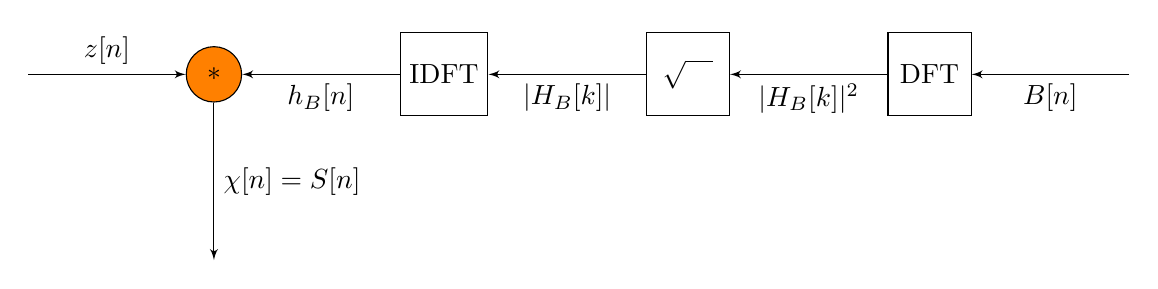
\begin{tikzpicture}[auto, node distance=2cm,>=latex']
\tikzset{
op/.style       = {draw, shape=circle, fill=orange, minimum height=2em, minimum width=2em},
block/.style    = {draw, shape=rectangle, fill=white, minimum height=3em, minimum width=3em},
coord/.style    = {coordinate},
}

    % Fluctuations nodes
    \node [op]                (fluct_conv)    {$\ast$};
    \node [coord, left=of fluct_conv]      (fluct_noise)   {};

    % Fluctuations edges
    \draw [->] (fluct_noise)-- node{$z[n]$}                 (fluct_conv);

    % Filter nodes
    \node [block, right=of fluct_conv]      (fluct_idft)    {IDFT};
    \node [block, right=of fluct_idft]      (fluct_spectrum){$\sqrt{\quad}$};
    \node [block, right=of fluct_spectrum]  (fluct_dft)     {DFT};
    \node [coord, right=of fluct_dft]       (fluct_ac)      {};
    % Filter edges
    \draw [->] (fluct_idft) --node{$h_B[n]$} (fluct_conv);
    \draw [->] (fluct_spectrum) -- node{$|H_B[k]|$} (fluct_idft);
    \draw [->] (fluct_dft) -- node{$|H_B[k]|^2$} (fluct_spectrum);
    \draw [->] (fluct_ac) -- node{$B[n]$} (fluct_dft);

    \node [coord, below=of fluct_conv]      (fluctuations)   {};
    \draw [->] (fluct_conv)-- node{$\chi[n]=S[n]$}                 (fluctuations);

\end{tikzpicture}
  \caption{Block diagram of signal processing steps for generating scintillations. Gaussian white noise $z[n]$ is convolved with an impulse response $h_B[n]$ which is based on the covariance $B[n]$ of the turbulence spectrum.}
  \label{fig:generating_block_diagram_simple}
\end{figure}

\subsection{Apply scintillations to signal}
Now that we can generate sequences of fluctuations, we need to apply these to a
carrier signal $x(t)$ or $x[n]$. According to equation
\eqref{eq:generating_sequences_multiplicative} the log-amplitude fluctuations can
be applied in a multiplicative manner, which is indeed the case of a signal with
a sufficiently small bandwidth, like for example a monochromatic signal.
However, the variance of the fluctuations is frequency-dependent, and since in
practice broadband signals are commonly used, a method is sought for applying the
fluctuations to a broadband signal.

One possible method would be to decompose the input signal in complex
exponentials with the Inverse Discrete Fourier Transform, and apply per complex
exponential the log-amplitude and phase fluctuations which, when combined, can be
written as a complex exponential as shown in equations
\eqref{eq:complex_exponential} and \eqref{eq:chi_and_S}.

A computationally less demanding method is to instead filter the carrier signal
with multiple band-pass filters, and proceed with applying fluctuations to each
of the band-pass filtered signals and combining the resulting signals.
Scintillations would be computed for the center frequencies of the bands. The amplitude
fluctuations could be applied through multiplication and the phase
fluctuations could be converted to time-delay fluctuations (see equation
\eqref{eq:time_delay_fluctuations}) and applied with a Variable Delay Line (VDL).


\subsection{Scintillations as time-variant filter}
A more efficient method to take into account the frequency-dependence
of the scintillations, would be to instead convolve the carrier signal with a
time-variant filter that is updated fast enough to represent the fluctuations.

The fluctuations $\chi$ and $S$, at each time step computed for $M_2$ frequencies, can be merged into a complex phase (see equation \eqref{eq:chi_and_S})
\begin{equation}
 \psi[n] = \exp\left({\chi[n] + jS[n] }\right)
\end{equation}
Adding a linear-phase factor as was done with $h_B[n]$ and taking the Inverse
Discrete Fourier Transform will result in an impulse response for every instance
in time $n$. Convolution of the carrier signal $x[n]$ with this time-variant
filter will result in a log-amplitude and phase modulated signal. The first
$M_2/2$ samples will have to be dropped to correct for the filter delay.

Because the fluctuations are relatively low-frequent they can be sampled at a
much lower sample frequency than the carrier signal. For a correlation length
$L$ of 10 meters and a transverse speed $v_{\bot}$ of 2 meters per second the
correlation time would be 5 seconds. If we would sample the sequence of
fluctuations at 5 times the maximum bandwidth of the filter, which is
proportional to the inverse of the correlation time $\tau_0$,
\begin{equation}
 f_s = 5 / \tau_0
\end{equation}
the required sample frequency would be 1 hertz.

In practice one might want to interpolate the impulse response as it changes
over time, but because the phase also changes with time this can be problematic.
Aside from converting to a minimum-phase representation we can also create a
linear-phase filter for which the magnitude changes with time but the phase does
not. If the phase fluctuations are linear-phase, then they can be applied to the
carrier signal $x[n]$ with a Variable Delay Line. In the Gaussian model the
phase fluctuations scale as $\sigma_S^2 \sim f^2$. A scatterer affects all frequencies, and therefore the fluctuations of different frequencies move together, resulting in a linear-phase.
We therefore write the phase fluctuation $\mathrm{d}S(t)$ as a propagation delay fluctuation
\begin{equation}\label{eq:time_delay_fluctuations}
\mathrm{d}t(t) = \mathrm{d}S(t) / (2 \pi f)
\end{equation}
% \todo{How does this fit with the channel, eqs. 19-22}
or in discrete time
\begin{equation}
 \mathrm{d}[n] = \mathrm{d}S[n] / (2 \pi k f_s)
\end{equation}

With the Gaussian turbulence spectrum it is straightforward to separate the
covariance $B(\tau)$ into the correlation $C(\tau)$ and variance $\sigma$ as defined in respectively equations \eqref{eq:gaussian_correlation} and \eqref{eq:model_daigle}. That
way we can compute a filter $h_C[n]$ that depends solely on the correlation
$C(\tau)$, and scale this afterwards with the correct variances $\sigma_{\chi}$
and $\sigma_{S}$. The advantage is having to compute only one sequence of
fluctuations, which is determined entirely by the covariance and $z[n]$, and can
then be scaled with the (frequency-dependent) variances $\sigma_{\chi}$ and
$S$.

\subsection{Moving source}
Thus far it was assumed neither the source nor the receiver were moving, and
that the fluctuations arise due to sampling a turbulent field that is moving
by with constant speed at a fixed receiver position.

If the field is transported faster, the spatial fluctuations are sampled faster,
and therefore the scintillations $\chi[n]=S[n]$ are compressed in time
corresponding to fluctuations with relatively higher frequencies.

In case the turbulent field is transported by wind and neither source nor
receiver are moving, the source-receiver distance remains constant. If we
instead consider a moving source of which the emitted sound samples the turbulent field, then the
source-receiver distance $d$ generally changes and thus also the variances $\sigma_{\chi}$ and $\sigma_{S}$.

We will now consider a moving source. The transverse velocity is in this case
the velocity component of the moving source, perpendicular to the wave
propagation direction. This is the vector \emph{rejection} of the source
velocity vector $\mathbf{v_s}$ from the unit vector $\mathbf{\hat{o}}$ that
represents the orientation from source to receiver. The transverse speed is the
norm of this vector
\begin{equation}
 v_{\bot} = \left\| \mathbf{v_s} - (\mathbf{v_s} \cdot  \mathbf{\hat{o}} ) \cdot \mathbf{\hat{o}}  \right\|
%  v_{\bot} = \left\| \mathbf{\hat{o}} \times \mathbf{v_s} \right\|
\end{equation}
The vector \emph{projection} of the source velocity on the wave propagation
direction is the component that is relevant for the Doppler shift. Therefore, as
the Doppler shift is maximum the modulations are relatively low-frequent,
whereas if the Doppler shift is zero, the modulations are relatively
high-frequent.

When computing two sequences of scintillations, but for different
transverse speeds, one does not obtain a compressed version of the other using
the method as described thus far in this section, even when using the same seed
for the Pseudo-Random Number Generator. This is because, by adjusting $v_{\bot}$,
we effectively applied the compression on the filter $h_C[n]$ before convolution
with $z[n]$. Therefore, the two resulting sequences will not look compressed in
time, but instead just filtered differently. Even so, the generated sequence will
have the desired statistical properties.

We can obtain the desired compression, i.e., scaling in time, if we instead
perform the convolution between $z[n]$ and a time-invariant $h_C[n]$ computed for a fixed $\tau_0$, $\tau_{\mathrm{ref}}$, and then
resample the values of $\chi[n]$ and $S[n]$ at different times to take into
account the change in correlation. Instead of having a constant sample timestep
\begin{equation}
 t_k = \frac{k}{f_s} = \sum_{i=0}^k \frac{1}{f_s}, \quad k=0, 1, \dots, \quad i=0, 1, \dots
\end{equation}
the sample time varies with correlation time
\begin{equation}
  t_k = \sum_{i=0}^k \frac{\tau_{\mathrm{ref}}}{\tau_{0,i}} \frac{1}{f_s} , \quad k=0, 1, \dots, \quad i=0, 1, \dots
\end{equation}

Figure \ref{fig:generating_block_diagram} shows the full block diagram of the signal
processing steps for generating scintillations and including them in an auralization.


\subsection{Saturation of the log-amplitude fluctuations}
According to equation \eqref{eq:model_daigle} the fluctuations increase with distance and frequency indefinitely.
For longer path lengths or stronger turbulence, the amplitude fluctuations
gradually level off. Saturation of the amplitude fluctuations can be observed
when measuring aircraft noise at distances of over a few kilometers. The
standard deviation of the fluctuating sound pressure levels is in such cases
limited to approximately 6 dB \cite{Daigle1983}.

Saturation of the log-amplitude fluctuations can be included based on an analysis by Wenzel
\cite{Wenzel1975}. In Wenzel's approach the soundwave is split up in a coherent
and incoherent wave. The amplitude of the coherent wave decreases over distance
while the incoherent wave obtains the energy from the coherent wave. The
coherent wave $p$ is written as
\begin{equation}
 \langle p \  p^* \rangle = \left( A_m^2 / 4 \pi r^2 \right) \exp{\left( -2 \langle \mu^2 \rangle k^2 r L \right)}
\end{equation}
Wenzel defines the distance to saturation $r_s$ as the distance at which the coherent wave is reduced to $e^{-1}$ of its original strength
\begin{equation}\label{eq:saturation_distance}
 r_s = \frac{1}{2 \sigma_{\mu}^2 k^2 L}
\end{equation}
Saturation of the log-amplitude fluctuations can now be included by multiplying the log-amplitude with a correction factor.
The variance of log-amplitude fluctuations that includes saturation $\sigma_{\chi}$, is given by
\begin{equation}\label{eq:saturation_logamp}
 \sigma_{\chi, sat} = \sigma_{\chi} \frac{ 1}{1 + r/r_s}
\end{equation}

\begin{figure}[H]
  \centering
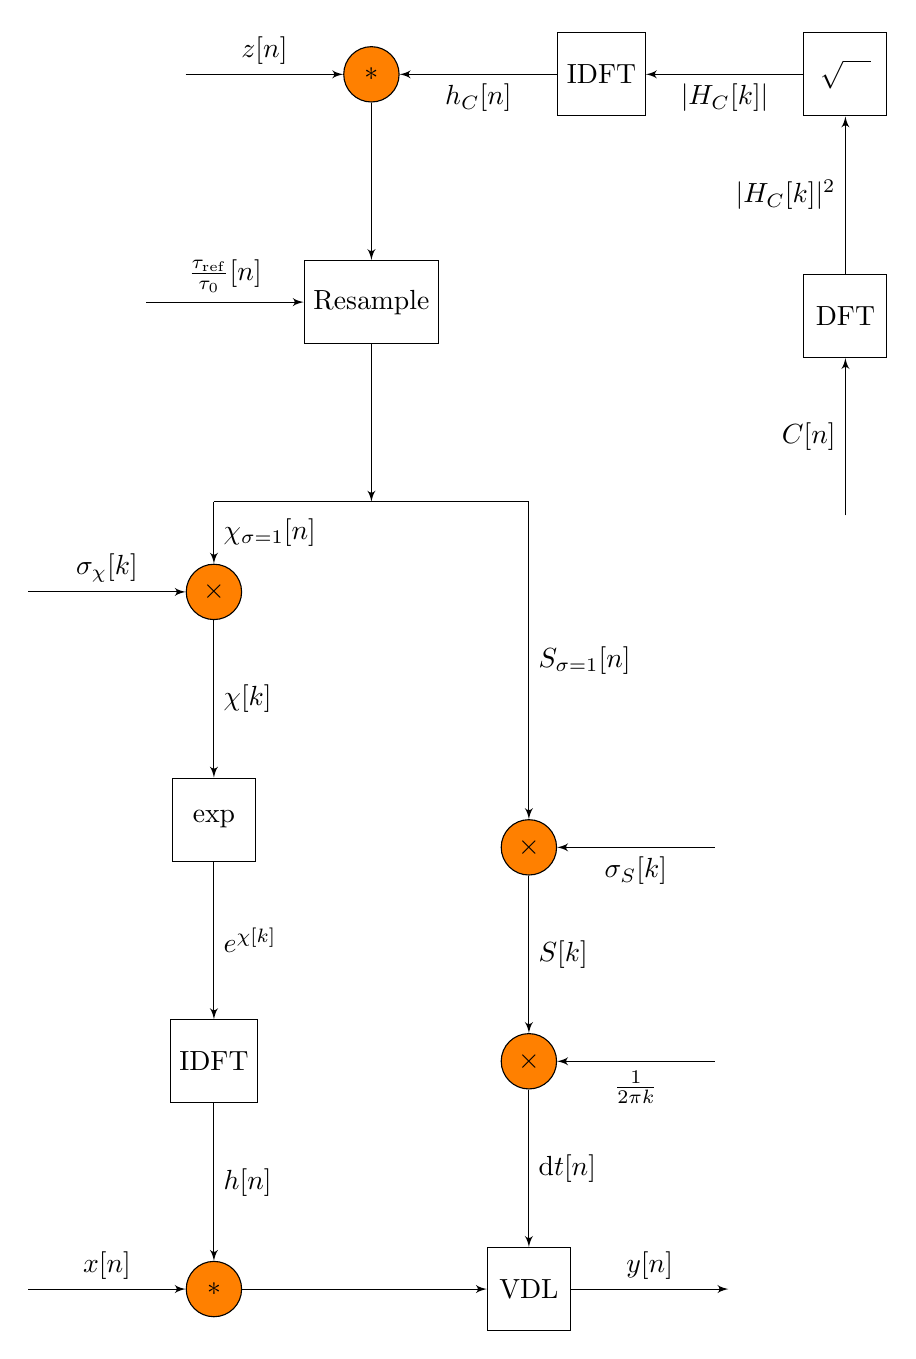
\begin{tikzpicture}[auto, node distance=2cm,>=latex']
\tikzset{
op/.style       = {draw, shape=circle, fill=orange, minimum height=2em, minimum width=2em},
block/.style    = {draw, shape=rectangle, fill=white, minimum height=3em, minimum width=3em},
coord/.style    = {coordinate},
}
    % Apply nodes
    \node [op]              (apply_conv) at (-2, 0)   {$\ast$};
    \node [coord, left=of apply_conv]                           (input)         {};
    \node [block]      (apply_vdl) at (+2, 0)    {VDL};
    \node [coord, right=of apply_vdl]       (output)        {};

    % Apply edges
    \draw [->] (input)      -- node{$x[n]$}                 (apply_conv);
    \draw [->] (apply_conv) --                              (apply_vdl);
    \draw [->] (apply_vdl)  -- node{$y[n]$}                 (output);

    % Amplitude nodes
    \node [block, above=of apply_conv]      (apply_ir)      {IDFT};
    \node [block, above=of apply_ir]        (a_exp)         {exp};
    \node [op, above=of a_exp]              (a_apply_var)   {$\times$};
    \node [coord, left=of a_apply_var]      (a_var)         {};
    \node [coord]     (a_tee) at (-2, 10)      {};

    % Amplitude edges
    \draw [->] (a_tee)      -- node{$\chi_{\sigma=1}[n]$}            (a_apply_var);
    \draw [->] (a_var)      -- node{$\sigma_{\chi}[k]$}  (a_apply_var);
    \draw [->] (a_apply_var)-- node{$\chi[k]$}            (a_exp);
    \draw [->] (a_exp)      -- node{$e^{\chi[k]}$}        (apply_ir);
    \draw [->] (apply_ir)   -- node{$h[n]$}               (apply_conv);

    % Phase nodes
    \node [op, above=of apply_vdl]          (p_to_delay)    {$\times$};
    \node [op, above=of p_to_delay]         (p_apply_var)   {$\times$};
    \node [coord, right=of p_apply_var]     (p_var)         {};
    \node [coord, right=of p_to_delay]      (p_delay)       {};
    \node [coord]     (p_tee)  at (+2, 10)       {};

    % Phase edges
    \draw [->] (p_to_delay) -- node{$\mathrm{d}t[n]$}       (apply_vdl);
    \draw [->] (p_apply_var)-- node{$S[k]$}              (p_to_delay);
    \draw [->] (p_var)      -- node{$\sigma_S[k]$}        (p_apply_var);
    \draw [->] (p_delay)    -- node{$\frac{1}{2 \pi k}$}    (p_to_delay);
    \draw [->] (p_tee)      -- node{$S_{\sigma=1}[n]$}               (p_apply_var);

    % Fluctuations nodes
    \node [coord] (tee) at (0, 10) {};
    \node [block, above=of tee]                (fluct_resample)     {Resample};
%     \node [coord, right=of a_tee]           (tee)           {};
    \node [op, above=of fluct_resample]                (fluct_conv)    {$\ast$};
    \node [coord, left=of fluct_conv]      (fluct_noise)   {};
    \node [coord, left=of fluct_resample] (correlation_time_rel) {};

    \draw [->] (correlation_time_rel) -- node{$\frac{\tau_{\mathrm{ref}}}{\tau_{0}}[n]$}  (fluct_resample);

    % Fluctuations edges
    \draw [->] (fluct_noise)-- node{$z[n]$}                 (fluct_conv);
    \draw [->] (fluct_conv) --                              (fluct_resample);
    \draw [->] (fluct_resample)  --                              (tee);
    \draw [-]  (tee)        --                              (a_tee);
    \draw [-]  (tee)        --                               (p_tee);

    % Filter nodes
    \node [block, right=of fluct_conv]      (fluct_idft)    {IDFT};
    \node [block, right=of fluct_idft]      (fluct_spectrum){$\sqrt{\quad}$};
    \node [block, below=of fluct_spectrum]  (fluct_dft)     {DFT};
    \node [coord, below=of fluct_dft]       (fluct_ac)      {};
    % Filter edges
    \draw [->] (fluct_idft) --node{$h_{C}[n]$} (fluct_conv);
    \draw [->] (fluct_spectrum) -- node{$|H_C[k]|$} (fluct_idft);
    \draw [->] (fluct_dft) -- node{$|H_C[k]|^2$} (fluct_spectrum);
    \draw [->] (fluct_ac) -- node{$C[n]$} (fluct_dft);


\end{tikzpicture}
  \caption{Block diagram of signal processing steps.}
  \label{fig:generating_block_diagram}
\end{figure}

\section{Results}

\subsection{A single tone}
To demonstrate the model we shall now consider a tone of 1000 Hz and apply modulations to the tone.
The following parameters are used: $c=343.2$
m/s, $\sigma_{\mu}^2=3\cdot10^{-6}$, $L=1.1$ m, $v_{\bot}=2.0$ m/s and $d=500$
m. Saturation according to equation \eqref{eq:saturation_logamp} is also included.
The filter $h_c$ is designed to have 8192 taps. The correlation time is then
$\tau=L/v_{\bot}=0.55$ s and the sample frequency at which the modulations are
generated $5/\tau=9.1$ Hz.

Figure \ref{fig:results_tone_logamp_and_phase} shows the time series of
amplitude and phase fluctuations that were generated. Figure
\ref{fig:results_tone_levels} shows the tone along with a modulated version of
the tone. The tone was sampled at 8000 Hz.

The log-amplitude and phase move in-phase. The value for the log-amplitude is slightly lower than that of the phase because of saturation.
As expected the phase fluctuations cause spectral broadening of the tone as can be seen in Figure \cite{Ostashev2016}.

\begin{figure}[H]
  \centering
  \includegraphics[]{../figures/generated/turbulence-tone/logamp_and_phase}
  \caption{Amplitude and phase fluctuations as function of time. The fluctuations are less strong for the amplitude fluctuations due to saturation.}
  \label{fig:results_tone_logamp_and_phase}
\end{figure}

\begin{figure}[H]
  \centering
  \includegraphics[]{../figures/generated/turbulence-tone/modulated_levels}
  \caption{Sound pressure level of the tone as function of time, with and without fluctuations.}
  \label{fig:results_tone_levels}
\end{figure}



\begin{figure}[H]
  \centering
  \includegraphics[]{../figures/generated/turbulence-tone/tone_broadening}
  \caption{The power spectrum of the tone shows the broadening due to the phase fluctuations.}
  \label{fig:results_tone_broadening}
\end{figure}

\subsection{Scintillations as function of transverse speed}
By changing the transverse speed the refractive-index field is sampled at a
different speed. This effectively changes the correlation length and shifts the frequency range that is covered by our applied filter \cite{Wilson1999}.

Figure \ref{fig:results_scintillations_correlation} shows the correlation function for
different transverse speeds.
\begin{figure}[H]
  \centering
  \includegraphics[]{../figures/generated/turbulence-tone/correlation}
  \caption{Correlation as function of time for different transverse speeds given in meters per second.}
  \label{fig:results_scintillations_correlation}
\end{figure}
With a high transverse speed the correlation drops
faster, and this will result in relatively more high-frequency fluctuations, as is shown in Figure \ref{fig:results_scintillations_levels}.
\begin{figure}[H]
  \centering
  \includegraphics[]{../figures/generated/turbulence-tone/scintillations_levels}
  \caption{Sound pressure level as function of time for scintillations
corresponding to different transverse speeds given in meters per second. The
same $z[n]$ were used for each case. A compression in time of the modulations with increasing velocity can be observed.}
  \label{fig:results_scintillations_levels}
\end{figure}


\subsection{Application in auralization of aircraft}
The method was developed in order to create more realistic sounding
auralizations of aircraft. An aircraft moves at high speed through the
atmosphere. A transverse speed is computed for each propagation path separately.
Because the correlation time, distance and propagation varies between the two
paths, decorrelation occurs. Figures \ref{fig:results_auralization_without} and
\ref{fig:results_auralization_with} show spectrograms respectively with and
without turbulence. The vertical lines that can be seen are the amplitude
modulations.

\begin{figure}[H]
  \centering
  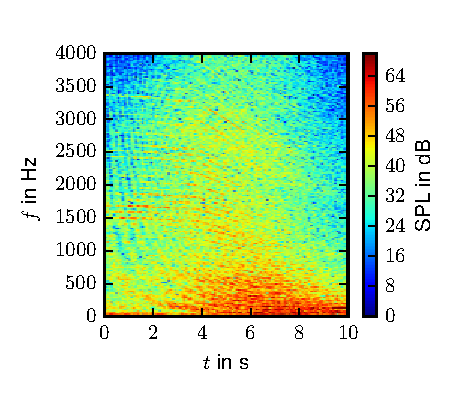
\includegraphics[]{../figures/manual/turbulence-model/auralisation_flight_without}
  \caption{Spectrogram of an auralization of an aircraft taking off.
Scintillations were not included. Visible are the ground effect and the Doppler
shift. In the initial seconds a high amount of tonal components are visible.
  }
  \label{fig:results_auralization_without}
\end{figure}

\begin{figure}[H]
  \centering
  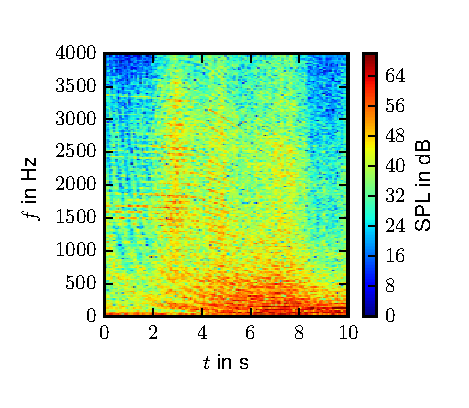
\includegraphics[]{../figures/manual/turbulence-model/auralisation_flight_both}
  \caption{Spectrogram of the same event as in Figure
  \ref{fig:results_auralization_without}, however, this time with scintillations included. Because of the high speed at which the aircraft samples the refractive-index field the scintillations are relatively high-frequent, resulting in vertical lines.}
  \label{fig:results_auralization_with}
\end{figure}

Earlier it was assumed that the correlation length was much smaller than the Fresnel zone size.
In this auralization the aircraft is moving close to the receiver. When the aircraft is closest, the distance is almost entirely given by the height which was approximately 100 meters.
The correlation length was set at 20 meters. In that case the Fresnel zone is larger than the correlation length for the lower frequencies, and equation \eqref{eq:model_daigle} is not valid.
Instead, the log-amplitude and phase variances should scale with respectively $d^3$ and $2k^2 d$ instead of $k^2 d$ \cite{Ishimaru1997}.


\subsection{Influence of parameters}

\begin{figure}[H]
%     \centering
    \begin{subfigure}{\textwidth}
        \includegraphics{{{../figures/generated/turbulence-parameters/turbulence-1.0-1e-05}}}
        \caption{\SI{1}{\meter}}
    \end{subfigure}
    ~
    \begin{subfigure}{\textwidth}
        \includegraphics{{{../figures/generated/turbulence-parameters/turbulence-10.0-1e-05}}}
        \caption{\SI{10}{\meter}}
    \end{subfigure}
    ~
    \begin{subfigure}{\textwidth}
        \includegraphics[]{{{../figures/generated/turbulence-parameters/turbulence-100.0-1e-05}}}
        \caption{\SI{100}{\meter}}
    \end{subfigure}
    \caption{The influence of the correlation length $L$. The variance of the dynamic refractive-index is $\SI{1e-5}{}$.}
    \label{fig:turbulence:aircraft:parameters:correlation}
\end{figure}

\newpage
\begin{figure}[H]
%     \centering
    \begin{subfigure}{\textwidth}
        \includegraphics{{{../figures/generated/turbulence-parameters/turbulence-10.0-1e-05}}}
        \caption{\SI{1e-5}{}}
    \end{subfigure}
    ~
    \begin{subfigure}{\textwidth}
        \includegraphics{{{../figures/generated/turbulence-parameters/turbulence-10.0-1e-06}}}
        \caption{\SI{1e-6}{}}
    \end{subfigure}
    ~
    \begin{subfigure}{\textwidth}
        \includegraphics[]{{{../figures/generated/turbulence-parameters/turbulence-10.0-1e-07}}}
        \caption{\SI{1e-7}{}}
    \end{subfigure}
    \caption{The influence of the variance of the dynamic refractive-index $\sigma_{\mu}^2$. The correlation length is \SI{1}{\meter}.}
    \label{fig:turbulence:aircraft:parameters:variance}
\end{figure}


\section{Conclusion}
Fluctuations in the refractive-index field due to variations in temperature and
wind affects sound propagation and causes audible modulations. A method was
presented for generating sequences of modulations and applying these to
monochromatic as well as broadband signals.

A Rytov approximation to first-order refractive-index flucutuations results in a complex
phase which we can write as a log-amplitude $\chi$ and phase $S$ fluctuation.
The propagating sound is modelled as a time-varying channel where we consider
two sequences, one for the log-amplitude fluctuations, and another for the phase
fluctuations.

The fluctuations are frequency-dependent and therefore a filter was designed to take that into account.
% A Gaussian applied filter was used to model the atmospheric turbulence because of its simplicity and because it is computationally least demanding.
A Gaussian turbulence spectrum was considered, but the general method can be
used with other turbulence spectra as well. The Von Karman spectrum describes
real turbulence spectra typically better than the Gaussian spectrum, however,
the Von Karman spectrum is computationally much more demanding.
% The Gaussian model also allows implementing the phase fluctuation with a Variable Delay Line (VDL).

Examples are shown where the method is applied to a tone and to an aircraft
auralization. The aircraft auralization spectrogram shows several spikes
corresponding to amplitude modulations as well as an increase in the amount of
decorrelation. Furthermore the transverse velocity dependence on the frequency
content of the modulations is demonstrated.

According to the author the method results in more realistic sounding
auralizations, but this has not been validated yet with listening tests. The
implementation of the model that was used in this paper to generate the figures
can be found at \cite{Rietdijk2016}.


% \input{implementation_turbulence}

% \input{implementation_reproduction}

\chapter{Subjective validation of synthesis method}\label{chapter:test}\todo{From paper. Rewrite}

\section{Introduction}


\section{Method}

A listening test was conducted to determine whether the auralisations sound
similar to the recordings they were based on. Participants were presented with
pairs of stimuli and asked to rate how similar they sounded.

% \todo{explain why this method is chosen? Explain other available methods?}
% One can think of multiple methods to
% determine the similarity. The MUSHRA (MUltiple Stimuli with Hidden Reference and
% Anchor) test is methodology used for evaluating audio quality \cite{}, and has also been used for determining the plausibility of synthesised vehicle pass-by sounds when compared to recordings \cite{Southern2016}.

Eight different stimuli were considered and they were 12 seconds long.
Because the sounds vary considerably over time, they were each split into parts
of 4 seconds, corresponding to the approach, fly-over and distancing. For each
part all combinations were considered. Each part therefore consisted of 28 pairs
of stimuli of four seconds.

Of the eight stimuli four were recordings, and four were auralisations with each
of them based on one of the recordings. Two aircraft types were considered, an
A320 and a RJ1H, and two events per aircraft type.
% The recordings were made close to the airport. \todo{this sentence can be dropped if we have a Measurements section}
% with the aircraft passing by at approximately 90 meters.
Headphones were used and HRTF's were not included.

Because similarity is relative, an anchor is typically used. In this test the
participants were for each part first given the set of stimuli, in order to
become familiar with the type of sounds and the spread in the sounds of that
part, and then continued with rating the pairs. The rating was done on an eleven
point Likert scale. The left side of the scale said ``not so much'' and the right
side ``very much''. The scale was not numbered.


\section{Results}
The results of the participants were scaled linearly from 0 to 1 with 0
correspond to ``not so much'' and 1 corresponding to ``very much''. Since not
all participants used the full scale, they were rescaled per participant to use
the full scale. There were 17 participants, all graduate students, and of which
the majority studied acoustics. The results that are shown are obtained after
joining the data of all participants and all three test parts.

Figure \ref{fig:ratings_recordings} shows the similarity ratings grouped per
aircraft combination, considering only recordings. Figure
\ref{fig:ratings_simulations} shows the similarity ratings grouped per
aircraft combination, but now for the auralisations.
Figures \ref{fig:ratings_A320} and \ref{fig:ratings_RJ1H} show
for respectively the A320 and the RJ1H the similarity ratings grouped per pairs
of stimuli type, that is, recordings and/or simulations.
The listening test and results can be found at respectively \cite{Rietdijk2017a} and \cite{Rietdijk2017b}.

% \begin{figure}[H]
%   \centering
%   \includegraphics[]{figure_ratings}
%   \caption{Similarity ratings for different groups.}
%   \label{fig:ratings
% \end{figure}

\begin{figure}[H]
  \centering
  \includegraphics[]{../figures/manual/auralisation-paper/figure1_ratings_recordings}
  \caption{Similarity ratings for the recordings grouped by aircraft type.}
  \label{fig:ratings_recordings}
\end{figure}

\begin{figure}[H]
  \centering
  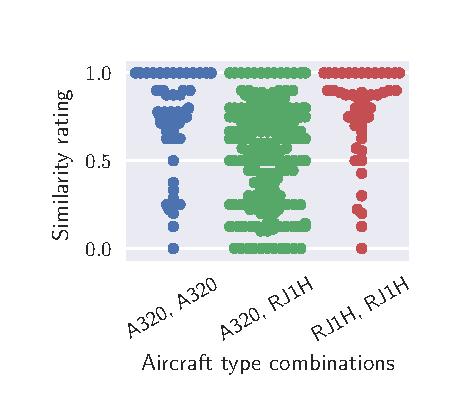
\includegraphics[]{../figures/manual/auralisation-paper/figure2_ratings_simulations}
  \caption{Similarity ratings for the auralisations grouped by aircraft type.}
  \label{fig:ratings_simulations}
\end{figure}

\begin{figure}[H]
  \centering
  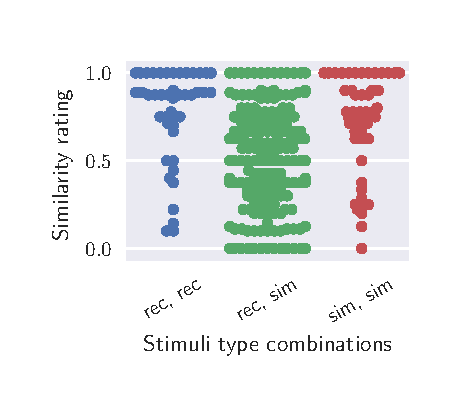
\includegraphics[]{../figures/manual/auralisation-paper/figure3_ratings_A320}
  \caption{Similarity ratings for the A320 grouped by stimuli type combinations.}
  \label{fig:ratings_A320}
\end{figure}

\begin{figure}[H]
  \centering
  \includegraphics[]{../figures/manual/auralisation-paper/figure4_ratings_RJ1H}
  \caption{Similarity ratings for the RJ1H grouped by stimuli type combinations.}
  \label{fig:ratings_RJ1H}
\end{figure}

The ratings were obtained for three different parts of the stimuli, ``start'',
``center'' and ``end'', and that allows us to also group the ratings by each of
these parts. Figures \ref{fig:ratings_part_A320} and \ref{fig:ratings_part_RJ1H}
show the similarity ratings for respectively the A320 and RJ1H grouped per
stimuli type combination and per stimuli part. A Tukey boxplot is used to
improve the clarity of the figure.

\begin{figure}[H]
  \centering
  \includegraphics[]{../figures/manual/auralisation-paper/figure5_ratings_part_A320}
  \caption{Similarity ratings for the A320 grouped by stimuli type combinations and stimuli part.}
  \label{fig:ratings_part_A320}
\end{figure}

\begin{figure}[H]
  \centering
  \includegraphics[]{../figures/manual/auralisation-paper/figure6_ratings_part_RJ1H}
  \caption{Similarity ratings for the RJ1H grouped by stimuli type combinations and stimuli part.}
  \label{fig:ratings_part_RJ1H}
\end{figure}

Participants mentioned they noted larger differences at especially the beginning
of the events (``start`` parts) and also at the end of the events (``end`` parts). A
common answer to the question how many aircraft they heard was ``two or three``.
Occasionally, the answer would start at ``two`` but go to ``two or more`` after they
were told they were listening to not only recordings but also simulations. Some
participants were surprised when told that simulations were included,
others said they had thought so, and a few of the participants were already
aware the test was possibly going to contain simulations.

\section{Discussion}
As can be seen in Figure \ref{fig:ratings_recordings}, the A320's are judged to be very
similar to each other, and the RJ1H's as quite similar to each other. The A320's
are not rated as very similar to the RJ1H's and therefore we conclude that the
participants can discriminate between the two aircraft types.

In the case of the auralisations, Figure \ref{fig:ratings_simulations}, the
participants can also discriminate between the aircraft types, but now the
RJ1H's are judged to be relatively more similar than the A320's. Compared to the recordings
the difference between the A320's and the RJ1H's is slightly smaller.

% One might argue from these findings that the whole set of auralisations is more similar than the set of recordings.

Figures \ref{fig:ratings_A320} and \ref{fig:ratings_RJ1H} show
as additional information how similar the auralisations are to the recordings.
The groups ``(rec, sim)'' contain pairs consisting of a recording and an
auralisation. The similarity ratings for these two groups are similar to the
``(A320, RJ1H)'' groups in Figures \ref{fig:ratings_recordings} and
\ref{fig:ratings_simulations}. Therefore, it would appear that listeners can
discriminate between aircraft types, but that the auralisations are considered
to be of different aircraft types than the recordings they're based on.

Figures \ref{fig:ratings_part_A320} and \ref{fig:ratings_part_RJ1H} show the
same data but now further grouped by stimuli part. Judging from Figure
\ref{fig:ratings_part_A320} there appears to be a relative large dissimilarity
between the ``start'' parts of the A320 recordings and also between the ``end''
parts of the A320 auralisations. The groups ``(rec, rec)'' and ``(sim, sim)''
consist however of only 17 data points each whereas the ``(rec, sim)'' group
has 68 data points.

The participants mentioned relatively larger differences in the stimuli that
correspond to the approach of the aircraft (``start`` stimuli). During the
approach the tonal components are clearly audible compared to other parts of the
events due to the directivity. The feature-extraction algorithm was known to
underestimate the power and bandwidth of the blade passing frequency and its
harmonics because the algorithm was tuned for the Buzz-Saw tones. Therefore, a
likely explanation is that this underestimation of power and bandwidth is
causing audible differences between recordings and auralisations.




\chapter{Conclusions and future work}\label{chapter:conclusions}

\section{Conclusions}

% TODO: comment Jens, sounds plausible

% Overview paper
Aircraft noise has a negative impact on humans. To further study its impact on
humans a tool was developed to simulate the audible sound field caused by
fly-overs of airplanes. The goal was to develop a tool that can create
auralisations of the current fleet of aircraft.

The auralisation tool consists of an emission synthesiser and a propagation
model based on geometrical acoustics. Emission synthesiser used spectral
modelling synthesis as synthesis strategy and used features extracted from
recordings as input. These features were automatically extracted from a signal
that was obtained after applying an inverse propagation model to a recording.
To verify whether the auralisations sound similar to recordings of the
respective airplane types, a listening test was conducted.

Participants were presented with a paired comparison test. Participants were
able to discriminate between sounds of different aircraft types, in case of both
recordings and auralisations. The similarity ratings between recordings and
auralisations are roughly similar to the similarity ratings between the two
aircraft type. That would imply the auralisations sound like different aircraft
than those that were recorded.

An incorrect reproduction of the blade passing frequency and its harmonics is
the likely cause of the dissimilatity between the auralisations and recordings.
The feature-extraction algorithm was tuned for the relatively small bandwidth of
the Buzz-Saw tones and is therefore underestimating the power and bandwidth of
the blade-passing frequency and harmonics.

Section \ref{sec:introduction:background:auralisation} listed several
auralisation use cases. Whether it is relevant that the auralisations do not
sound exactly similar to the recordings would depend on how the auralisations
would be utilised.

% Turbulence paper
To improve the plausibility of the auralisations
% in situations where the source-receiver distance is typically larger
a method was developed to simulate modulations due to atmospheric turbulence.
Spatial and temporal variations in temperature and cause variations in the soundspeed field.
As sound propagates through a turbulent atmosphere, the variations will cause
multiple scattering and result in audible modulations, known as scintillations.
A method was presented for generating sequences of modulations and applying
these to both monochromatic and broadband signals.

% TODO rewrite rest of section (turbulence paper)

A Rytov approximation to first-order refractive-index fluctuations results in a complex
phase which we can write as a log-amplitude $\chi$ and phase $S$ fluctuation.
The propagating sound is modelled as a time-varying channel where we consider
two sequences, one for the log-amplitude fluctuations, and another for the phase
fluctuations.

The fluctuations are frequency-dependent and therefore a filter was designed to take that into account.
% A Gaussian applied filter was used to model the atmospheric turbulence because of its simplicity and because it is computationally least demanding.
A Gaussian turbulence spectrum was considered, but the general method can be
used with other turbulence spectra as well. The Von Karman spectrum describes
real turbulence spectra typically better than the Gaussian spectrum, however,
the Von Karman spectrum is computationally much more demanding.
% The Gaussian model also allows implementing the phase fluctuation with a Variable Delay Line (VDL).

Examples are shown where the method is applied to a tone and to an aircraft
auralization. The aircraft auralization spectrogram shows several spikes
corresponding to amplitude modulations as well as an increase in the amount of
decorrelation. Furthermore the transverse velocity dependence on the frequency
content of the modulations is demonstrated.

The method seems to result in more realistic sounding
auralizations, but this has not been validated yet with listening tests. The
implementation of the model that was used in this paper to generate the figures
can be found at \cite{Rietdijk2016}.

\section{Future work}
Future steps to be taken depends strongly on how auralisations would
be used.
% The next steps to be taken depend on how auralisations would be used.

\subsubsection*{Investigate human response to aircraft sound}
If one wants to study humans' response to aircraft sound, then the next step is
to test whether auralisations of aircraft are sufficiently similar to the actual
sound of aircraft, with respect to the parameter that is being investigated. If
the conclusion is that auralisations and recordings give sufficiently similar
results, then that would imply the auralisation method can be used to further
study that aspect of human response within the domain that was considered. If
significant differences would still be found, it would have to be tested what is
causing the differences.

% TODO comment Jens
% Future work: I suggest to add some example for the reader, at "If one wants to study humans’ response to aircraft sound, then the next step is to test whether auralisations of aircraft are sufficiently similar to the actual sound of aircraft, with respect to the parameter that is being investigated", like e.g. ", e.g. perceived annoyance or sleep disturbance."

\subsubsection*{Improve estimation and synthesis of blade passing frequency}
From the study that was conducted and presented in this work, it followed that
participants did indeed notice differences between the auralisations and the
recordings. A probable cause of these differences is the estimation of the
power and bandwidth of the blade passing frequency and harmonics. Therefore, a
possible improvement would be to enhance the feature-extraction algorithm to
better estimate these properties.

% The most important point to improve is likely the simulation of the
% blade passing frequency and harmonics, and that would require a better
% estimation of their powers and bandwidths. Aside from that, it would seem the
% auralisation tool is capable of delivering plausible auralisations.

\subsubsection*{Develop generic aircraft emission model}
Because the auralisations appear to sound plausible it is concluded that the strategy\todo{what strategy? recording, backprop, ...}
utilised works and therefore


\subsection{Scintillations}

\subsubsection*{Validate scintillations model}
The scintillations model is based on an existing statistical model.

\subsubsection*{Different model for describing turbulence spectrum}
As mentioned in the text the basic method for generating scintillations should
also work with other models, like the Von Karman spectrum. The Gaussian model
was chosen for performance reasons, as its simplest, but also because it allowed
further optimisations. Future work could be to develop an optimised algorithm
that utilises other spectra like e.g. the Von Karman spectrum with the use of
expressions given in \cite{Ostashev2015}.

\subsubsection*{Non-isotropic and non-homogeneous atmosphere for the scintillations model}
% \subsubsection*{Height-dependent parameters for the scintillations model}
The current model assumes a isotropic and homogeneous atmosphere. In practice,
the atmosphere is neither and parameters like the correlation length $L$ and the
variance of the refractive-index fluctuations $\langle \mu^2 \rangle$ are
height-dependent \cite{Krasnenko2013}. Ostashev et al. gave formulas for plane
\cite{Ostashev1997b} and spherical \cite{Ostashev1997c} waves propagating
through an anisotropic atmosphere and studies numerically the variances and
correlation functions of the log-amplitude and phase fluctuations
\cite{Ostashev2004}.

\subsubsection*{Determine parameters for scintillations model}
The model that was presented for generating scintillations uses a Gaussian
correlation function. A Gaussian can be used as an applied filter to get a rough
approximation to the actual turbulence spectrum within a certain wavenumber
range. An open question is how to obtain adequate values for the correlation
length $L$ and the variance of the refractive-index fluctuations $\langle \mu^2
\rangle$. Values for both can be obtained with a setup as used by Daigle et. al.
\cite{Daigle1983}, however, with such a setup values can only be obtained at
relatively low heights.




% \subsection{Develop better indicators for annoyance and sleep disturbance}

% \chapter{Future work}

% \chapter{Conclusions and future work}\label{chapter:conclusions}

\section{Conclusions}

% TODO: comment Jens, sounds plausible

% Overview paper
Aircraft noise has a negative impact on humans. To further study its impact on
humans a tool was developed to simulate the audible sound field caused by
fly-overs of airplanes. The goal was to develop a tool that can create
auralisations of the current fleet of aircraft.

The auralisation tool consists of an emission synthesiser and a propagation
model based on geometrical acoustics. Emission synthesiser used spectral
modelling synthesis as synthesis strategy and used features extracted from
recordings as input. These features were automatically extracted from a signal
that was obtained after applying an inverse propagation model to a recording.
To verify whether the auralisations sound similar to recordings of the
respective airplane types, a listening test was conducted.

Participants were presented with a paired comparison test. Participants were
able to discriminate between sounds of different aircraft types, in case of both
recordings and auralisations. The similarity ratings between recordings and
auralisations are roughly similar to the similarity ratings between the two
aircraft type. That would imply the auralisations sound like different aircraft
than those that were recorded.

An incorrect reproduction of the blade passing frequency and its harmonics is
the likely cause of the dissimilatity between the auralisations and recordings.
The feature-extraction algorithm was tuned for the relatively small bandwidth of
the Buzz-Saw tones and is therefore underestimating the power and bandwidth of
the blade-passing frequency and harmonics.

Section \ref{sec:introduction:background:auralisation} listed several
auralisation use cases. Whether it is relevant that the auralisations do not
sound exactly similar to the recordings would depend on how the auralisations
would be utilised.

% Turbulence paper
To improve the plausibility of the auralisations
% in situations where the source-receiver distance is typically larger
a method was developed to simulate modulations due to atmospheric turbulence.
Spatial and temporal variations in temperature and cause variations in the soundspeed field.
As sound propagates through a turbulent atmosphere, the variations will cause
multiple scattering and result in audible modulations, known as scintillations.
A method was presented for generating sequences of modulations and applying
these to both monochromatic and broadband signals.

% TODO rewrite rest of section (turbulence paper)

A Rytov approximation to first-order refractive-index fluctuations results in a complex
phase which we can write as a log-amplitude $\chi$ and phase $S$ fluctuation.
The propagating sound is modelled as a time-varying channel where we consider
two sequences, one for the log-amplitude fluctuations, and another for the phase
fluctuations.

The fluctuations are frequency-dependent and therefore a filter was designed to take that into account.
% A Gaussian applied filter was used to model the atmospheric turbulence because of its simplicity and because it is computationally least demanding.
A Gaussian turbulence spectrum was considered, but the general method can be
used with other turbulence spectra as well. The Von Karman spectrum describes
real turbulence spectra typically better than the Gaussian spectrum, however,
the Von Karman spectrum is computationally much more demanding.
% The Gaussian model also allows implementing the phase fluctuation with a Variable Delay Line (VDL).

Examples are shown where the method is applied to a tone and to an aircraft
auralization. The aircraft auralization spectrogram shows several spikes
corresponding to amplitude modulations as well as an increase in the amount of
decorrelation. Furthermore the transverse velocity dependence on the frequency
content of the modulations is demonstrated.

The method seems to result in more realistic sounding
auralizations, but this has not been validated yet with listening tests. The
implementation of the model that was used in this paper to generate the figures
can be found at \cite{Rietdijk2016}.

\section{Future work}
Future steps to be taken depends strongly on how auralisations would
be used.
% The next steps to be taken depend on how auralisations would be used.

\subsubsection*{Investigate human response to aircraft sound}
If one wants to study humans' response to aircraft sound, then the next step is
to test whether auralisations of aircraft are sufficiently similar to the actual
sound of aircraft, with respect to the parameter that is being investigated. If
the conclusion is that auralisations and recordings give sufficiently similar
results, then that would imply the auralisation method can be used to further
study that aspect of human response within the domain that was considered. If
significant differences would still be found, it would have to be tested what is
causing the differences.

% TODO comment Jens
% Future work: I suggest to add some example for the reader, at "If one wants to study humans’ response to aircraft sound, then the next step is to test whether auralisations of aircraft are sufficiently similar to the actual sound of aircraft, with respect to the parameter that is being investigated", like e.g. ", e.g. perceived annoyance or sleep disturbance."

\subsubsection*{Improve estimation and synthesis of blade passing frequency}
From the study that was conducted and presented in this work, it followed that
participants did indeed notice differences between the auralisations and the
recordings. A probable cause of these differences is the estimation of the
power and bandwidth of the blade passing frequency and harmonics. Therefore, a
possible improvement would be to enhance the feature-extraction algorithm to
better estimate these properties.

% The most important point to improve is likely the simulation of the
% blade passing frequency and harmonics, and that would require a better
% estimation of their powers and bandwidths. Aside from that, it would seem the
% auralisation tool is capable of delivering plausible auralisations.

\subsubsection*{Develop generic aircraft emission model}
Because the auralisations appear to sound plausible it is concluded that the strategy\todo{what strategy? recording, backprop, ...}
utilised works and therefore


\subsection{Scintillations}

\subsubsection*{Validate scintillations model}
The scintillations model is based on an existing statistical model.

\subsubsection*{Different model for describing turbulence spectrum}
As mentioned in the text the basic method for generating scintillations should
also work with other models, like the Von Karman spectrum. The Gaussian model
was chosen for performance reasons, as its simplest, but also because it allowed
further optimisations. Future work could be to develop an optimised algorithm
that utilises other spectra like e.g. the Von Karman spectrum with the use of
expressions given in \cite{Ostashev2015}.

\subsubsection*{Non-isotropic and non-homogeneous atmosphere for the scintillations model}
% \subsubsection*{Height-dependent parameters for the scintillations model}
The current model assumes a isotropic and homogeneous atmosphere. In practice,
the atmosphere is neither and parameters like the correlation length $L$ and the
variance of the refractive-index fluctuations $\langle \mu^2 \rangle$ are
height-dependent \cite{Krasnenko2013}. Ostashev et al. gave formulas for plane
\cite{Ostashev1997b} and spherical \cite{Ostashev1997c} waves propagating
through an anisotropic atmosphere and studies numerically the variances and
correlation functions of the log-amplitude and phase fluctuations
\cite{Ostashev2004}.

\subsubsection*{Determine parameters for scintillations model}
The model that was presented for generating scintillations uses a Gaussian
correlation function. A Gaussian can be used as an applied filter to get a rough
approximation to the actual turbulence spectrum within a certain wavenumber
range. An open question is how to obtain adequate values for the correlation
length $L$ and the variance of the refractive-index fluctuations $\langle \mu^2
\rangle$. Values for both can be obtained with a setup as used by Daigle et. al.
\cite{Daigle1983}, however, with such a setup values can only be obtained at
relatively low heights.




% \subsection{Develop better indicators for annoyance and sleep disturbance}



\newpage
% \bibliographystyle{plain}
% \bibliography{references}
\printbibliography

\appendix
\newpage

% PAPERS

% \chapter{Paper A}
% \includepdf[pages=-]{../papers/scintillations}
% \chapter{Paper B}
% \includepdf[pages=-]{../papers/overview}


\end{document}
